%%%%%%%%%%%%%%%%%%%%%%%%%%%%%%%%%%%%%%%%%%%%%%%%%%%%%%%%%%%%%%%%%%%%%%%%%%%%%
%
% Package pgfplots.sty documentation. 
%
% Copyright 2007/2008 by Christian Feuersaenger.
%
% This program is free software: you can redistribute it and/or modify
% it under the terms of the GNU General Public License as published by
% the Free Software Foundation, either version 3 of the License, or
% (at your option) any later version.
% 
% This program is distributed in the hope that it will be useful,
% but WITHOUT ANY WARRANTY; without even the implied warranty of
% MERCHANTABILITY or FITNESS FOR A PARTICULAR PURPOSE.  See the
% GNU General Public License for more details.
% 
% You should have received a copy of the GNU General Public License
% along with this program.  If not, see <http://www.gnu.org/licenses/>.
%
%
%%%%%%%%%%%%%%%%%%%%%%%%%%%%%%%%%%%%%%%%%%%%%%%%%%%%%%%%%%%%%%%%%%%%%%%%%%%%%
\documentclass[a4paper]{article}

\usepackage{ifpdf}
\ifpdf
	\usepackage[pdftex]{hyperref}
\else
	\usepackage[dvipdfm]{hyperref}
\fi
% \usepackage{graphicx}
\usepackage[intlimits]{amsmath}
\usepackage{amssymb}
\usepackage{amsfonts}

\newcommand{\R}{\mathbb{R}}
\newcommand{\N}{\mathbb{N}}
\newcommand{\Z}{\mathbb{Z}}

\usepackage{listings}
\usepackage{courier}
\lstset{%
	basicstyle=\ttfamily,
	language=[LaTeX]tex, % Seems as if \lstset{language=tex} must be invoked BEFORE loading tikz!?
	tabsize=4,
	breaklines=true,
	breakindent=0pt
}

\ifpdf
	\pdfinfo {
		/Author	(Christian Feuersaenger)
	}

\else
	\def\pgfsysdriver{pgfsys-dvipdfm.def}
\fi
%\def\pgfsysdriver{pgfsys-pdftex.def}
\usepackage{pgfplots}

\usetikzlibrary{backgrounds}

\newcommand{\FIXME}[1]{\textcolor{red}{(FIXME: #1)}}

% fuer endvironment 'sidewaysfigure' bspw
% \usepackage{rotating}

\newcommand\Tikz{Ti\textit kZ}
\newcommand\PGF{PGF}
\newcommand\PGFPlots{Pgfplots}

% Fix overful hboxes automatically:
\tolerance=2000
\emergencystretch=10pt


\author{%
	Christian Feuers\"anger\footnote{\url{http://wissrech.ins.uni-bonn.de/people/feuersaenger}}\\%
	Institut f\"ur Numerische Simulation\\
	Universit\"at Bonn, Germany}
\title{Manual for Package \PGFPlots\\{\small Version \pgfplotsversion}}

\begin{document}
\maketitle
\begin{abstract}%
\PGFPlots\ draws high--quality function plots in normal or logarithmic scaling with a user-friendly interface. The user supplies axis labels, legend entries and the plot coordinates for one or more plots and \PGFPlots\ applies axis scaling, computes any logarithms and axis ticks and draws the plots. It is based on Till Tantau's package \PGF/\Tikz.
\end{abstract}
\tableofcontents
\section{Introduction}
This package provides tools to generate plots and labeled axes easily. It draws normal plots, logplots and semi-logplots. Axis ticks, labels, legends (in case of multiple plots) can be added with key-value options. It can cycle through a set of predefined line/marker/color specifications. In summary, its purpose is to simplify the generation of high-quality function plots, especially for use in scientific contexts (logplots).

It is build completely on \Tikz\ and \PGF\ and may be used as \Tikz\ library. 

\section{Upgrade remarks}
This release provides a lot of improvements which can be found in all detail in ``\texttt{changelog.txt}'' for interested readers. However, some attention is required for upgrades:
\begin{enumerate}
	\item I have re-implemented legends as \Tikz-matrizes and the default legend styles have been changed accordingly.

	Please \emph{replace} 
	\begin{lstlisting}
\tikzstyle{every axis legend}=[...]
	\end{lstlisting}
	\emph{with} 
\begin{lstlisting}
\tikzstyle{every axis legend}+=[...].
\end{lstlisting}

	\item Update each \lstinline!\axispath...! command in your files. You will need to use \lstinline!axis cs! as coordinate system to apply any axis transformations. See sections~\ref{sec:axispath} and~\ref{sec:axis:coords} for details.

	\item The manual file name has been renamed.
\end{enumerate}

% main=manual.tex

\section{Installation and Prerequisites}
\subsection{Licensing}
This program is free software: you can redistribute it and/or modify
it under the terms of the GNU General Public License as published by
the Free Software Foundation, either version 3 of the License, or
(at your option) any later version.

This program is distributed in the hope that it will be useful,
but WITHOUT ANY WARRANTY; without even the implied warranty of
MERCHANTABILITY or FITNESS FOR A PARTICULAR PURPOSE.  See the
GNU General Public License for more details.

A copy of the GNU General Public License can be found in the package file
\begin{verbatim}
doc/latex/pgfplots/gpl-3.0.txt
\end{verbatim}
You may also visit~\url{http://www.gnu.org/licenses}.

\subsection{Prerequisites}
\PGFPlots\ requires \PGF. You should generally use the most recent stable version of PGF. \PGFPlots\ is used with
\begin{verbatim}
\usepackage{pgfplots}
\pgfplotsset{compat=yourversion}
\end{verbatim}
in your preamble (see Section~\ref{sec:tex:dialects} for information about how to use it with Con{\TeX}t and plain \TeX).

The |compat=|\meta{yourversion} entry should be added to activate new features, see the documentation of the |compat| key for more details.


%\subsection{Installation}
There are several ways how to teach \TeX\ where to find the files. Choose the option which fits your needs best.

\subsection{Installation in Windows}
Windows users often use Mik\TeX\ which downloads the latest stable package versions automatically. You do not need to install anything manually here. 

However, Mik\TeX\ provides a feature to install packages locally in its own \TeX-Directory-Structure (TDS). This is the preferred way if you like to install newer version than those of Mik\TeX. The basic idea is to unzip \PGFPlots\ in a directory of your choice and configure the Mik\TeX\ Package Manager to use this specific directory with higher priority than its default paths. If you want to do this, start the Mik\TeX\ Settings using ``Start $\gg$ Programs $\gg$ Mik\TeX\ $\gg$ Settings''. There, use the ``Roots'' menu section. It contains the Mik\TeX\ Package directory as initial configuration. Use ``Add'' to select the directory in which the unzipped \PGFPlots\ tree resides. Then, move the newly added path to the list's top using the ``Up'' button. Then press ``Ok''. For Mik\TeX\ 2.8, you may need to uncheck the ``Show Mik\TeX-maintained root directories'' button to see the newly installed path.

Mik\TeX\ complains if the provided directory is not TDS conform (see Section~\ref{pgfplots:tds} for details), so you can't provide a wrong directory here. This method does also work for other packages, but some packages may need some directory restructuring before Mik\TeX\ accepts them.

\subsection{Installation of Linux Packages}
At the time of this writing, I am unaware of \PGFPlots\ packages for recent stable Linux distributions. For Ubuntu, there are unofficial Ubuntu Package Repositories which can be added to the Ubuntu Package Tools. The idea is: add a simple URL to the Ubuntu Package Tool, run update and the installation takes place automatically. These URLs are maintained as PPA on Ubuntu Servers.

The \PGFPlots\ download area on sourceforge contains recent links about Ubuntu Package Repositories, go to 
\url{http://sourceforge.net/projects/pgfplots/files} 
and download the readme files with recent links.


\subsection{Installation in Any Directory - the \texttt{TEXINPUTS} Variable}
You can simply install \PGFPlots\ anywhere on your harddrive, for example into
\begin{verbatim}
/foo/bar/pgfplots.
\end{verbatim}
Then, you set the \texttt{TEXINPUTS} variable to
\begin{verbatim}
TEXINPUTS=/foo/bar/pgfplots//:
\end{verbatim}
The trailing~`\texttt{:}' tells \TeX\ to check the default search paths after \lstinline!/foo/bar/pgfplots!. The double slash~`\texttt{//}' tells \TeX\ to search all subdirectories.

If the \texttt{TEXINPUTS} variable already contains something, you can append the line above to the existing \texttt{TEXINPUTS} content.

Furthermore, you should set |TEXDOCS| as well,
\begin{verbatim}
TEXDOCS=/foo/bar/pgfplots//:
\end{verbatim}
so that the \TeX-documentation system finds the files |pgfplots.pdf| and |pgfplotstable.pdf| (on some systems, it is then enough to use |texdoc pgfplots|).

Please refer to your operating systems manual for how to set environment variables.

\subsection{Installation Into a Local TDS Compliant \texttt{texmf}-Directory}
\label{pgfplots:tds}
\PGFPlots\ comes in a ``\TeX\ Directory Structure'' (TDS) conforming directory structure, so you can simply unpack the files into a directory which is searched by \TeX\ automatically. Such directories are |~/texmf| on Linux systems, for example.

Copy \PGFPlots\ to a local \texttt{texmf} directory like \lstinline!~/texmf!. You need at least the \PGFPlots\ directories |tex/generic/pgfplots| and |tex/latex/pgfplots|. Then, run \lstinline!texhash! (or some equivalent path-updating command specific to your \TeX\ distribution). 

The TDS consists of several sub directories which are searched separately, depending on what has been requested: the sub directories |doc/latex/|\meta{package} are used for (\LaTeX) documentation, the sub-directories |doc/generic/|\meta{package} for documentation which apply to \LaTeX\ and other \TeX\ dialects (like plain \TeX\ and Con\TeX t which have their own, respective sub-directories) as well.

Similarly, the |tex/latex/|\meta{package} sub-directories are searched whenever \LaTeX\ packages are requested. The |tex/generic/|\meta{package} sub-directories are searched for packages which work for \LaTeX\ \emph{and} other \TeX\ dialects.

Do not forget to run \lstinline!texhash!.

\subsection{Installation If Everything Else Fails...}
If \TeX\ still doesn't find your files, you can copy all \lstinline!.sty! and all |.code.tex|-files (perhaps all |.def| files as well) into your current project's working directory. In fact, you need everything which is in the |tex/latex/pgfplots| and |tex/generic/pgfplots| sub directories.

Please refer to \url{http://www.ctan.org/installationadvice/} for more information about package installation.



\section{Troubleshooting -- Error Messages}
This section discusses some problems which may occur when using \PGFPlots.
Some of the error messages are shown in the index, take a look at the end of this manual (under ``Errors'').


\subsection{Problems with available Dimen-registers}
To avoid problems with the many required \TeX-registers for \PGF\ and \PGFPlots, you may want to include
\begin{verbatim}
\usepackage{etex}
\end{verbatim}
as first package. This avoids problems with ``no room for a new dimen''
\index{Error Messages!No room for a new dimen}%
in most cases. It should work with any modern installation of \TeX\ (it activates the e-\TeX\ extensions).

\subsection{Dimension Too Large Errors}
The core mathematical engine of \PGF\ relies on \TeX\ registers to perform fast arithmetics. To compute $50+299$, it actually computes |50pt+299pt| and strips the |pt| suffix of the result. Since \TeX\ registers can only contain numbers up to $\pm 16384$, overflow error messages like ``Dimension too large'' occur if the result leaves the allowed range. Normally, this should never happen -- \PGFPlots\ uses a floating point unit with data range $\pm 10^{324}$ and performs all mappings automatically. However, there are some cases where this fails. Some of these cases are:
\begin{enumerate}
	\item The axis range (for example, for $x$) becomes \emph{relatively} small. It's no matter if you have absolutely small ranges like $[10^{-17},10^{-16}]$. But if you have an axis range like $[1.99999999,2]$, where a lot of significant digits are necessary, this may be problematic.

	I guess I can't help here: you may need to prepare the data somehow before \PGFPlots\ processes it.

	\item This may happen as well if you only view a very small portion of the data range.

	This happens, for example, if your input data ranges from $x\in [0,10^6]$, and you say |xmax=10|.

	Consider using the |restrict x to domain*=|\meta{min}|:|\meta{max} key in such a case, where the \meta{min} and \meta{max} should be (say) four times of your axis limits (see page~\pageref{key:restrict:x:to:domain} for details).
		
	\item The |axis equal| key will be confused if $x$ and $y$ have a very different scale.
	\item You may have found a bug -- please contact the developers.
\end{enumerate}

\subsection{Restrictions for DVI-Viewers and \texttt{dvipdfm}}
\label{sec:drivers}%
\PGF\ is compatible with 
\begin{itemize}
	\item \lstinline!latex!/\lstinline!dvips!,
	\item \lstinline!latex!/\lstinline!dvipdfm!,
	\item \lstinline!pdflatex!,
	\item $\vdots$
\end{itemize}
However, there are some restrictions: I don't know any DVI viewer which is capable of viewing the output of \PGF\ (and therefor \PGFPlots\ as well). After all, DVI has never been designed to draw something different than text and horizontal/vertical lines. You will need to view the postscript file or the pdf-file. 

Then, the DVI/pdf combination doesn't support all types of shadings (for example, the |shader=interp| is only available for |dvips|, |pdftex|, and |dvipdfmx| drivers).

Furthermore, \PGF\ needs to know a \emph{driver} so that the DVI file can be converted to the desired output. Depending on your system, you need the following options:
\begin{itemize}
	\item \lstinline!latex!/\lstinline!dvips! does not need anything special because \lstinline!dvips! is the default driver if you invoke \lstinline!latex!.
	\item \lstinline!pdflatex! will also work directly because \lstinline!pdflatex! will be detected automatically.
	\item \lstinline!latex!/\lstinline!dvipdfm! requires to use
\begin{verbatim}
\def\pgfsysdriver{pgfsys-dvipdfm.def}
%\def\pgfsysdriver{pgfsys-pdftex.def}
%\def\pgfsysdriver{pgfsys-dvips.def}
%\def\pgfsysdriver{pgfsys-dvipdfmx.def}
\usepackage{pgfplots}.
\end{verbatim}
	The uncommented commands could be used to set other drivers explicitly.
\end{itemize}
Please read the corresponding sections in~\cite[Section 7.2.1 and 7.2.2]{tikz} if you have further questions. These sections also contain limitations of particular drivers.

The choice which won't produce any problems at all is |pdflatex|.

\subsection{Problems with \TeX's Memory Capacities}
\PGFPlots\ can handle small up to medium sized plots. However, \TeX\ has never been designed for data plots -- you will eventually face the problem of small memory capacities. See Section~\ref{sec:pgfplots:optimization} for how to enlarge them.

\subsection{Problems with Language Settings and Active Characters}
Both \PGF\ and \PGFPlots\ use a lot of active characters -- which may lead to incompatibilities with other packages which define active characters. Compatibility is better than in earlier versions, but may still be an issue. The manual compiles with the |babel| package for english and french, the |german| package does also work. If you experience any trouble, let me know. Sometimes it may work to disable active characters temporarily (|babel| provides such a command).

\subsection{Other Problems}
Please read the mailing list at

\url{http://sourceforge.net/projects/pgfplots/support}.

\noindent Perhaps someone has also encountered your problem before, and maybe he came up with a solution.

Please write a note on the mailing list if you have a different problem. In case it is necessary to contact the authors directly, consider the addresses shown on the title page of this document.
%
% main=pgfplots.tex

\chapter{Step--by--Step Tutorials}

\section{Introduction}
Visualization of data is often necessary and convenient in order to analyze and communicate results of research, theses, or perhaps just results.

\PGFPlots\ is a visualization tool. The motivation for \PGFPlots\ is that you as end--user provide the data and the descriptions as input, and \PGFPlots\ takes care of rest such as choosing suitable scaling factors, scaling to a prescribed target dimension, choosing a good displayed range, assigning tick positions, drawing an axis with descriptions placed at appropriate places.

\PGFPlots\ is a solution for an old problem of visualization in LaTeX: its descriptions use the same fonts as the embedding text, with exactly the same font sizes. Its direct embedding in LaTeX makes the use of LaTeX's powerful math mode as easy as possible: for any kind of axis descriptions up to user--defined annotations. It features document--wide line--styles, color schemes, markers... all that makes up consistency. 

\PGFPlots\ offers high--quality. At the same time, it is an embedded solution: it is largely independent of 3rd party--tools, although it features import functions to benefit from available tools.

Its main goal is: you provide your data and your descriptions -- and \PGFPlots\ runs without more input. If you want, you can customize what you want.

\section{Solving a real use--case: function visualization}

\input pgfplots.tutorial1.tex

\section{Solving a real use-case: Scientific data analysis}

\input pgfplots.tutorial2.tex


\section{Overview over PGFPlots}

ATTENTION: This section needs to be revised as it is largely covered by other tutorials. Please refer to the tutorials in the preceding sections.

The user interface of \PGFPlots\ consists of three components: a |tikzpicture| environment, an |axis| and the |\addplot| command.

Each axis is generated as part of a picture environment (which can be used to annotate plots afterwards, for example). The axis environment encapsulates one or more |\addplot| commands and controls axis-wide settings (like limits, legends, and descriptions). The |\addplot| command supports several coordinate input methods (like table input or mathematical expressions) and allows various sorts of visualization options with straight lines as initial configuration. 

The rest of \PGFPlots\ is a huge set of key--value options to modify the initial configuration or to select plot types. The reference manual has been optimized for electronical display: a lot of examples illustrate the features, and reference documentation can be found by clicking into the sourcecode text fields. Note that most pdf viewers also support to jump back from a hyperlink: for Acrobat Reader, open the menu View$\gg$Toolbars$\gg$More Tools and activate the ``Previous View'' and ``Next View'' buttons (which are under ``Page Navigation Toolbar''). Thus, knowledge of all keys is unnecessary; you can learn them when it is necessary.

To learn \PGFPlots, you should learn about the |\addplot| command and its coordinate input methods. The most important input methods are \verbpdfref{\addplot table} and \verbpdfref{\addplot expression}.

The following sections explain the basics of \PGFPlots, namely how to work with the |\addplot| commands and |axis| environments and how line styles are assigned automatically.

\subsection{\TeX-dialects: \LaTeX, Con{\TeX}t, plain \TeX }
\label{sec:tex:dialects}%
The starting point for \PGFPlots\ is an |axis| enviroment like |axis| or the logarithmic variants |semilogxaxis|, |semilogyaxis| or |loglogaxis|.

Each environment is available for \LaTeX, Con{\TeX}t and plain \TeX:
\begin{description}
\def\HEAD{%
	\small
	%\lstset{boxpos=b,breaklines=false,aboveskip=3pt,belowskip=3pt}%
	%\hspace{-1cm}%
	\begin{tabular}{*{2}{p{4cm}}}%
}%
\item[\LaTeX:] |\usepackage{pgfplots}| and

{\HEAD
\begin{codeexample}[code only]
\begin{tikzpicture}
\begin{axis}
...
\end{axis}
\end{tikzpicture}
\end{codeexample}
&
\begin{codeexample}[code only]
\begin{tikzpicture}
\begin{semilogxaxis}
...
\end{semilogxaxis}
\end{tikzpicture}
\end{codeexample}
\\
\end{tabular}%
}

\begin{codeexample}[code only]
\documentclass[a4paper]{article}

% for dvipdfm:
%\def\pgfsysdriver{pgfsys-dvipdfm.def}
\usepackage{pgfplots}
\pgfplotsset{compat=1.6}% <-- moves axis labels near ticklabels (respects tick label widths)

\begin{document}
\begin{figure}
	\centering
	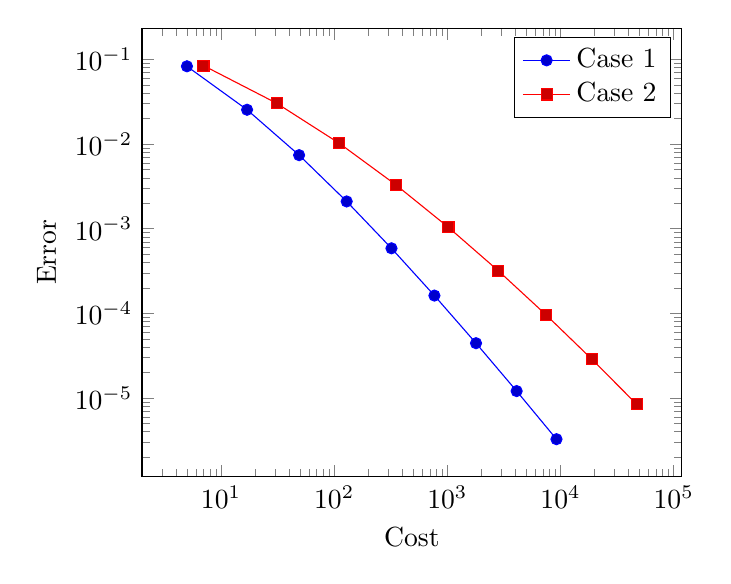
\begin{tikzpicture}
		\begin{loglogaxis}[xlabel=Cost,ylabel=Error]
		\addplot coordinates {
			(5,     8.31160034e-02)
			(17,    2.54685628e-02)
			(49,    7.40715288e-03)
			(129,   2.10192154e-03)
			(321,   5.87352989e-04)
			(769,   1.62269942e-04)
			(1793,  4.44248889e-05)
			(4097,  1.20714122e-05)
			(9217,  3.26101452e-06)
		};
		\addplot coordinates {
			(7,     8.47178381e-02)
			(31,    3.04409349e-02)
			(111,   1.02214539e-02)
			(351,   3.30346265e-03)
			(1023,  1.03886535e-03)
			(2815,  3.19646457e-04)
			(7423,  9.65789766e-05)
			(18943, 2.87339125e-05)
			(47103, 8.43749881e-06)
		};
		\legend{Case 1,Case 2}
		\end{loglogaxis}
	\end{tikzpicture}
	\caption{A larger example}
\end{figure}
\end{document}
\end{codeexample}

\item[Con{\TeX}t:] |\usemodule[pgfplots]| and

{\HEAD
\begin{codeexample}[code only]
\starttikzpicture
\startaxis
...
\stopaxis
\stoptikzpicture
\end{codeexample}
&
\begin{codeexample}[code only]
\starttikzpicture
\startsemilogxaxis
...
\stopsemilogxaxis
\stoptikzpicture
\end{codeexample}
\\
\end{tabular}%
}

A complete Con{\TeX}t--example file can be found in
\begin{codeexample}[code only]
doc/context/pgfplots/pgfplotsexample.tex.
\end{codeexample}

\item[plain \TeX:] |\input pgfplots.tex| and

{\HEAD
\begin{codeexample}[code only]
\tikzpicture
\axis
...
\endaxis
\endtikzpicture
\end{codeexample}
&
\begin{codeexample}[code only]
\tikzpicture
\semilogxaxis
...
\endsemilogxaxis
\endtikzpicture
\end{codeexample}
\\
\end{tabular}%
}

A complete plain--\TeX--example file can be found in
\begin{codeexample}[code only]
doc/plain/pgfplots/pgfplotsexample.tex.
\end{codeexample}
\end{description}

If you use |latex| / |dvips| or |pdflatex|, no further modifications are necessary. For |dvipdfm|, you should use the |\def\pgfsysdriver| line as indicated above in the examples (see also Section~\ref{sec:drivers}).


\subsection{A First Plot}
Plotting is done using |\begin{axis} ... \addplot ...; \end{axis}|, where |\addplot| is the main interface to perform plotting operations.
\begin{codeexample}[]
\begin{tikzpicture}
	\begin{axis}[
		xlabel=Cost,
		ylabel=Error]
	\addplot[color=red,mark=x] coordinates {
		(2,-2.8559703)
		(3,-3.5301677)
		(4,-4.3050655)
		(5,-5.1413136)
		(6,-6.0322865)
		(7,-6.9675052)
		(8,-7.9377747)
	};
	\end{axis}
\end{tikzpicture}
\end{codeexample}


\begin{codeexample}[]
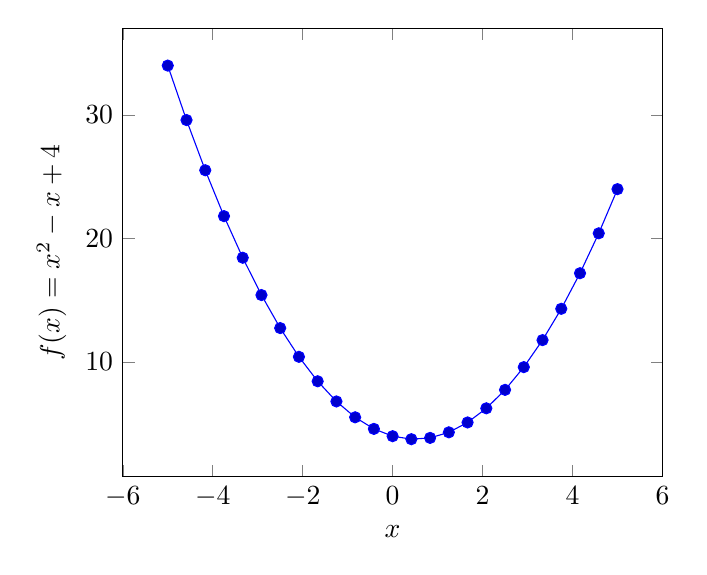
\begin{tikzpicture}
	\begin{axis}[
		xlabel=$x$,
		ylabel={$f(x) = x^2 - x +4$}
	]
	% use TeX as calculator:
	\addplot {x^2 - x +4};
	\end{axis}
\end{tikzpicture}
\end{codeexample}

\begin{codeexample}[]
\begin{tikzpicture}
	\begin{axis}[
		xlabel=$x$,
		ylabel=$\sin(x)$
	]
	% invoke external gnuplot as
	% calculator:
	\addplot gnuplot[id=sin]{sin(x)};
	\end{axis}
\end{tikzpicture}
\end{codeexample}

The |plot coordinates|, |plot expression| and |plot gnuplot| commands are three of the several supported ways to create plots, see Section~\ref{sec:addplot} for more details\footnote{Please note that you need \lstinline{gnuplot} installed to use \lstinline{plot gnuplot}.} and the remaining ones (|plot file|, |plot shell|, |plot table| and |plot graphics|). The options `|xlabel|' and `|ylabel|' define axis descriptions.

\subsection{Two Plots in the Same Axis}
Multiple |\addplot|-commands can be placed into the same axis, and a |cycle list| is used to automatically select different line styles:
	% generated with this statement:
	%\addplot plot[id=filesuffix_noise,domain=-6:5,samples=10] gnuplot{(-x**5 - 242 + (-300 + 600*rand(0)))};
\begin{codeexample}[leave comments]
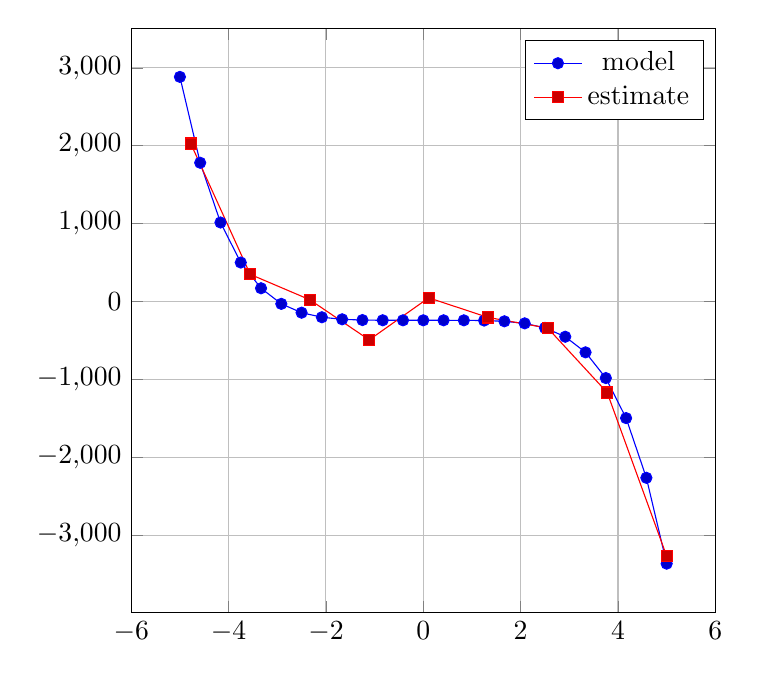
\begin{tikzpicture}
	\begin{axis}[
		height=9cm,
		width=9cm,
		grid=major,
	]
		
	\addplot {-x^5 - 242};
	\addlegendentry{model}

	\addplot coordinates {
		(-4.77778,2027.60977)
		(-3.55556,347.84069)
		(-2.33333,22.58953)
		(-1.11111,-493.50066)
		(0.11111,46.66082)
		(1.33333,-205.56286)
		(2.55556,-341.40638)
		(3.77778,-1169.24780)
		(5.00000,-3269.56775)
	};
	\addlegendentry{estimate}
	\end{axis}
\end{tikzpicture}
\end{codeexample}
A legend entry is generated if there are |\addlegendentry| commands (or one |\legend| command).

\subsection{Logarithmic Plots}
Logarithmic plots show $\log x$ versus $\log y$  (or just one logarithmic axis). \PGFPlots\ normally uses the natural logarithm, i.e. basis $e\approx2.718$ (see the key |log basis x|). Now, the axis description also contains minor ticks and the labels are placed at $10^i$.
\begin{codeexample}[]
\begin{tikzpicture}
\begin{loglogaxis}[xlabel=Cost,ylabel=Gain]
\addplot[color=red,mark=x] coordinates {
	(10,100)
	(20,150)
	(40,225)
	(80,340)
	(160,510)
	(320,765)
	(640,1150)
};
\end{loglogaxis}
\end{tikzpicture}
\end{codeexample}
A common application is to visualise scientific data. This is often provided in the format $1.42\cdot10^4$, usually written as 1.42e+04. Suppose we have a numeric table named |pgfplots.testtable|, containing
\begin{codeexample}[code only,tabsize=6]
Level Cost  Error
1     7     8.471e-02
2     31    3.044e-02
3     111   1.022e-02
4     351   3.303e-03
5     1023  1.038e-03
6     2815  3.196e-04
7     7423  9.657e-05
8     18943 2.873e-05
9     47103 8.437e-06
\end{codeexample}
\noindent then we can plot |Cost| versus |Error| using
\begin{codeexample}[]
\begin{tikzpicture}
\begin{loglogaxis}[
	xlabel=Cost,
	ylabel=Error]
\addplot[color=red,mark=x] coordinates {
	(5,    8.31160034e-02)
	(17,   2.54685628e-02)
	(49,   7.40715288e-03)
	(129,  2.10192154e-03)
	(321,  5.87352989e-04)
	(769,  1.62269942e-04)
	(1793, 4.44248889e-05)
	(4097, 1.20714122e-05)
	(9217, 3.26101452e-06)
};

\addplot[color=blue,mark=*] 
	table[x=Cost,y=Error] {pgfplots.testtable};

\legend{Case 1,Case 2}
\end{loglogaxis}
\end{tikzpicture}
\end{codeexample}
The first plot employs inline coordinates; the second one reads numerical data from file and plots column `|Cost|' versus `|Error|'.

\noindent
Besides the environment ``|loglogaxis|'' you can use
\begin{itemize}
	\item |\begin{axis}...\end{axis}| for normal plots,
	\item |\begin{semilogxaxis}...\end{semilogxaxis}| for plots which have a normal~$y$ axis and a logarithmic~$x$ axis,
	\item |\begin{semilogyaxis}...\end{semilogyaxis}| the same with $x$~and~$y$ switched,
	\item |\begin{loglogaxis}...\end{loglogaxis}| for double--logarithmic plots.
\end{itemize}
You can also use
\begin{codeexample}[code only]
\begin{axis}[xmode=normal,ymode=log]
...
\end{axis}
\end{codeexample}
which is the same as |\begin{semilogyaxis}...\end{semilogyaxis}|.
\begin{codeexample}[]
\begin{tikzpicture}
	\begin{semilogyaxis}[
		xlabel=Index,ylabel=Value]

	\addplot[color=blue,mark=*] coordinates {
		(1,8)
		(2,16)
		(3,32)
		(4,64)
		(5,128)
		(6,256)
		(7,512)
	};
	\end{semilogyaxis}%
\end{tikzpicture}%
\end{codeexample}

\subsection{Cycling Line Styles}
You can skip the style arguments for |\addplot[...]| to determine plot specifications from a predefined list:
\label{page:plotcoords:src}%
\pgfmanualpdflabel{\textbackslash plotcoords}{}%
\begin{codeexample}[width=4cm]
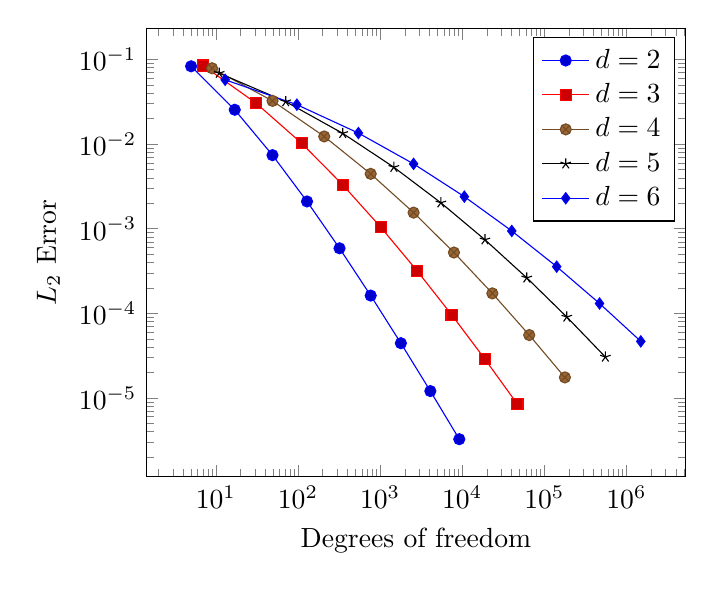
\begin{tikzpicture}
\begin{loglogaxis}[
	xlabel={Degrees of freedom},
	ylabel={$L_2$ Error}
]
\addplot coordinates {
	(5,8.312e-02)    (17,2.547e-02)   (49,7.407e-03)
	(129,2.102e-03)  (321,5.874e-04)  (769,1.623e-04)
	(1793,4.442e-05) (4097,1.207e-05) (9217,3.261e-06)
};

\addplot coordinates{
	(7,8.472e-02)    (31,3.044e-02)    (111,1.022e-02)
	(351,3.303e-03)  (1023,1.039e-03)  (2815,3.196e-04)
	(7423,9.658e-05) (18943,2.873e-05) (47103,8.437e-06)
};

\addplot coordinates{
	(9,7.881e-02)     (49,3.243e-02)    (209,1.232e-02)
	(769,4.454e-03)   (2561,1.551e-03)  (7937,5.236e-04)
	(23297,1.723e-04) (65537,5.545e-05) (178177,1.751e-05)
};

\addplot coordinates{
	(11,6.887e-02)    (71,3.177e-02)     (351,1.341e-02)
	(1471,5.334e-03)  (5503,2.027e-03)   (18943,7.415e-04)
	(61183,2.628e-04) (187903,9.063e-05) (553983,3.053e-05)
};

\addplot coordinates{
	(13,5.755e-02)     (97,2.925e-02)     (545,1.351e-02)
	(2561,5.842e-03)   (10625,2.397e-03)  (40193,9.414e-04)
	(141569,3.564e-04) (471041,1.308e-04) (1496065,4.670e-05)
};
\legend{$d=2$,$d=3$,$d=4$,$d=5$,$d=6$}
\end{loglogaxis}
\end{tikzpicture}
\end{codeexample}
\noindent
The |cycle list| can be modified, see the reference below.

\subsection{Scaling Plots}
You can use any of the \Tikz\ options to modify the appearance. For example, the ``|scale|'' transformation takes the picture as such and scales it (just like |\includegraphics|):

\begin{codeexample}[]
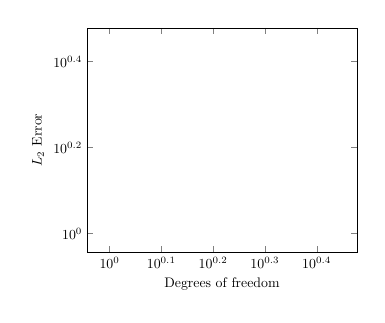
\begin{tikzpicture}[scale=0.5]
	\begin{loglogaxis}[
		xlabel={Degrees of freedom},
		ylabel={$L_2$ Error}
	]
	\plotcoords
	\legend{$d=2$,$d=3$,$d=4$,$d=5$,$d=6$}
	\end{loglogaxis}
\end{tikzpicture}

\begin{tikzpicture}[scale=1.1]
	\begin{loglogaxis}[
		xlabel={Degrees of freedom},
		ylabel={$L_2$ Error}
	]
	\plotcoords
	\legend{$d=2$,$d=3$,$d=4$,$d=5$,$d=6$}
	\end{loglogaxis}
\end{tikzpicture}
\end{codeexample}
However, you can also scale plots by assigning a |width=5cm| and/or |height=3cm| argument. This only affects the distance of point coordinates, no font sizes or axis descriptions:
\begin{codeexample}[]
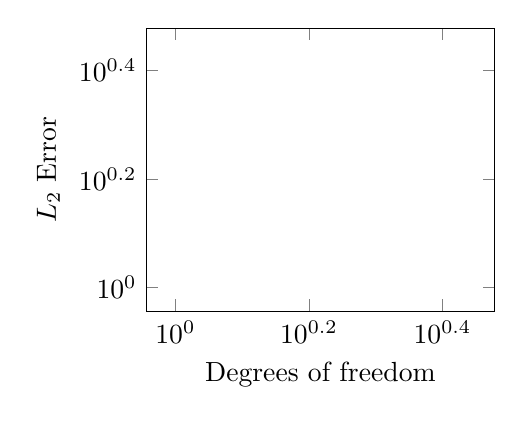
\begin{tikzpicture}
	\begin{loglogaxis}[
		width=6cm,
		xlabel={Degrees of freedom},
		ylabel={$L_2$ Error}
	]
	\plotcoords
	\legend{$d=2$,$d=3$,$d=4$,$d=5$,$d=6$}
	\end{loglogaxis}
\end{tikzpicture}

\begin{tikzpicture}
	\begin{loglogaxis}[
		width=8cm,
		xlabel={Degrees of freedom},
		ylabel={$L_2$ Error}
	]
	\plotcoords
	\legend{$d=2$,$d=3$,$d=4$,$d=5$,$d=6$}
	\end{loglogaxis}
\end{tikzpicture}
\end{codeexample}

Use the predefined styles |normalsize|, |small|, |footnotesize| to adopt font sizes and ticks automatically. Use the |/pgfplots/scale| key to rescale the axis without affecting fonts.

\endinput
%
%% main=manual.tex

\section{Command Reference}
\subsection{The axis-environments}
There is an axis environment for linear scaling, two for semi-logarithmic scaling and one for double-logarithmic scaling.
\begin{environment}{{axis}\marg{options}}
	The axis environment for normal plots with linear axis scaling.

	Use
\begin{codeexample}[code only]
\tikzstyle{every linear axis}+=[...]
\end{codeexample}
to install styles specifically for linear axes. These styles can contain both \Tikz- and \PGFPlots\ options.
\end{environment}

\begin{environment}{{semilogxaxis}\marg{options}}
The axis environment for logarithmic scaling of~$x$ and normal scaling of~$y$.
Use
\begin{codeexample}[code only]
\tikzstyle{every semilogx axis}+=[...]
\end{codeexample}
to install styles specifically for the case with \texttt{xmode=log}, \texttt{ymode=normal}.
\end{environment}

\begin{environment}{{semilogyaxis}\marg{options}}
The axis environment for normal scaling of~$x$ and logarithmic scaling of~$y$,
The style `\texttt{every semilogy axis}' will be installed for each such plot.
\end{environment}

\begin{environment}{{loglogaxis}\marg{options}}
The axis environment for logarithmic scaling of both, $x$~and~$y$ axes,
As for the other axis possibilities, there is a style `\texttt{every loglog axis}' which is installed at the environment's beginning.
\end{environment}

They are all equivalent to
\begin{codeexample}[code only]
\begin{axis}[
	xmode=log|normal,
	ymode=log|normal]
...
\end{axis}
\end{codeexample}
with properly set variables `\texttt{xmode}' and `\texttt{ymode}' (see below).

\subsection{The plot command}
\label{sec:addplot}%
\begin{command}{\addplot[\meta{style options}] \textcolor{gray}{plot[\meta{behavior options}]} \meta{input data} \meta{trailing path commands};}
This is the main plotting command, available within one of the plotting environments.

It reads point coordinates from one of the available input sources specified by \meta{input data}, updates limits, remembers \meta{style options} for use in a legend (if any) and applies any necessary coordinate transformations (or logarithms).

The \meta{style options} can be omitted in which case the next entry from the |cycle list| will be inserted as \meta{style options}. These keys characterize the plot's type like linear interpolation, smooth plot, constant interpolation or bar plot and define colors, markers and line specifications. 

Finally, if |\addplot| successfully processed all coordinates from \meta{input data}, it generates \Tikz-drawing commands (for example |plot coordinate {...}|). If \meta{trailing path commands} is not empty, these arguments are appended to the final drawing command.

\noindent
Some more details:
\begin{itemize}
	\item The style |/tikz/every axis plot| will be installed at the beginning of \meta{style options}. That means you can use
	\begin{codeexample}[code only]
	\tikzstyle{every axis plot}+=[...]
	\end{codeexample}
	to add options to all your plots. Furthermore, if you have more than one plot inside of an axis, you can also use
	\begin{codeexample}[code only]
	\tikzstyle{every axis plot no 3}+=[...]
	\end{codeexample}
	to modify options for the plot with number~$3$ only. The first plot has number~$0$.
	\item The \meta{style options} are remembered for the legend. Furthermore, they are available as `\texttt{current plot style}' as long as the path is not yet finished or in associated error bars.
	\item See subsection~\ref{sec:markers} for a list of available markers and line styles.
	\item For log plots, \PGFPlots\ will compute the natural logarithm $\log(\cdot)$ numerically. This works with normal fixed point numbers or in scientific notation. For example, the following numbers are valid input to \lstinline!\addplot!.
\begin{codeexample}[]
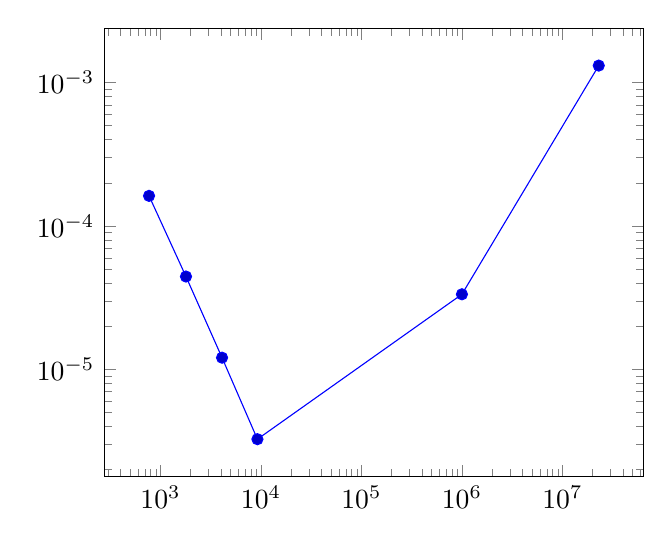
\begin{tikzpicture}
\begin{loglogaxis}
\addplot coordinates {
	(769,	1.6227e-04)
	(1793,	4.4425e-05)
	(4097,	1.2071e-05)
	(9217,	3.2610e-06)
	(1e6,	0.00003341)
	(2.3e7,	0.00131415)
};
\end{loglogaxis}
\end{tikzpicture}
\end{codeexample}
	You can represent arbitrarily small or very large numbers as long as its logarithm can be represented as a \TeX-length (up to about~$16384$). Of course, any coordinate~$x\le 0$ is not possible since the logarithm of a non-positive number is not defined. Such coordinates will be skipped automatically.

	\item For normal plots, \PGFPlots\ applies floating point arithmetics to support large or small numbers like 0.00000001234 or $1.234\cdot 10^{24}$. Its number range is very large because the parsing methods use \TeX's integers for exponents. The relative precision is at least~$5$ significant decimal digits for the mantisse. As soon as the axes limits are completely known, \PGFPlots\ applies a transformation which maps these floating point numbers into \TeX-precision using transformations
		\[ T_x(x) = 10^{s_x} \cdot x - a_x \text{ and } T_y(y) = 10^{s_y} \cdot y - a_y \]
	with properly chosen integers $s_x, s_y \in \Z$ and shifts $a_x,a_y\in \R$. This ensures invariance of axis ranges. See section~\ref{sec:disabledatascaling} for more details.

	\item As a consequence of the coordinate parsing routines, you can't use the mathematical expression parsing method of \PGF\ as coordinates (that means: you will need to provide coordinates without suffixes like ``cm'' or ``pt'' and you can't invoke mathematical functions).
	
	\item If you did not specify axis limits for $x$ and $y$ manually, \lstinline!\addplot! will compute them automatically. 
	The automatic computation of axis limits works as follows:
		\begin{enumerate}
			\item Every coordinate will be checked. Care has been taken to avoid \TeX's limited numerical capabilities.
			\item Since more than one \lstinline!\addplot! command may be used inside an \lstinline!\begin{axis}...\end{axis}!, all drawing commands will be postponed until \lstinline!\end{axis}!.
		\end{enumerate}
\end{itemize}
\end{command}

\begin{figure}
	\centering
	\tikzstyle{every picture}+=[baseline]%
	\tikzstyle{every axis}+=[width=6cm,anchor=north west,y label style={text width=0pt}]%
	\lstset{basicstyle=\ttfamily\footnotesize,aboveskip=0pt,belowskip=0pt}%
	\begin{tikzpicture}%
		\begin{pgfinterruptboundingbox}
		\begin{axis}[ymin=0,ymax=1,enlargelimits=false,name=an axis]
		\addplot[blue!80!black,fill=blue,fill opacity=0.5] coordinates 
			{(0,0.1) (0.1,0.15) (0.2,0.5) (0.3,0.62) (0.4,0.56) (0.5,0.58) (0.6,0.65) (0.7,0.6) (0.8,0.58) (0.9,0.55) (1,0.52)} 
		|- (axis cs:0,0) -- cycle;
		\addplot[red,fill=red!90!black,opacity=0.5] coordinates 
			{(0,0.25) (0.1,0.27) (0.2,0.24) (0.4,0.26) (0.5,0.3) (0.6,0.23) (0.7,0.2) (0.8,0.15) (0.9,0.1) (1,0.1)}
		 |- (axis cs:0,0) -- cycle;
		\addplot[green!20!black] coordinates
			{(0,0.4) (0.2,0.75) (1,0.75)};
		\end{axis}

		\begin{axis}[name=a second axis,at={(0,-4.5cm)}]
		\addplot plot[id=parable,domain=-5:5] function{4*x**2 - 5} node[pin=180:{$4x^2-5$}]{};
		\end{axis}
		\end{pgfinterruptboundingbox}
		\useasboundingbox (a second axis.below south west) (an axis.above north east);
	\end{tikzpicture}%
	\nobreak
	\hspace{10pt}%
	\nobreak
	\begin{minipage}[t]{8cm}%
	\vspace{0pt}%
\begin{codeexample}[code only]
\begin{axis}[ymin=0,ymax=1,enlargelimits=false]
\addplot
	[blue!80!black,fill=blue,fill opacity=0.5] 
coordinates
{(0,0.1)	(0.1,0.15)	(0.2,0.5)	(0.3,0.62)
 (0.4,0.56)	(0.5,0.58)	(0.6,0.65)	(0.7,0.6)
 (0.8,0.58) (0.9,0.55)	(1,0.52)} 
|- (axis cs:0,0) -- cycle;
\addplot
	[red,fill=red!90!black,opacity=0.5]
coordinates 
{(0,0.25)	(0.1,0.27)	(0.2,0.24)	(0.3,0.24)
 (0.4,0.26)	(0.5,0.3)	(0.6,0.23)	(0.7,0.2)
 (0.8,0.15)	(0.9,0.1)	(1,0.1)}
|- (axis cs:0,0) -- cycle;
\addplot[green!20!black] coordinates
	{(0,0.4) (0.2,0.75) (1,0.75)};
\end{axis}

\begin{axis}
\addplot plot
	[id=parable,domain=-5:5] 
	function{4*x**2 - 5} 
	node[pin=180:{$4x^2-5$}]{};
\end{axis}
\end{codeexample}
	\end{minipage}%
	\caption{Two examples of using \Tikz-paths after plotting commands.}
	\label{fig:after:paths}
\end{figure}

\begin{addplotoperation}[noindex]{coordinates}{\marg{coordinate sequence}}
The `\texttt{plot coordinates}' command is provided by \Tikz\ and reads its input data from a sequence of point coordinates.
\begin{codeexample}[code only]
\addplot plot coordinates {
	(0,0)
	(0.5,1)
	(1,2)
};
\end{codeexample}

You can also supply error coordinates (reliability bounds) if you are interested in error bars. Simply append the error coordinates with `\texttt{+- (ex,ey)}' to the associated coordinate:
\begin{codeexample}[code only]
\addplot plot coordinates {
	(0,0) +- (0.1,0)
	(0.5,1) +- (0.4,0.2)
	(1,2)
	(2,5) +- (1,0.1)
};
\end{codeexample}
or 
\begin{codeexample}[code only]
\addplot plot coordinates {
	(1300,1e-6) +- (0.1,0.2)
	(2600,5e-7) +- (0.2,0.5)
	(4000,1e-7) +- (0.1,0.01)
};
\end{codeexample}
These error coordinates are only used in case of error bars, see section~\ref{sec:errorbars}. You will also need to configure whether these values denote absolute or relative errors.

The coordinates as such can be numbers as |+5|, |-1.2345e3|, |35.0e2|, |0.00000123| or |1e2345e-8|. They are not limited to \TeX's precision.
\end{addplotoperation}


\begin{addplotoperation}[noindex]{file}{\marg{name}}
\PGFPlots\ supports two ways to read plot coordinates of external files, and one of them is the \Tikz-command `\texttt{plot file}'. It is to be used like
\begin{codeexample}[code only]
\addplot plot file {datafile.dat};
\end{codeexample}
where \marg{name} is a text file with at least two columns which will be used as $x$ and $y$ coordinates. Such files are often generated by \textsc{gnuplot}:
\begin{codeexample}[code only]
#Curve 0, 20 points
#x y type
0.00000 0.00000 i
0.52632 0.50235 i
1.05263 0.86873 i
1.57895 0.99997 i
...
9.47368 -0.04889 i
10.00000 -0.54402 i
\end{codeexample}
This listing has been copied from~\cite[section~16.4]{tikz}. The mentioned section also contains some more details about using \texttt{plot file}.
\end{addplotoperation}

\begin{addplotoperation}[noindex]{function}{\marg{gnuplot code}}
The plot function command uses the external program \texttt{gnuplot} to compute coordinates. The resulting coordinates are written to a text file which will be plotted with \texttt{plot file}. \PGF\ checks whether coordinates need to be re-generated and calls \texttt{gnuplot} whenever necessary (this is usually the case if you change the number of samples, the argument to \texttt{plot function} or the plotted domain\footnote{Please note that \PGFPlots\ produces slightly different files than \Tikz\ when used with \texttt{plot function} (it configures high precision output). You should use different ids to avoid conflicts in such a case.}).

The \meta{style options} determine the appearance of the plotted function; these parameters also affect the legend. The \meta{behavior options} are specific to the gnuplot interface. These options are described in all detail in \cite[section~18.6]{tikz}. Summary:
\begin{description}
\item[\texttt{/tikz/domain=[start:end]}] Determines the plotted range. This is not necessarily the same as the axis limits (which are configured with the \texttt{xmin}/\texttt{xmax} options). 
\item[\texttt{/tikz/id=<id>}] A unique identifier for the current plot. It is used to generate temporary filenames for gnuplot output.
\item[\texttt{/tikz/prefix=<prefix>}] A common path prefix for temporary filenames (see \cite[section~18.6]{tikz} for details).
\item[\texttt{/tikz/samples=<number>}] Sets the number of sample points.
\item[\texttt{/tikz/raw gnuplot}] Disables the use of samples and domains.
\end{description}
\begin{codeexample}[]
\begin{tikzpicture}
\begin{axis}
\addplot plot[id=sin] function{sin(x)};
\end{axis}
\end{tikzpicture}
\end{codeexample}
\begin{codeexample}[]
\begin{tikzpicture}
\begin{semilogyaxis}
\addplot plot[id=exp,domain=0:10] function{exp(x)};
\end{semilogyaxis}
\end{tikzpicture}
\end{codeexample}
Please refer to \cite[section~18.6]{tikz} for more details.
\end{addplotoperation}

\begin{addplotoperation}[noindex]{table}{[\meta{source columns}]\marg{filename}}
\PGFPlots\ comes with a new plotting command, the `\texttt{plot table}' macro. It's usage is similar in spirit to `\texttt{plot file}', but its flexibility is higher. Given a data file like
\begin{lstlisting}[tabsize=8]
dof	L2		Lmax		maxlevel
5	8.31160034e-02	1.80007647e-01	2
17	2.54685628e-02	3.75580565e-02	3
49	7.40715288e-03	1.49212716e-02	4
129	2.10192154e-03	4.23330523e-03	5
321	5.87352989e-04	1.30668515e-03	6
769	1.62269942e-04	3.88658098e-04	7
1793	4.44248889e-05	1.12651668e-04	8
4097	1.20714122e-05	3.20339285e-05	9
9217	3.26101452e-06	8.97617707e-06	10
\end{lstlisting}
one may want to plot `\texttt{dof}' versus `\texttt{L2}' or `\texttt{dof}' versus `\texttt{Lmax}'. This can be done by
\begin{codeexample}[code only]
\begin{tikzpicture}
	\begin{loglogaxis}[
		xlabel=Dof,
		ylabel=$L_2$ error$]
	\addplot table[x=dof,y=L2] {datafile.dat};
	\end{loglogaxis}
\end{tikzpicture}
\end{codeexample}
or
\begin{codeexample}[code only]
\begin{tikzpicture}
	\begin{loglogaxis}[
		xlabel=Dof,
		ylabel=$L_infty$ error$]
	\addplot table[x=dof,y=Lmax] {datafile.dat};
	\end{loglogaxis}
\end{tikzpicture}
\end{codeexample}
Alternatively, you can load the table \emph{once} and use it \emph{multiple} times:
\begin{codeexample}[code only]
\pgfnumtableread{datafile.dat} to \table
...
\addplot table[x=dof,y=L2] from \table;
...
\addplot table[x=dof,y=Lmax] from \table;
...
\end{codeexample}
I am not really sure how much time can be saved, but it works anyway.

If you do prefer to access columns by column indices instead of column names (or your tables do not have table names), you can also use
\begin{codeexample}[code only]
\addplot table[x index=2,y index=3] {datafile.dat};
\addplot table[x=dof,y index=2] {datafile.dat};
\end{codeexample}

Summary and remarks:
\begin{itemize}
	\item Use \texttt{plot table[x=\marg{column name},y=\marg{column name}]} to access column names. Those names are case sensitive and need to exist.
	\item Use \texttt{plot table[x index=\marg{column index},y index=\marg{column index}]} to access column indices. Indexing starts with~$0$. You may also use an index for~$x$ and a column name for~$y$.
	\item Use \texttt{plot table[header=false] \marg{file name}} if your input file has no column names. Otherwise, the first non-comment line is checked for column names: if all entries are numbers, they are treated as numerical data; if one of them is not a number, all are treated as column names.
	\item It is possible to read error coordinates from tables as well. Simply add options `\texttt{x error}', `\texttt{y error}' or `\texttt{x error index}'/`\texttt{y error index}' to \marg{source columns}. See section~\ref{sec:errorbars} for details about error bars.
	\item Use \texttt{plot table[\meta{source columns}] from \textbackslash macro} to use a pre--read table. Tables can be read using
\begin{codeexample}[code only]
\pgfnumtableread{datafile.dat} to \macroname.
\end{codeexample}
	\item The accepted input format is as follows:
		\begin{itemize}
			\item Columns are separated by white spaces.
			\item Any line starting with `\#' or `\%' is ignored.
			\item The first line will be checked if it contains numerical data. If there is a column in the first line which is \emph{no} number, the complete line is considered to be a header which contains column names. Otherwise it belongs to the numerical data and you need to access column indices instead of names.

			\item There is future support for a second header line which must start with `\texttt{\$flags}'. Currently, such a line is ignored. It may be used to provide number formatting hints like precision and number format if those tables shall be typeset inside of \TeX.
			\item The accepted number format is the same as for `\texttt{plot coordinates}', see above.
			\item If you omit column selectors, the default is to plot the first column against the second. That means \texttt{plot table} does exactly the same job as \texttt{plot file} for this case.
		\end{itemize}
\end{itemize}
\end{addplotoperation}


\begin{command}{\addplot+[\meta{style options}] \textcolor{gray}{\dots};}
Does the same like \texttt{\textbackslash addplot[\meta{style options}] ...;} except that \meta{style options} is \emph{appended} to the arguments which would have been taken for \lstinline!\addplot ...! (the element of the default list).

\begin{codeexample}[]
\begin{tikzpicture}
\begin{axis}
\addplot coordinates {(0,0) (0.5,0.5) (1,1)};
\end{axis}
\end{tikzpicture}

\begin{tikzpicture}
\begin{axis}
\addplot+[only marks] coordinates {(0,0) (0.5,0.5) (1,1)};
\end{axis}
\end{tikzpicture}
\end{codeexample}
\end{command}

\subsection{Accessing axis coordinates with \texttt{axis cs}}
\label{sec:axis:coords}%
\begin{coordinatesystem}{axis cs}
\PGFPlots\ provides a new coordinate system for use inside of an axis, the ``axis coordinate system'', \texttt{axis cs}.

It can be used to draw any \Tikz-graphics at axis coordinates. It is used like
\begin{codeexample}[code only]
\draw 
	(axis cs:18943,2.873391e-05) 
|-	(axis cs:47103,8.437499e-06);
\end{codeexample}
\begin{codeexample}[]
\tikzstyle{every pin}=[fill=white,
	draw=black,
	font=\footnotesize]
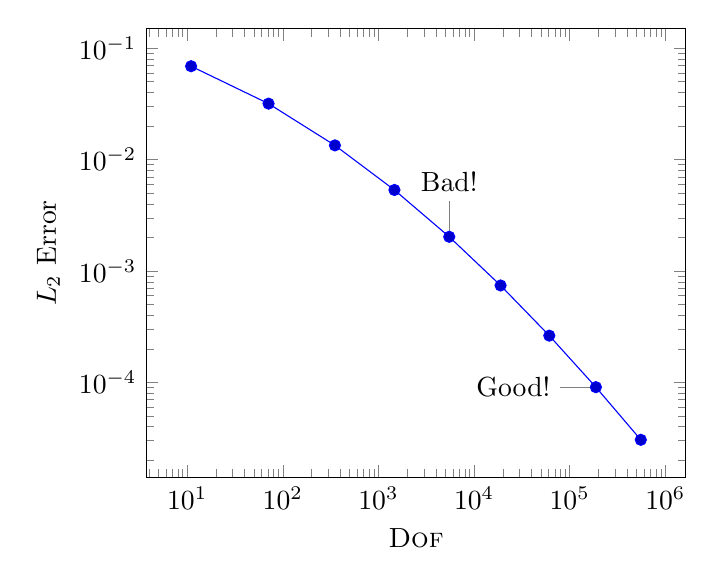
\begin{tikzpicture}
	\begin{loglogaxis}[
		xlabel={\textsc{Dof}},
		ylabel={$L_2$ Error}
	]

	\addplot coordinates {
		(11,	6.887e-02)
		(71,	3.177e-02)
		(351,	1.341e-02)
		(1471,	5.334e-03)
		(5503,	2.027e-03)
		(18943,	7.415e-04)
		(61183,	2.628e-04)
		(187903,	9.063e-05)
		(553983,	3.053e-05)
	};

	\node[coordinate,pin=above:Bad!] 
		at (axis cs:5503,2.027e-03) {};
	\node[coordinate,pin=left:Good!] 
		at (axis cs:187903,9.063e-05)	{};
	\end{loglogaxis}
\end{tikzpicture}
\end{codeexample}

\begin{codeexample}[]
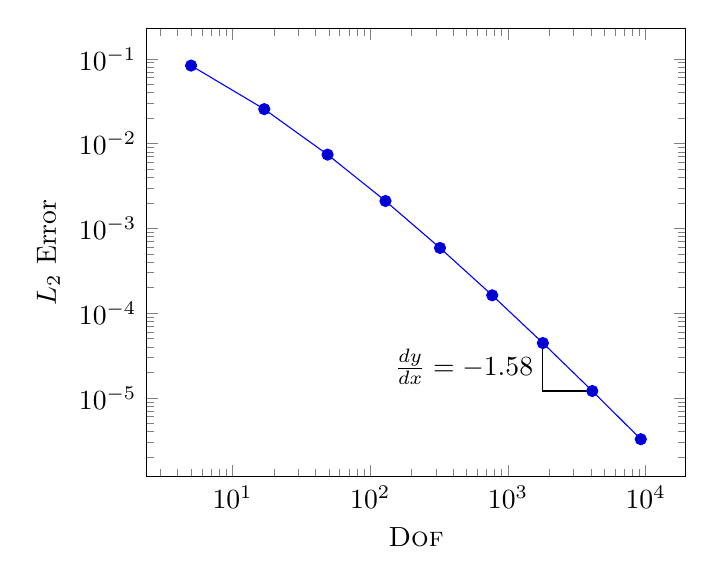
\begin{tikzpicture}
\begin{loglogaxis}[
	xlabel=\textsc{Dof},
	ylabel=$L_2$ Error
]
\draw 
		(axis cs:1793,4.442e-05)
	|-	(axis cs:4097,1.207e-05)
	node[near start,left] 
	{$\frac{dy}{dx} = -1.58$};

\addplot coordinates {
	(5,		8.312e-02)
	(17,	2.547e-02)
	(49,	7.407e-03)
	(129,	2.102e-03)
	(321,	5.874e-04)
	(769,	1.623e-04)
	(1793,	4.442e-05)
	(4097,	1.207e-05)
	(9217,	3.261e-06)
};
\end{loglogaxis}
\end{tikzpicture}
\end{codeexample}

\paragraph{Attention:} Whenever you draw additional graphics, consider using \texttt{axis cs}! It applies any logarithms, data scaling transformations or whatever \PGFPlots\ usually does!
\end{coordinatesystem}

\subsection{Legend commands}

\begin{command}{\addlegendentry\marg{name}}
Adds a single legend entry to the legend list. This will also enable legend drawing.
\begin{codeexample}[]
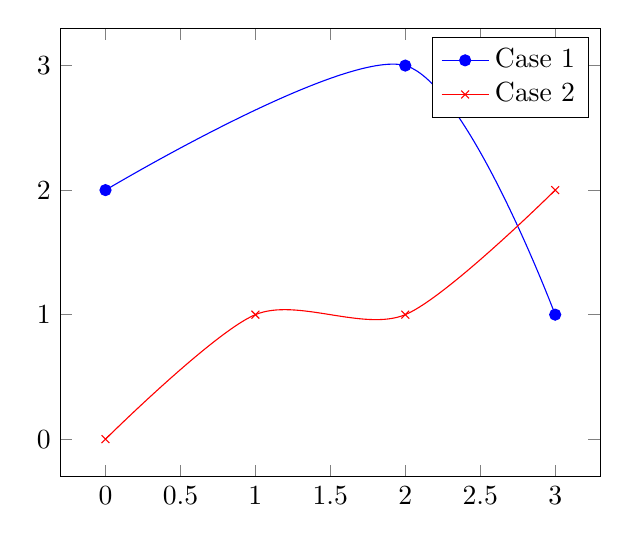
\begin{tikzpicture}
\begin{axis}
\addplot[smooth,mark=*,blue] coordinates {
	(0,2)
	(2,3)
	(3,1)
};
\addlegendentry{Case 1}

\addplot[smooth,color=red,mark=x]
	coordinates {
		(0,0)
		(1,1)
		(2,1)
		(3,2)
	};
\addlegendentry{Case 2}
\end{axis}
\end{tikzpicture}
\end{codeexample}
It does not matter where |\addlegendentry| commands are placed, only the sequence matters. You will need one |\addlegendentry| for every |\addplot| command.

There is limited support to change options for single legend entries using |\addlegendentry|[\meta{key-value-list}]|{...}|.
\end{command}



\label{sec:legenddef}%
\begin{command}{\legend\marg{list}}
You can use |\legend|\marg{list} to assign a complete legend.
\begin{codeexample}[code only]
\legend{$d=2$,$d=3$,$d=4$,$d=5$,$d=6$}
\end{codeexample}
The argument of |\legend| is a comma--separated list of entries, one for each plot. It is processed using the \PGF-foreach command\footnote{Older versions of \PGFPlots\ used \texttt{\textbackslash legend\{first\textbackslash\textbackslash second\textbackslash\textbackslash third\textbackslash\textbackslash\}} instead of comma--separated lists. This syntax is still accepted.}.
The short marker/line combination shown in legends is acquired from the \marg{style options} argument of |\addplot|.
\end{command}

\subsubsection{Legend appearance}
{%
\tikzstyle{every axis}+=[width=3cm,scale only axis,legend style={font=\footnotesize}]%
\begin{stylekey}{/tikz/every axis legend}
The style ``\texttt{every axis legend}'' determines the legend's position and outer appearance:
\begin{codeexample}[code only]
\tikzstyle{every axis legend}+=[
		at={(0,0)},
		anchor=south west]
\end{codeexample}
will draw it at the lower left corner of the axis while
\begin{codeexample}[code only]
\tikzstyle{every axis legend}+=[
		at={(1,1)},
		anchor=north east]
\end{codeexample}
means the upper right corner. The `\texttt{anchor}' option determines which point \emph{of the legend} will be placed at $(0,0)$ or $(1,1)$.

The legend is a \Tikz-matrix, so you can use any \Tikz\ option which affects
nodes and matrizes (see~\cite[section 13~and~14]{tikz}). The matrix is created by something like
\begin{codeexample}[code only]
\matrix[style=every axis legend] {
	draw plot specification 1 & \node{legend 1}\\
	draw plot specification 2 & \node{legend 2}\\
	...
};
\end{codeexample}
You can configure the number of horizontal legend entries with the axis-option ``\texttt{legend columns=\marg{number}}''.
\begin{codeexample}[]
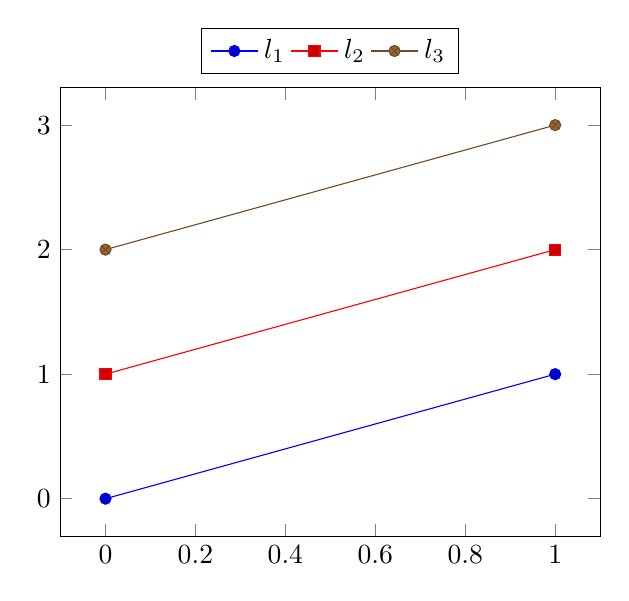
\begin{tikzpicture}
\begin{axis}[legend columns=4,
	legend style={at={(0.5,1.03)},
	anchor=south}]
\addplot coordinates {(0,0) (1,1)};
\addplot coordinates {(0,1) (1,2)};
\addplot coordinates {(0,2) (1,3)};
\legend{$l_1$,$l_2$,$l_3$}
\end{axis}
\end{tikzpicture}
\end{codeexample}
The example above uses |legend style| which is quite the same as |\tikzstyle{every axis legend}+=[...]|.

\begin{codeexample}[]
\tikzstyle{every axis legend}+=[
		at={(1.02,1)},
		anchor=north west]
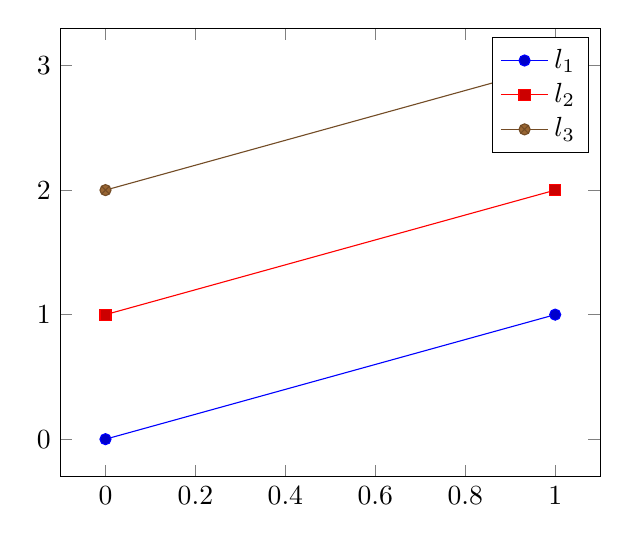
\begin{tikzpicture}
\begin{axis}
\addplot coordinates {(0,0) (1,1)};
\addplot coordinates {(0,1) (1,2)};
\addplot coordinates {(0,2) (1,3)};
\legend{$l_1$,$l_2$,$l_3$}
\end{axis}
\end{tikzpicture}
\end{codeexample}

\begin{codeexample}[]
\tikzstyle{every axis legend}+=[
		at={(1,0.5)},
		anchor=east]
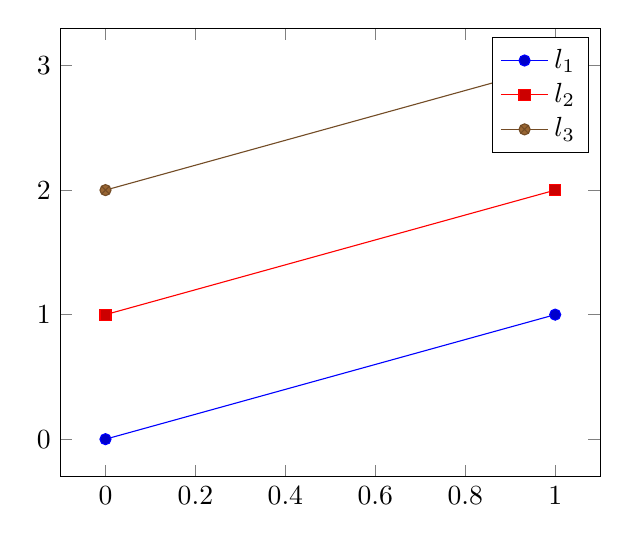
\begin{tikzpicture}
\begin{axis}
\addplot coordinates {(0,0) (1,1)};
\addplot coordinates {(0,1) (1,2)};
\addplot coordinates {(0,2) (1,3)};
\legend{$l_1$,$l_2$,$l_3$}
\end{axis}
\end{tikzpicture}
\end{codeexample}

\noindent
The default is
\begin{codeexample}[code only]
\tikzstyle{every axis legend}=[%
	cells={anchor=center},
	inner xsep=3pt,inner ysep=2pt,nodes={inner sep=2pt,text depth=0.15em},
	anchor=north east,%
	shape=rectangle,%
	fill=white,%
	draw=black,
	at={(0.98,0.98)}
]
\end{codeexample}
\paragraph{Attention:} you should \emph{not reset} the default style to stay compatible with future versions. If possible, use
\begin{codeexample}[code only]
\tikzstyle{every axis legend}+=[...]
\end{codeexample}
\end{stylekey}

}


\begin{command}{\autoplotspeclist}
This command should no longer be used, although it will be kept as technical implementation detail. Please use the `\texttt{cycle list}' option, section~\ref{sec:cycle:list}.
\end{command}

\begin{command}{\pgfmathlogtologten\meta{number}}
Assigns the result of $\meta{number}/\log(10)$ to \lstinline!\pgfmathresult!.
\end{command}

\begin{command}{\logten}
Expands to the constant $\log(10)$. Useful for logplots because $\log(10^i) = i\log(10)$. This command is only available inside of an \Tikz-picture.
\end{command}

\begin{command}{\pgfmathprintnumber\marg{number}}
Generates pretty--printed output\footnote{This method was previously \texttt{\textbackslash prettyprintnumber}. It's functionality has been included into \PGF\ and \texttt{\textbackslash prettyprintnumber} is now deprecated.} for the number \texttt{NUM}. This method is used for every tick label.

The number is printed using the current number printing options, see section~\ref{sec:number:printing} for the different number styles, rounding precision and rounding methods.
\end{command}

\subsection{Closing plots}
\begin{command}{\closedcycle}
	FIXME
\end{command}


\section{Option Reference}
There are several required and even more optional arguments to modify axes. They are used like
\begin{codeexample}[code only]
\begin{tikzpicture}
\begin{axis}[key=value,key2=value2]
...
\end{axis}
\end{tikzpicture}
\end{codeexample}
The overall appeareance can be changed with
\begin{codeexample}[code only]
\tikzstyle{every axis}+=[line width=1pt]
\end{codeexample}
for example. There are several other styles predefined to modify the appearance, see section~\ref{sec:styles}.

All \PGFPlots-options have the {\PGF}keys \emph{full key prefix}
\begin{codeexample}[code only]
/pgfplots/...
\end{codeexample}
Only the `\texttt{every ...}' styles have the full key prefix `\texttt{/tikz/every ...}' to maintain compatibility with `\lstinline!\tikzstyle!'.

\subsection{Axis options and \Tikz\ options}
You can mix \Tikz\ options and axis options inside of the axis arguments and in any of the axis--styles. For example,
\begin{codeexample}[code only]
\tikzstyle{every axis legend}+=[
	legend columns=3,font=\Large]
\end{codeexample}
assigns the `\texttt{legend columns}' option (an axis option) and will use `\texttt{font}' for drawing the legend (a \Tikz\ option).

The axis environments will process any known axis options, and all `\texttt{every}'--styles will be parsed for axis options. Every unknown option is supposed to be a \Tikz\ option and will be forward to the associated \Tikz\ drawing commands. For example, the `\lstinline{font=\Large}' above will be used as argument to the legend matrix, and the `\lstinline{font=\Large}' argument in 
\begin{codeexample}[code only]
\tikzstyle{every axis label}+=[
	ylabel=Error,xlabel=Dof,font=\Large}
\end{codeexample}
will be used in the nodes for axis labels (but not the axis title, for example).

It is an error if you assign incompatible options to axis labels, for example `\texttt{xmin}' and `\texttt{xmax}' can't be set inside of `\texttt{every axis label}'.

\paragraph{Remark:} \PGFPlots\ separates its own options from those of \Tikz. Misspelled options lead to \Tikz\ error messages. This has the unfortunate side effect that you need the \PGF\ 2.0-key syntax
\begin{codeexample}[code only]
\pgfkeys{/pgfplots/<own style name>/.style=
	{<style variables>}}
\end{codeexample}
instead of
\begin{codeexample}[code only]
\tikzstyle{<own style name>}=[<style variables>].
\end{codeexample}
Please refer to section~\ref{sec:styles:own} for more details.



\subsection{Plot Types}
\PGFPlots\ supports several two-dimensional line-plots like piecewise linear line plots, piecewise constant plots, smoothed plots, bar plots and comb plots. Most of them use the \PGF\ plot handler library directly, see \cite[section 18.8]{tikz}.

Plot types are part of the plot style, so they are set with options. The following list contains a short summary of \cite[section 18.8]{tikz}.


\subsubsection{Linear plots}
\begin{plottype}{sharp plot}
Linear (`sharp') plots are the default. Point coordinates are simply connected by straight lines. 
\begin{codeexample}[]
\begin{tikzpicture}
\begin{axis}
	\addplot+[sharp plot] coordinates {(0,0) (1,2) (2,3)};
\end{axis}
\end{tikzpicture}
\end{codeexample}

The `\texttt{+}' here means to use the normal plot cycle list and append `\texttt{sharp plot}' to its option list.
\end{plottype}

\subsubsection{Smooth plots}
\begin{plottype}{smooth}
Smooth plots interpolate smoothly between successive points.
\begin{codeexample}[]
\begin{tikzpicture}
\begin{axis}
	\addplot+[smooth] coordinates {(0,0) (1,2) (2,3)};
\end{axis}
\end{tikzpicture}
\end{codeexample}
\end{plottype}

\subsubsection{Constant plots}
Constant plots draw lines parallel to the $x$-axis to connect coordinates. The discontinuos edges may be drawn or not, and marks may be placed on left or right ends.

\begin{plottype}{const plot}
Connects all points with horizontal and vertical lines. Marks are placed left-handed on horizontal line segments, causing the plot to be right-sided continuous at all data points.

\begin{codeexample}[]
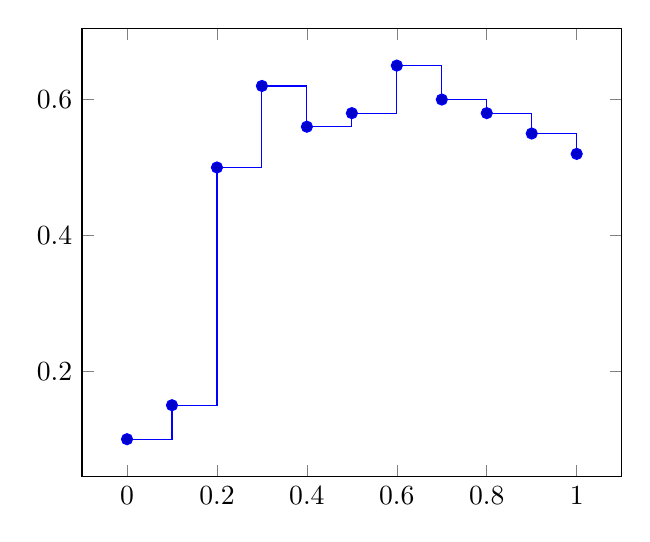
\begin{tikzpicture}
\begin{axis}
\addplot+[const plot]
coordinates
{(0,0.1)	(0.1,0.15)	(0.2,0.5)	(0.3,0.62)
 (0.4,0.56)	(0.5,0.58)	(0.6,0.65)	(0.7,0.6)
 (0.8,0.58) (0.9,0.55)	(1,0.52)};
\end{axis}
\end{tikzpicture}
\end{codeexample}


\begin{codeexample}[]
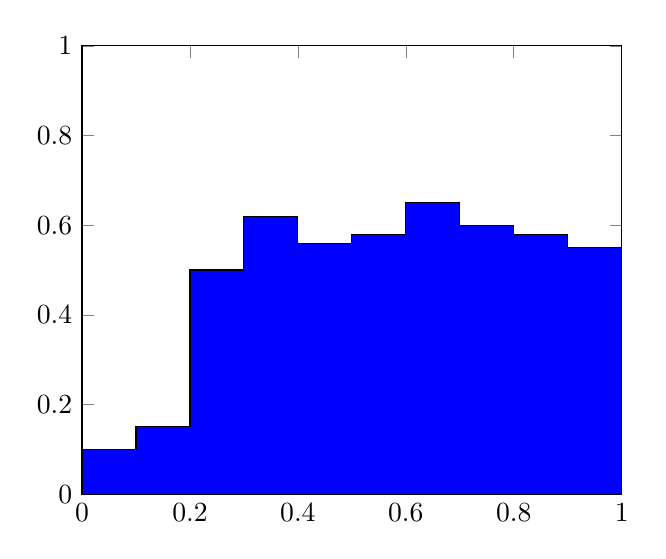
\begin{tikzpicture}
\begin{axis}[ymin=0,ymax=1,enlargelimits=false]
\addplot
	[const plot,fill=blue,draw=black] 
coordinates
{(0,0.1)	(0.1,0.15)	(0.2,0.5)	(0.3,0.62)
 (0.4,0.56)	(0.5,0.58)	(0.6,0.65)	(0.7,0.6)
 (0.8,0.58) (0.9,0.55)	(1,0.52)} 
	\closedcycle;
\end{axis}
\end{tikzpicture}
\end{codeexample}
\end{plottype}

\begin{plottype}{const plot mark left}
An alias for `\texttt{const plot}'.
\end{plottype}

\begin{plottype}{const plot mark right}
 A variant which places marks on the right of each line segment, causing plots to be left-sided continuous at coordinates.
\begin{codeexample}[]
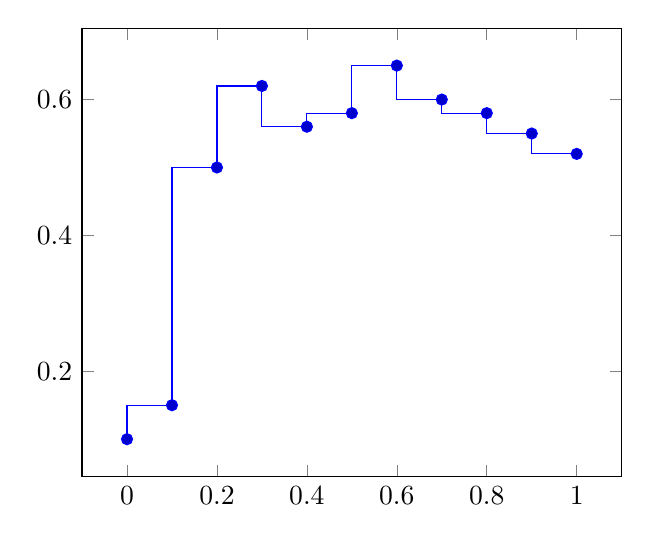
\begin{tikzpicture}
\begin{axis}
\addplot+[const plot mark right]
coordinates
{(0,0.1)	(0.1,0.15)	(0.2,0.5)	(0.3,0.62)
 (0.4,0.56)	(0.5,0.58)	(0.6,0.65)	(0.7,0.6)
 (0.8,0.58) (0.9,0.55)	(1,0.52)};
\end{axis}
\end{tikzpicture}
\end{codeexample}
\end{plottype}

\begin{plottype}{jump mark left}
A variant of `\texttt{const plot mark left}' which does not draw vertical lines.
\begin{codeexample}[]
\begin{tikzpicture}[samples=8]
\begin{axis}
\addplot+[jump mark left] 
	plot[id=parablex,domain=-5:0] 
	function{4*x**2 - 5};

\addplot+[jump mark right] 
	plot[id=cubic,domain=-5:0] 
	function{0.7*x**3 + 50};
\end{axis}
\end{tikzpicture}
\end{codeexample}
\end{plottype}

\begin{plottype}{jump mark right}
A variant of `\texttt{const plot mark right}' which does not draw vertical lines.
\end{plottype}

\subsubsection{Bar plots}
Bar plots place horizontal or vertical bars at coordinates. Multiple bar plots in one axis can be stacked on top of each other or aligned next to each other.

\begin{plottype}{xbar}
	Places horizontal bars between the $(y=0)$ line and each coordinate.
\begin{codeexample}[]
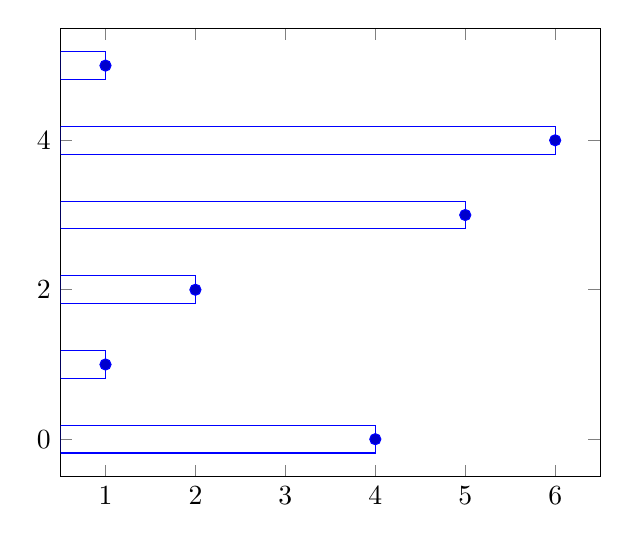
\begin{tikzpicture}
\begin{axis}
\addplot+[xbar] coordinates 
	{(4,0) (1,1) (2,2) 
	 (5,3) (6,4) (1,5)};
\end{axis}
\end{tikzpicture}
\end{codeexample}
	Bars are centered at plot coordinates with width |bar width|. Using bar plots usually means more than just a different way of how to connect coordinates, for example to draw ticks outside of the axis, change the legend's appearance or introduce shifts if multiple |\addplot| commands appear.

	There is a preconfigured style for |xbar| which is installed automatically if you provide |xbar| as argument to the axis environment which provides this functionality.
\begin{codeexample}[]
\begin{tikzpicture}
\begin{axis}[xbar,enlargelimits=0.15]
\addplot
[draw=blue,pattern=horizontal lines light blue] 
coordinates
	{(10,5) (15,10) (5,15) (24,20) (30,25)};

\addplot
[draw=black,pattern=horizontal lines dark blue] 
coordinates 
	{(3,5) (5,10) (15,15) (20,20) (35,25)};
\end{axis}
\end{tikzpicture}
\end{codeexample}
Here |xbar| yields |/pgfplots/xbar| because it is an argument to the axis, not to a single plot.

	Besides line-, fill- and colorstyles, bars can be configured with |bar width| and |bar shift|, see below.
\end{plottype}

\begin{stylekey}{/pgfplots/xbar=\marg{shift for multiple plots} (default 2pt)}
	This style sets several |/tikz/xbar| \emph{and} some commonly used options concerning horizontal bars. This is automatically done if you provide |xbar| as argument to an axis argument, see above.

The |xbar| style defines shifts if multiple plots are placed into one axis. If draws bars adjacent to each other, separated by \marg{shift for multiple plots}.

The style is defined as follows.
\begin{codeexample}[code only]
/pgfplots/xbar/.style={
	tick align=outside,
	/pgfplots/legend image code/.code=
		{\draw[##1,bar width=3pt,yshift=-0.2em,bar shift=0pt]
			plot coordinates {(0cm,0.8em) (2*\pgfplotbarwidth,0.6em)};},
	/pgf/bar shift={%
			-0.5*(\numplots*\pgfplotbarwidth + (\numplots-1)*#1)  + 
			(.5+\plotnum)*\pgfplotbarwidth + \plotnum*#1},
	/tikz/xbar},
\end{codeexample}
The formular for |bar shift| assigns shifts dependend on the total number of plots and the current plot's number. It is designed to fill a total width of $n \cdot $|bar width|$ + (n-1) \cdot $\marg{shift for multiple plots}. The $0.5$ compensates for centering.
\end{stylekey}

\begin{plottype}{ybar}
	Draws vertical bars between the ($x=0$) line and each input coordinate.
\begin{codeexample}[]
\begin{tikzpicture}
\begin{axis}
\addplot+[ybar] plot coordinates
	{(0,3) (1,2) (2,4) (3,1) (4,2)};
\end{axis}
\end{tikzpicture}
\end{codeexample}
	The example above simply changes how input coordinates shall be visualized. As mentioned for |xbar|, one usually needs modified legends and shifts for multiple bars in the same axis.

	There is a predefined style which installs these customizations when provided to the axis-environment:
\begin{codeexample}[]
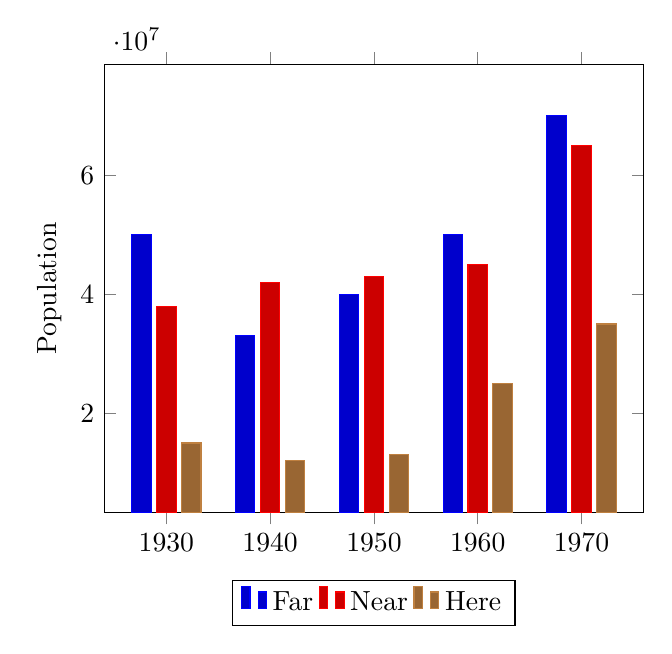
\begin{tikzpicture}
\begin{axis}[
	x tick label style={
		/pgf/number format/set thousands separator=},
	ylabel=Population,
	enlargelimits=0.15,
	legend style={at={(0.5,-0.15)},
		anchor=north,legend columns=-1},
	ybar,
	bar width=7pt,
]
\addplot[draw=blue,fill=blue!80!black] 
	coordinates {(1930,50e6) (1940,33e6)
		 (1950,40e6) (1960,50e6) (1970,70e6)};

\addplot[red,fill=red!80!black] 
	coordinates {(1930,38e6) (1940,42e6) 
		(1950,43e6) (1960,45e6) (1970,65e6)};

\addplot[brown,fill=brown!80!black] 
	coordinates {(1930,15e6) (1940,12e6) 
		(1950,13e6) (1960,25e6) (1970,35e6)};
\legend{Far,Near,Here}
\end{axis}
\end{tikzpicture}
\end{codeexample}
Here |ybar| yields |/pgfplots/ybar| because it is an argument to the axis, not to a single plot.

	As for |xbar|, the bar width and shift can be configured with |bar width| and |bar shift|.
\end{plottype}

\begin{stylekey}{/pgfplots/ybar=\marg{shift for multiple plots} (default 2pt)}
	As |/pgfplots/xbar|, this style sets the |/tikz/ybar| option to draw vertical bars, but it also provides commonly used options for vertical bars.

	If you supply |ybar| to an axis environment, |/pgfplots/ybar| will be chosen instead of |/tikz/ybar|.

	It changes the legend, draws ticks outside of the axis lines and draws multiple |\addplot| arguments adjacent to each other; block--centered at the $x$ coordinate and separated by \marg{shift for multiple plots}. It is defined similarly to |/pgfplots/xbar|.
\end{stylekey}

\begin{key}{/tikz/bar width=\marg{dimension} (initially 10pt)}
	Configures the width used by |xbar| and |ybar|. It is accepted to provide mathematical expressions.
\end{key}

\begin{key}{/tikz/bar shift=\marg{dimension} (initially 0pt)}
	Configures a shift for |xbar| and |ybar|. Use |bar shift| together with |bar width| to draw multiple bar plots into the same axis. It is accepted to provide mathematical expressions.
\end{key}


\begin{plottype}{ybar interval}
	This plot type produces vertical bars with width (and shift) relatively to intervals of coordinates.
\begin{codeexample}[]
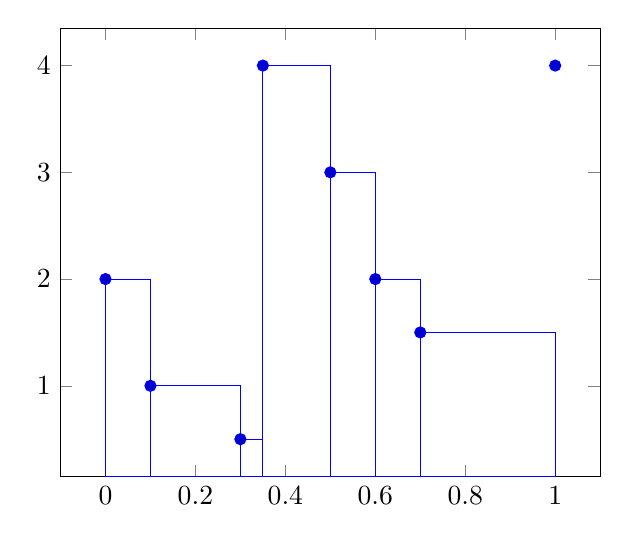
\begin{tikzpicture}
\begin{axis}
\addplot+[ybar interval] plot coordinates
	{(0,2) (0.1,1) (0.3,0.5) (0.35,4) (0.5,3)
	 (0.6,2) (0.7,1.5) (1,4)};
\end{axis}
\end{tikzpicture}
\end{codeexample}

\begin{codeexample}[]
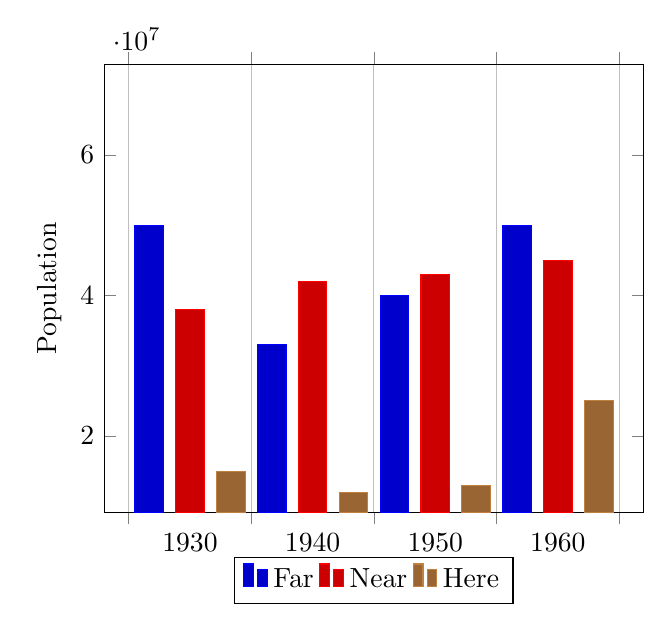
\begin{tikzpicture}
\begin{axis}[
	x tick label style={
		/pgf/number format/set thousands separator=},
	ylabel=Population,
	enlargelimits=0.05,
	legend style={at={(0.5,-0.1)},
		anchor=north,legend columns=-1},
	ybar interval=0.7,
]
\addplot[draw=blue,fill=blue!80!black] 
	coordinates {(1930,50e6) (1940,33e6)
		 (1950,40e6) (1960,50e6) (1970,70e6)};

\addplot[red,fill=red!80!black] 
	coordinates {(1930,38e6) (1940,42e6) 
		(1950,43e6) (1960,45e6) (1970,65e6)};

\addplot[brown,fill=brown!80!black] 
	coordinates {(1930,15e6) (1940,12e6) 
		(1950,13e6) (1960,25e6) (1970,35e6)};
\legend{Far,Near,Here}
\end{axis}
\end{tikzpicture}
\end{codeexample}
\end{plottype}

\begin{stylekey}{/pgfplots/ybar interval=\marg{relative width} (default 1)}
	FIXME
\end{stylekey}

\begin{plottype}{xbar interval}
\begin{codeexample}[]
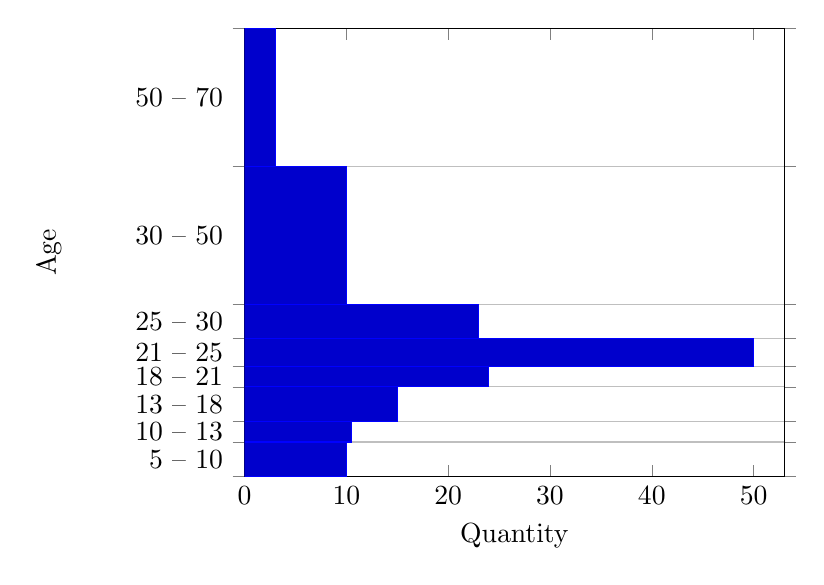
\begin{tikzpicture}
\begin{axis}[
	xmin=0,xmax=53,
	ylabel=Age,
	xlabel=Quantity,
	y label style={yshift=0.7cm},
	enlargelimits=false,
	ytick=data,
	yticklabel interval boundaries,
	xbar interval,
]
\addplot[draw=blue,mark=none,fill=blue!80!black]
	coordinates {(10,5) (10.5,10) (15,13) 
		(24,18) (50,21) (23,25) (10,30) 
		(3,50) (3,70)};
\end{axis}
\end{tikzpicture}
\end{codeexample}
\end{plottype}

\begin{stylekey}{/pgfplots/xbar interval=\marg{relative width} (default 1)}
	FIXME
\end{stylekey}

\begin{pgfplotsxykey}{\x ticklabel interval boundaries}
	These are style keys which set |x tick label as interval| and configure the tick appearance to be \marg{start} -- \marg{end} for each tick interval.

	FIXME EXAMPLE
\end{pgfplotsxykey}

\subsubsection{Comb plots}
Comb plots are very similar to bar plots except that they emplot single horizontal/vertical lines instead of rectangles.

\begin{plottype}{xcomb}
\end{plottype}

\begin{plottype}{ycomb}
\end{plottype}

\subsubsection{Stacked plots}
\begin{pgfplotskey}{stack plots=\mchoice{x,y,false} (initially false)}
FIXME
\end{pgfplotskey}

\begin{pgfplotskey}{stack dir=\mchoice{plus,minus} (initially plus)}
	FIXME
\end{pgfplotskey}

\begin{pgfplotskey}{reverse stacked plots=\mchoice{true,false} (initially true, default true)}
	FIXME
\end{pgfplotskey}

\begin{stylekey}{/pgfplots/xbar stacked=\mchoice{plus,minus} (default plus)}
	FIXME
\end{stylekey}
\begin{stylekey}{/pgfplots/ybar stacked=\mchoice{plus,minus} (default plus)}
	FIXME
\end{stylekey}

\begin{stylekey}{/pgfplots/xbar interval stacked=\mchoice{plus,minus} (default plus)}
	FIXME
\end{stylekey}
\begin{stylekey}{/pgfplots/ybar interval stacked=\mchoice{plus,minus} (default plus)}
	FIXME
\end{stylekey}

\subsubsection{Area plots}
FIXME

provide examples with |\closedcycle| and |stack plots=..|

\subsection{Markers and Linestyles}
\label{sec:markers}%
The following options of \Tikz\ are available to plots.
\subsubsection{Markers}
This list is copied from~\cite[section~29]{tikz}:
\begingroup
\newenvironment{longdescription}[0]{%
	\begin{list}{}{%
		\leftmargin=4.3cm
		\setlength{\labelwidth}{4.3cm}%
		\renewcommand{\makelabel}[1]{\hfill\textbf{\texttt{##1}}}%
	}%
}{%
	\end{list}%
}%
\def\showit#1{%
	\tikz\draw[%
		gray,
		thin,
		mark options={fill=yellow!80!black,draw=black,scale=2},
		x=0.8cm,y=0.3cm,
		#1]
	plot coordinates {(0,0) (1,1) (2,0) (3,1)};%
}%
\begin{longdescription}
	\item[mark=*] \showit{mark=*}
	\item[mark=x] \showit{mark=x}
	\item[mark=+] \showit{mark=+}
	\item[mark=ball] \showit{mark=ball}
\end{longdescription}
And with \lstinline!\usetikzlibrary{plotmarks}!:
\begin{longdescription}
	\item[mark=$-$] \showit{mark=-}
	\item[mark=$\|$] \showit{mark=|}
	\item[mark=o] \showit{mark=o}
	\item[mark=asterisk] \showit{mark=asterisk}
	\item[mark=star] \showit{mark=star}
	\item[mark=oplus] \showit{mark=oplus}
	\item[mark=oplus*] \showit{mark=oplus*}
	\item[mark=otimes] \showit{mark=otimes}
	\item[mark=otimes*] \showit{mark=otimes*}
	\item[mark=square] \showit{mark=square}
	\item[mark=square*] \showit{mark=square*}
	\item[mark=triangle] \showit{mark=triangle}
	\item[mark=triangle*] \showit{mark=triangle*}
	\item[mark=diamond] \showit{mark=diamond}
	\item[mark=diamond*] \showit{mark=diamond*}
	\item[mark=pentagon] \showit{mark=pentagon}
	\item[mark=pentagon*] \showit{mark=pentagon*}
\end{longdescription}
All these options have been drawn with the additional options
\begin{codeexample}[code only]
\draw[
	gray,
	thin,
	mark options={%
		scale=2,fill=yellow!80!black,draw=black
	}
]
\end{codeexample}

\subsubsection{Line styles}
\def\showit#1{%
	\tikz\draw[%
		black,
		x=0.8cm,y=0.3cm,
		#1]
	plot coordinates {(0,0) (1,1) (2,0) (3,1)};%
}%
The following line styles are predefined in \Tikz.
\begin{stylekey}{/tikz/solid}
	 \showit{style=solid}
\end{stylekey}

\begin{stylekey}{/tikz/dotted}
	 \showit{style=dotted}
\end{stylekey}

\begin{stylekey}{/tikz/densely dotted}
	 \showit{style=densely dotted}
\end{stylekey}

\begin{stylekey}{/tikz/loosely dotted}
	 \showit{style=loosely dotted}
\end{stylekey}

\begin{stylekey}{/tikz/dashed}
	 \showit{style=dashed}
\end{stylekey}

\begin{stylekey}{/tikz/densely dashed}
	 \showit{style=densely dashed}
\end{stylekey}

\begin{stylekey}{/tikz/loosely dashed}
	 \showit{style=loosely dashed}
\end{stylekey}
You may need the option \lstinline!mark options={solid}! to avoid dotted or dashed marker boundaries. The string ``\texttt{style=}'' can be omitted.
\endgroup

\subsubsection{Font size and line width}
Often, one wants to change line width and font sizes for plots. This can be done using the following options of \Tikz.

\begin{key}{/tikz/font=\marg{font name} (initially \textbackslash normalfont)}
	Sets the font which is to be used for text in nodes (like tick labels, legends or descriptions).
\end{key}

\begin{key}{/tikz/line width=\marg{dimension} (initially 0.4pt)}
	Sets the line width. Please note that line widths for tick lines and grid lines are predefined, so you may need to override the styles |every tick| and |every axis grid|.

	Please note that |line width| is changed quite often. You should use
\begin{codeexample}[code only]
\tikzstyle{every axis}+=[line width=1pt]
\end{codeexample}
	or
\begin{codeexample}[code only]
\tikzstyle{every axis}+=[thick]
\end{codeexample}
	to change the overall line width. To also adjust ticks and grid lines, you can use
\begin{codeexample}[code only]
\tikzstyle{every axis}+=[line width=1pt,tick style={line width=0.6pt}]
\end{codeexample}
	or styles like
\begin{codeexample}[code only]
\tikzstyle{every axis}+=[thick,tick style={semithick}]
\end{codeexample}
\end{key}

\begin{keylist}[/tikz]{ultra thin,very thin,semithick,thick,very thick,ultra thick}
	These \Tikz\ styles provide different predefined line widths.
\end{keylist}

This example shows the same plots as on page~\pageref{page:plotcoords:src}, with different line width and font size.
\begin{codeexample}[]
\tikzstyle{every axis}+=[
	font=\large,
	line width=1pt,
	tick style={line width=0.8pt}]
\begin{tikzpicture}
	\begin{loglogaxis}[
		legend style={at={(0.03,0.03)},
			anchor=south west},
		xlabel=\textsc{Dof},
		ylabel=$L_2$ Error
	]
	\plotcoords
	\legend{$d=2$,$d=3$,$d=4$,$d=5$,$d=6$}
	\end{loglogaxis}
\end{tikzpicture}
\end{codeexample}

\begin{codeexample}[]
\tikzstyle{every axis}+=[
	font=\footnotesize,
	thin,
	tick style={ultra thin}]
\begin{tikzpicture}
	\begin{loglogaxis}[
		xlabel=\textsc{Dof},
		ylabel=$L_2$ Error
	]
	\plotcoords
	\legend{$d=2$,$d=3$,$d=4$,$d=5$,$d=6$}
	\end{loglogaxis}
\end{tikzpicture}
\end{codeexample}

\subsubsection{Options controlling linestyles}

\label{sec:cycle:list}%
\begin{pgfplotskeylist}{cycle list=\marg{list},cycle list name=\marg{\textbackslash macro}}
Allows to specify a list of plot specifications which will be used for each \hbox{\lstinline!\addplot!}-command without explicit plot specification.

There are several possiblities to change it:
\begin{enumerate}
	\item Use one of the predefined lists,
\begin{codeexample}[]
\begin{tikzpicture}
\begin{loglogaxis}[
	cycle list name=\coloredplotspeclist]
\plotcoords
\legend{$d=2$,$d=3$,$d=4$,$d=5$,$d=6$}
\end{loglogaxis}
\end{tikzpicture}
\end{codeexample}
These examples employs the same coords as in the example on page~\pageref{page:plotcoords:src}.
\begin{codeexample}[]
\begin{tikzpicture}
\begin{loglogaxis}[
	cycle list name=\blackwhiteplotspeclist]
\plotcoords
\legend{$d=2$,$d=3$,$d=4$,$d=5$,$d=6$}
\end{loglogaxis}
\end{tikzpicture}
\end{codeexample}
	\item Provide the list explicitly,
\begin{codeexample}[]
\begin{tikzpicture}
\begin{loglogaxis}[cycle list={%
	{blue,mark=*},
	{red,mark=square},
	{dashed,mark=o},
	{loosely dotted,mark=+},
	{brown!60!black,
		mark options={fill=brown!40},
		mark=otimes*}}
]
\plotcoords
\legend{$d=2$,$d=3$,$d=4$,$d=5$,$d=6$}
\end{loglogaxis}
\end{tikzpicture}
\end{codeexample}
	(This example list requires \lstinline!\usetikzlibrary{plotmarks}!).
	\item Define macro names and use them with `\texttt{cycle list name}':
\begin{codeexample}[code only]
\pgfcreateplotcyclelist{\mylist}{%
	{blue,mark=*},
	{red,mark=square},
	{dashed,mark=o},
	{loosely dotted,mark=+},
	{brown!60!black,mark options={fill=brown!40},mark=otimes*}}
}
...
\begin{axis}[cycle list name=\mylist]
	...
\end{axis}
\end{codeexample}
\end{enumerate}

\paragraph{Remark:} You can also terminate single entries with `\lstinline!\\!' as in
\begin{codeexample}[code only]
\begin{axis}[cycle list={%
	blue,mark=*\\%
	red,mark=square\\%
	dashed,mark=o\\%
	loosely dotted,mark=+\\%
	brown!60!black,
		mark options={fill=brown!40},
		mark=otimes*\\}
]
...
\end{axis}
\end{codeexample}
In this case, the \emph{last} entry also needs a terminating `\lstinline!\\!', but you can omit braces around the single entries.
\end{pgfplotskeylist}




\subsection{Axis descriptions}

\begin{pgfplotsxykey}{\x label=\marg{text}}
The options \texttt{xlabel} and \texttt{ylabel} change axis labels to \marg{text} which is any \TeX\ text. Use |xlabel={text}| if you need to include `|=|' or `|,|' literally.

Labels are \Tikz-Nodes which are placed with
\begin{codeexample}[code only]
\node 
	[style=every axis label,
	style=every axis x label]
\node 
	[style=every axis label,
	style=every axis y label] 
\end{codeexample}
so their position and appearance can be customized. As for legends, the coordinate \lstinline!(0,0)! denotes the lower left axis corner and \lstinline!(1,1)! the upper right. 

The default styles are
\begin{codeexample}[code only]
\tikzstyle{every axis label}=[]
\tikzstyle{every axis x label}=[
	at={(0.5,0)},
	below,
	yshift=-15pt]
\tikzstyle{every axis y label}=[
	at={(0,0.5)},
	xshift=-35pt,
	rotate=90]
\end{codeexample}
Please only add options using |+=| instead of overwriting the default styles to ensure compatibility with future versions.
\begin{codeexample}[code only]
\tikzstyle{every axis label}+=[...]
\tikzstyle{every axis x label}+=[...]
\tikzstyle{every axis y label}+=[...]
\end{codeexample}
\end{pgfplotsxykey}

\begin{pgfplotskey}{title=\marg{text}}
Adds a caption to the plot. This will place a \Tikz-Node with
\begin{codeexample}[code only]
\node[style=every axis title] {text};
\end{codeexample}
to the current axis.
\begin{codeexample}[]
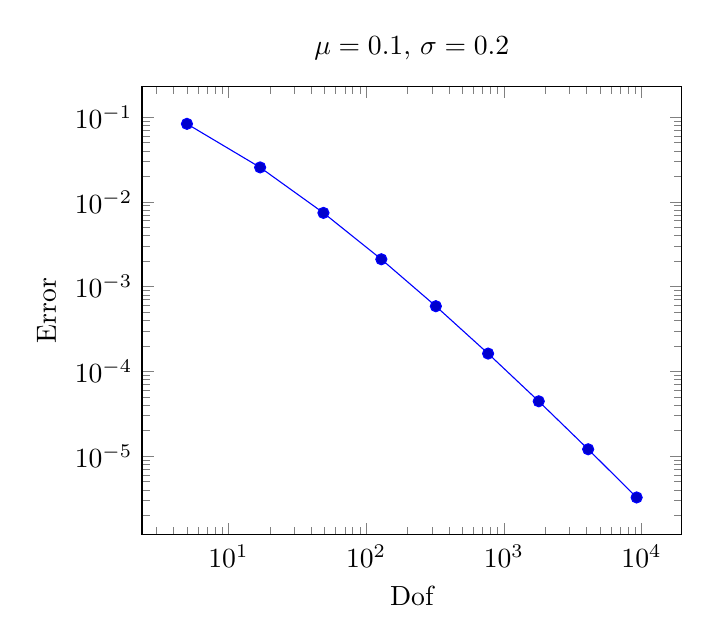
\begin{tikzpicture}
\begin{loglogaxis}[
	xlabel=Dof,ylabel=Error,
	title={$\mu=0.1$, $\sigma=0.2$}]

	\addplot coordinates {
		(5,		8.312e-02)
		(17,	2.547e-02)
		(49,	7.407e-03)
		(129,	2.102e-03)
		(321,	5.874e-04)
		(769,	1.623e-04)
		(1793,	4.442e-05)
		(4097,	1.207e-05)
		(9217,	3.261e-06)
	};
\end{loglogaxis}
\end{tikzpicture}%
\end{codeexample}
%--------------------------------------------------
% \hfill
% \begin{tikzpicture}
% \begin{loglogaxis}[
% 	width=0.48\linewidth,
% 	xlabel=Dof,ylabel=Error,
% 	title={$\mu=1$, $\sigma=\frac{1}{2}$}]
% 
% 	\addplot[color=red,mark=*] coordinates {
% 		(7,		8.472e-02)
% 		(31,	3.044e-02)
% 		(111,	1.022e-02)
% 		(351,	3.303e-03)
% 		(1023,	1.039e-03)
% 		(2815,	3.196e-04)
% 		(7423,	9.658e-05)
% 		(18943,	2.873e-05)
% 		(47103,	8.437e-06)
% 	};
% \end{loglogaxis}
% \end{tikzpicture}
%-------------------------------------------------- 
 The title is placed in the middle of the axis (the placing does not incorporate any axis descriptions). You can reconfigure the appearance and/or placing of the title for example with
\begin{codeexample}[code only]
\tikzstyle{every axis title}+=[at={(0.75,1)}]
\end{codeexample}
This will place the title at~75\% of the $x$-axis. The coordinate~$(0,0)$ is the lower left corner and~$(1,1)$ the upper right one.
\end{pgfplotskey}

\begin{pgfplotskey}{legend columns=\marg{number} (default 1)}
Allows to configure the maximum number of adjacent legend entries. The default is \texttt{legend columns=1}, so legends are placed vertically below each other. Examples can be found in section~\ref{sec:legendexamples:cols}.
\end{pgfplotskey}

\begin{pgfplotskey}{legend plot pos=\mchoice{left,right,none} (initially left)}
Configures where the small line specifications will be drawn: left of the description, right of the description or not at all. See an example in section~\ref{sec:legendexamples:plotpos}.
\end{pgfplotskey}

\begin{pgfplotscodekey}{legend image code}
\label{opt:legend:image:code}
Allows to replace the default images which are drawn inside of legends. The first argument to this option is the plot specification, a key-value list which has been determined by \lstinline!\addplot!.

The default is
\begin{codeexample}[code only]
/pgfplots/legend image code/.code={%
	\draw[#1,mark repeat=2,mark phase=2] 
		plot coordinates {
			(0cm,0cm) 
			(0.3cm,0cm)
			(0.6cm,0cm)%
		};%
}
\end{codeexample}
This default is inappropriate for bar or comb plots, see figure~\ref{fig:bar:and:comb} on page~\pageref{fig:bar:and:comb} for an example.
\end{pgfplotscodekey}

\subsection{Scaling Options}

\begin{pgfplotskey}{width=\marg{dimen}}
Sets the width of the final picture to \marg{dimen}. If no |height| is specified, scaling will respect aspect ratios.

\noindent\underline{Remarks:} 
\begin{itemize}
	\item The scaling only affects the width of one unit in $x$-direction or the height for one unit in $y$-direction. Axis labels and tick labels won't be resized, but their size is used to determine the axis scaling.

	\item You can use the \Tikz-\lstinline!scale=NUMBER! option,
	\begin{codeexample}[code only]
		\begin{tikzpicture}[scale=2]
		\begin{axis}
		...
		\end{axis}
		\end{tikzpicture}
	\end{codeexample}
	to scale the complete picture.

	\item The \Tikz-options \lstinline!x! and \lstinline!y! which set the unit dimensions in $x$ and $y$ directions can be specified as arguments to \lstinline!\begin{axis}[x=1.5cm,y=2cm]! if needed (see below). These settings override the \lstinline!width! and \lstinline!height! options.

	\item You can also force a fixed width/height of the axis (without looking at labels) with
	\begin{codeexample}[code only]
\begin{tikzpicture}
\begin{axis}[width=5cm,scale only axis]
	...
\end{axis}
\end{tikzpicture}
	\end{codeexample}

	\item Please note that up to the writing of this manual, \PGFPlots\ only estimates the size needed for axis- and tick labels. It does not include legends which have been placed outside of the axis\footnote{I.e. the `\texttt{width}' option will not work as expected, but the bounding box is still ok.}. This may be fixed in future versions.

	Use the \lstinline!x=DIMEN!, \lstinline!y=DIMEN! and \lstinline!scale only axis! options if the scaling happens to be wrong.
\end{itemize}
\end{pgfplotskey}

\begin{pgfplotskey}{height=\marg{dimen}}
	See |width|.
\end{pgfplotskey}

\begin{pgfplotskey}{scale only axis=\mchoice{true,false} (initially false)}
This boolean option allows to apply \texttt{width} and \texttt{height} only to the axis rectangle. If `\texttt{scale only axis}' is enabled, label, tick and legend dimensions won't influence the size of the axis rectangle.

If \texttt{scale only axis=false} (the default), \PGFPlots\ will try to produce the desired width \emph{including} labels, titles and ticks.
\end{pgfplotskey}

\begin{pgfplotsxykey}{\x=\marg{dimen}}
Sets the unit size for one $x$ (or $y$) coordinate to \marg{dimen}.

	Setting $x$ explicitly overrides the \lstinline!width! option. Setting $y$ explicitly overrides the \lstinline!height! option.

	Please note that it is \emph{not} possible to specify \lstinline!x! as argument to \lstinline!tikzpicture!. The option 
	\begin{codeexample}[code only]
		\begin{tikzpicture}[x=1.5cm]
		\begin{axis}
			...
		\end{axis}
		\end{tikzpicture}
	\end{codeexample}
	won't have any effect because an axis rescales its coordinates (see the \lstinline!width! option).
\end{pgfplotsxykey}

\subsection{Error bars}
\label{sec:errorbars}
{%
\def\pgfplotserror#1{\ensuremath{\epsilon_{#1}}}%
\PGFPlots\ supports error bars for normal and logarithmic plots. 

Error bars are enabled for each plot separately, using \meta{behavior options} after \lstinline!\addplot!:
\begin{codeexample}[code only]
\addplot plot[/pgfplots/error bars/.cd,x dir=both,y dir=both] ...
\end{codeexample}
Error bars inherit all drawing options of the associated plot, but they use their own marker and style arguments additionally.

\begin{codeexample}[]
\begin{tikzpicture}
\begin{axis}
\addplot plot[/pgfplots/error bars/.cd,
	y dir=plus,y explicit]
coordinates {(0,0) +- (0.5,0.1) 
	(0.1,0.1)  +- (0.05,0.2)
	(0.2,0.2) 	+- (0,0.05)
	(0.5,0.5) +- (0.1,0.2)
	(1,1) +- (0.3,0.1)};
\end{axis}
\end{tikzpicture}
\end{codeexample}

\begin{codeexample}[]
\begin{tikzpicture}
\begin{axis}
\addplot plot[/pgfplots/error bars/.cd,
	y dir=both,y explicit,
	x dir=both,x fixed=0.05,
	error mark=diamond*]
coordinates {(0,0) +- (0.5,0.1) 
	(0.1,0.1)  +- (0.05,0.2)
	(0.2,0.2) 	+- (0,0.05)
	(0.5,0.5) +- (0.1,0.2)
	(1,1) +- (0.3,0.1)};
\end{axis}
\end{tikzpicture}
\end{codeexample}

\begin{codeexample}[]
\begin{tikzpicture}
\begin{loglogaxis}
\addplot plot[/pgfplots/error bars/.cd,
	x dir=both,x fixed relative=0.5,
	y dir=both,y explicit relative,
	error mark=triangle*]
coordinates {
	(32,32)
	(64,64)
	(128,128) +- (0,0.3)
	(1024,1024) +- (0,0.2)
	(32068,32068)  +- (0,0.6)
	(64000,64000) +- (0,0.6)
	(128000,128000) +- (0,0.6)
};
%--------------------------------------------------
% table[x=XCol,y=YCol,
% 	x error=XErrCol,y error=YErrCol]
% 	{<file>};
%-------------------------------------------------- 
\end{loglogaxis}
\end{tikzpicture}
\end{codeexample}

\begin{codeexample}[]
\begin{tikzpicture}
\begin{axis}[enlargelimits=false]
\addplot[red,mark=*] 
	plot[/pgfplots/error bars/.cd,
	y dir=minus,y fixed relative=1,
	x dir=minus,x fixed relative=1,
	error mark=none,
	error bar style={dotted}]
coordinates
	{(0,0) (0.1,0.1)  (0.2,0.2) 	
	(0.5,0.5) (1,1)};
\end{axis}
\end{tikzpicture}
\end{codeexample}

\begin{pgfplotsxykey}{error bars/\x\ dir=\mchoice{none,plus,minus,both} (initially none)}
Draws either no error bars at all, only marks at $x+\pgfplotserror x$, only marks at $x-\pgfplotserror x$ or marks at both, $x+\pgfplotserror x$ and $x-\pgfplotserror x$. The $x$-error $\pgfplotserror x$ is acquired using one of the following options.

The same holds for the |y dir| option.
\end{pgfplotsxykey}

\begin{pgfplotsxykey}{error bars/\x\ fixed=\marg{value} (initially 0)}
Provides a common, absolute error $\pgfplotserror x=\text{\texttt{VAL}}$ for all input coordinates.

For linear $x$~axes, the error mark is drawn at $x \pm \pgfplotserror x$ while for logarithmic $x$~axes, it is drawn at $\log( x \pm \pgfplotserror x)$. Computations are performed in \PGF's floating point arithmetics.
\end{pgfplotsxykey}

\begin{pgfplotsxykey}{error bars/\x\ fixed relative=\marg{percent} (initially 0)}
Provides a common, relative error $\pgfplotserror x = \text{\texttt{VAL}} \cdot x$ for all input coordinates. \texttt{VAL} is thus given relatively to input $x$ coordinates such that $\text{\texttt{VAL}} = 1$ means $100\%$.

Error marks are thus placed at $x \cdot (1 \pm \pgfplotserror x)$ for linear axes and at $\log(x \cdot (1 \pm \pgfplotserror x))$ for logarithmic axes. Computations are performed in floating point for linear axis and using the identity $\log(x \cdot (1 \pm \pgfplotserror x)) = \log(x) + \log( 1 \pm \pgfplotserror x)$ for logarithmic scales.
\end{pgfplotsxykey}

\begin{pgfplotsxykey}{error bars/\x\ explicit}
Configures the error bar algorithm to draw $x$-error bars at any input coordinate for which user-specified errors are available.
 Each error is interpreted as absolute error, see \texttt{x fixed} for details.

The different input formats of errors are described in section~\ref{sec:errorbar:input}.
\end{pgfplotsxykey}

\begin{pgfplotsxykey}{error bars/\x\ explicit relative}
Configures the error bar algorithm to draw $x$-error bars at any input coordinate for which user-specified errors are available.
 Each error is interpreted as relative error, that means error marks are placed at $x (1 \pm \text{\texttt{VAL}})$ (works as for \texttt{error bars/x fixed relative}).
\end{pgfplotsxykey}


\begin{pgfplotskey}{error bars/error mark=\meta{marker}}
Sets an error marker for any error bar. \texttt{MARKER} is expected to be a valid plot mark, see section~\ref{sec:markers}.
\end{pgfplotskey}

\begin{pgfplotskey}{error bars/error mark options=\marg{key-value-list}}
Sets a key-value list of options for any error mark. This option works similary to the \Tikz\ `\texttt{mark options}' key.
\end{pgfplotskey}

\begin{pgfplotskey}{error bars/error bar style=\marg{key-value-list}}
Appends the argument to `\texttt{/tikz/every error bar}' which is installed at the beginning of every error bar.
\end{pgfplotskey}

\begin{pgfplotscodetwokey}{error bars/draw error bar}
Allows to change the default drawing commands for error bars. The two arguments are
\begin{itemize} 
\item the source point, $(x,y)$ and
\item the target point, $(\tilde x,\tilde y)$.
\end{itemize}
Both are determined by \PGFPlots\ according to the options described above. The default code is
\begin{codeexample}[code only][basicstyle=\footnotesize\ttfamily]
/pgfplots/error bars/draw error bar/.code 2 args={%
	\pgfkeysgetvalue{/pgfplots/error bars/error mark}%
		{\pgfplotserrorbarsmark}%
	\pgfkeysgetvalue{/pgfplots/error bars/error mark options}%
		{\pgfplotserrorbarsmarkopts}%
	\draw #1 -- #2 node[pos=1,sloped,allow upside down] {%
		\expandafter\tikz\expandafter[\pgfplotserrorbarsmarkopts]{%
			\expandafter\pgfuseplotmark\expandafter{\pgfplotserrorbarsmark}%
			\pgfusepath{stroke}}%
	};
}
\end{codeexample}
\end{pgfplotscodetwokey}

\subsubsection{Input formats of error coordinates}
\label{sec:errorbar:input}%
Error bars with explicit error estimations for single data points require some sort of input format. This applies to `\texttt{error bars/[xy] explizit}' and `\texttt{error bars/[xy] explizit relative}'.

Error bar coordinates can be read from `\texttt{plot coordinates}' or from `\texttt{plot table}'. The inline plot coordinates format is
\begin{codeexample}[code only]
\addplot coordinates {
	(1,2) +- (0.4,0.2)
	(2,4) +- (1,0)
	(3,5)
	(4,6) +- (0.3,0.001)
}
\end{codeexample}
where $(1,2) \pm (0.4,0.2)$ is the first coordinate, $(2,4) \pm (1,0)$ the second and so forth. The point $(3,5)$ has no error coordinate.

The `\texttt{plot table}' format is
\begin{codeexample}[code only]
\addplot table[x error=COLNAME,y error=COLNAME]
\end{codeexample}
or
\begin{codeexample}[code only]
\addplot table[x error index=COLINDEX,y error index=COLINDEX]
\end{codeexample}
These options are used as the `\texttt{x}' and `\texttt{x index}' options.

You can supply error coordinates even if they are not used at all; they will be ignored silently in this case.

}%

\subsection{Number formatting options}
{
\pgfkeys{/codeexample/every code example/.append style={width=4cm}}
\begin{command}{\pgfmathprintnumber{\marg{x}}}
Generates pretty-printed output for the (real) number \marg{x}. The input number \marg{x} is parsed using |\pgfmathfloatparsenumber| which allows arbitrary precision.

Numbers are typeset in math mode using the current set of number printing options, see below.
\end{command}

\begin{key}{/pgf/number format/fixed}
Configures |\pgfmathprintnumber| to round the number to a fixed number of digits after the period, discarding any trailing zeros.

\begin{codeexample}[]
\pgfkeys{/pgf/number format/.cd,fixed,precision=2}
\pgfmathprintnumber{4.568}\hspace{1em}
\pgfmathprintnumber{5e-04}\hspace{1em}
\pgfmathprintnumber{0.1}\hspace{1em}
\pgfmathprintnumber{24415.98123}\hspace{1em}
\pgfmathprintnumber{123456.12345}
\end{codeexample}

See section~\ref{sec:number:styles} for how to change the appearance.
\end{key}

\begin{key}{/pgf/number format/fixed zerofill}
Configures |\pgfmathprintnumber| to round the number to a fixed number of digits after the period, filling missing digits after the period with zeros.

\begin{codeexample}[]
\pgfkeys{/pgf/number format/.cd,fixed zerofill,precision=2}
\pgfmathprintnumber{4.568}\hspace{1em}
\pgfmathprintnumber{5e-04}\hspace{1em}
\pgfmathprintnumber{0.1}\hspace{1em}
\pgfmathprintnumber{24415.98123}\hspace{1em}
\pgfmathprintnumber{123456.12345}
\end{codeexample}

See section~\ref{sec:number:styles} for how to change the appearance.
\end{key}

\begin{key}{/pgf/number format/sci}
Configures |\pgfmathprintnumber| to display numbers in scientific format, that means sign, mantisse and exponent (basis~$10$). The mantisse is rounded to the desired precision.

\begin{codeexample}[]
\pgfkeys{/pgf/number format/.cd,sci,precision=2}
\pgfmathprintnumber{4.568}\hspace{1em}
\pgfmathprintnumber{5e-04}\hspace{1em}
\pgfmathprintnumber{0.1}\hspace{1em}
\pgfmathprintnumber{24415.98123}\hspace{1em}
\pgfmathprintnumber{123456.12345}
\end{codeexample}

See section~\ref{sec:number:styles} for how to change the exponential display style.
\end{key}

\begin{key}{/pgf/number format/sci zerofill}
As above, but the mantisse is rounded using `\texttt{fixed zerofill}'.

\begin{codeexample}[]
\pgfkeys{/pgf/number format/.cd,sci zerofill,precision=2}
\pgfmathprintnumber{4.568}\hspace{1em}
\pgfmathprintnumber{5e-04}\hspace{1em}
\pgfmathprintnumber{0.1}\hspace{1em}
\pgfmathprintnumber{24415.98123}\hspace{1em}
\pgfmathprintnumber{123456.12345}
\end{codeexample}

See section~\ref{sec:number:styles} for how to change the exponential display style.
\end{key}


\begin{key}{/pgf/number format/std}
Configures |\pgfmathprintnumber| to a standard algorithm. It chooses either \texttt{fixed} or \texttt{sci}, depending on the order of magnitude. Let $n=s \cdot m \cdot 10^e$ be the input number and $p$ the current precision. If $-p/2 \le e \le 4$, the number is displayed using the fixed format. Otherwise, it is displayed using the scientific format. 

\begin{codeexample}[]
\pgfkeys{/pgf/number format/.cd,std,precision=2}
\pgfmathprintnumber{4.568}\hspace{1em}
\pgfmathprintnumber{5e-04}\hspace{1em}
\pgfmathprintnumber{0.1}\hspace{1em}
\pgfmathprintnumber{24415.98123}\hspace{1em}
\pgfmathprintnumber{123456.12345}
\end{codeexample}
\end{key}

\begin{key}{/pgf/number format/int detect}
Configures |\pgfmathprintnumber| to detect integers automatically. If the input number is an integer, no period is displayed at all. If not, the scientific format is choosen.

\begin{codeexample}[]
\pgfkeys{/pgf/number format/.cd,int detect,precision=2}
\pgfmathprintnumber{15}\hspace{1em}
\pgfmathprintnumber{20}\hspace{1em}
\pgfmathprintnumber{20.4}\hspace{1em}
\pgfmathprintnumber{0.01}\hspace{1em}
\pgfmathprintnumber{0}
\end{codeexample}
\end{key}

\begin{key}{/pgf/number format/int trunc}
Truncates every number to integers (discards any digit after the period).

\begin{codeexample}[]
\pgfkeys{/pgf/number format/.cd,int trunc}
\pgfmathprintnumber{4.568}\hspace{1em}
\pgfmathprintnumber{5e-04}\hspace{1em}
\pgfmathprintnumber{0.1}\hspace{1em}
\pgfmathprintnumber{24415.98123}\hspace{1em}
\pgfmathprintnumber{123456.12345}
\end{codeexample}
\end{key}

\begin{key}{/pgf/number format/precision=\marg{number}}
Sets the desired rounding precision for any display operation. For scientific format, this affects the mantisse.
\end{key}

\subsubsection{Changing display styles}%
\label{sec:number:styles}%
You can change the way how numbers are displayed. For example, if you use the `\texttt{fixed}' style, the input number is rounded to the desired precision and the current fixed point display style is used to typeset the number. The same is applied to any other format: first, rounding routines are used to get the correct digits, afterwards a display style generates proper \TeX-code.

\begin{key}{/pgf/number format/set decimal separator=\marg{text}}
Assigns \marg{text} as decimal separator for any fixed point numbers (including the mantisse in sci format).
\end{key}

\begin{key}{/pgf/number format/set thousands separator=\marg{text}}
Assigns \marg{text} as thousands separator for any fixed point numbers (including the mantisse in sci format).

\begin{codeexample}[]
\pgfkeys{/pgf/number format/.cd,
	fixed zerofill,
	precision=2,
	set thousands separator={}}
\pgfmathprintnumber{1234.56}
\end{codeexample}
\begin{codeexample}[]
\pgfkeys{/pgf/number format/.cd,
	fixed zerofill,
	precision=2,
	set thousands separator={}}
\pgfmathprintnumber{1234567890}
\end{codeexample}

\begin{codeexample}[]
\pgfkeys{/pgf/number format/.cd,
	fixed zerofill,
	precision=2,
	set thousands separator={.}}
\pgfmathprintnumber{1234567890}
\end{codeexample}
\begin{codeexample}[]
\pgfkeys{/pgf/number format/.cd,
	fixed zerofill,
	precision=2,
	set thousands separator={,}}
\pgfmathprintnumber{1234567890}
\end{codeexample}
\begin{codeexample}[]
\pgfkeys{/pgf/number format/.cd,
	fixed zerofill,
	precision=2,
	set thousands separator={\relax{,}}}
\pgfmathprintnumber{1234567890}
\end{codeexample}
The last example employs commas and disables the default comma-spacing. The \texttt{\textbackslash relax} command is a technical thing which enables \pgfname keys to recognize the braces.
\end{key}

\begin{key}{/pgf/number format/use period}
A predefined style which installs periods `\texttt{.}' as decimal separators and commas `\texttt{,}' as thousands separators. This style is the default.

\begin{codeexample}[]
\pgfkeys{/pgf/number format/.cd,fixed,precision=2,use period}
\pgfmathprintnumber{12.3456}
\end{codeexample}
\begin{codeexample}[]
\pgfkeys{/pgf/number format/.cd,fixed,precision=2,use period}
\pgfmathprintnumber{1234.56}
\end{codeexample}
\end{key}

\begin{key}{/pgf/number format/use comma}
A predefined style which installs commas `\texttt{,}' as decimal separators and periods `\texttt{.}' as thousands separators.

\begin{codeexample}[]
\pgfkeys{/pgf/number format/.cd,fixed,precision=2,use comma}
\pgfmathprintnumber{12.3456}
\end{codeexample}
\begin{codeexample}[]
\pgfkeys{/pgf/number format/.cd,fixed,precision=2,use comma}
\pgfmathprintnumber{1234.56}
\end{codeexample}
\end{key}

\begin{key}{/pgf/number format/skip 0.=\marg{boolean}}
	Configures whether numbers like $0.1$ shall be typeset as $.1$ or not.
\begin{codeexample}[]
\pgfkeys{/pgf/number format/.cd,fixed zerofill,precision=2,
	skip 0.}
\pgfmathprintnumber{0.56}
\end{codeexample}
\begin{codeexample}[]
\pgfkeys{/pgf/number format/.cd,fixed zerofill,precision=2,
	skip 0.=false}
\pgfmathprintnumber{0.56}
\end{codeexample}
\end{key}

\begin{key}{/pgf/number format/sci 10e}
Uses $m \cdot 10^e$ for any number displayed in scientific format.

\begin{codeexample}[]
\pgfkeys{/pgf/number format/.cd,sci,sci 10e}
\pgfmathprintnumber{12.345}
\end{codeexample}
\end{key}

\begin{key}{/pgf/number format/sci 10\textasciicircum e}
The same as `|sci 10e|'.
\end{key}

\begin{key}{/pgf/number format/sci e}
Uses the `$1e{+}0$' format which is generated by common scientific tools for any number displayed in scientific format.

\begin{codeexample}[]
\pgfkeys{/pgf/number format/.cd,sci,sci e}
\pgfmathprintnumber{12.345}
\end{codeexample}
\end{key}

\begin{key}{/pgf/number format/sci E}
The same with an uppercase `\texttt{E}'.

\begin{codeexample}[]
\pgfkeys{/pgf/number format/.cd,sci,sci E}
\pgfmathprintnumber{12.345}
\end{codeexample}
\end{key}

\begin{key}{/pgf/number format/sci subscript}
Typesets the exponent as subscript for any number displayed in scientific format. This style requires very few space.

\begin{codeexample}[]
\pgfkeys{/pgf/number format/.cd,sci,sci subscript}
\pgfmathprintnumber{12.345}
\end{codeexample}
\end{key}
}


\label{sec:identify:minor:log}%
\begin{pgfplotskey}{log identify minor tick positions=\mchoice{true,false} (initially true)}
Set this to \texttt{true} if you want to identify log--plot tick labels at positions 
\[ i \cdot 10^j \]
with $i \in \{2,3,4,5,6,7,8,9\},\, j \in \Z$. This may be valueable in conjunction with the `\texttt{extra x ticks}' and `\texttt{extra y ticks}' options. An example is shown below: The axis range is so small that only one tick label $10^j$ is inside of it. Extra tick labels can be placed on top of the normal ticks, and placing ticks at $i \cdot 10^j $ may be appropriate.
\begin{codeexample}[]
\tikzstyle{every axis}+=[%
	width=6cm,
	xmin=7e-3,xmax=7e-2,
	extra x ticks={3e-2,6e-2},
	extra x tick style={major tick length=0pt,font=\footnotesize}
]%
\begin{tikzpicture}%
	\begin{loglogaxis}[
		title=with minor tick identification]
	\addplot coordinates {
		(1e-2,10)
		(3e-2,100)
		(6e-2,200)
	};
	\end{loglogaxis}
\end{tikzpicture}%
\hspace{0.2cm}
\begin{tikzpicture}%
	\begin{loglogaxis}[
		title=without minor tick identification,
		log identify minor tick positions=false]
	\addplot coordinates {
		(1e-2,10)
		(3e-2,100)
		(6e-2,200)
	};
	\end{loglogaxis}%
\end{tikzpicture}%
\end{codeexample}
\end{pgfplotskey}

\begin{pgfplotscodekey}{log number format code}
Provides \TeX-code to generate log plot tick labels. Argument `\texttt{\#1}' is the (natural) logarithm of the tick position.
The default implementation changes the log basis to~$10$ and invokes `\texttt{log base 10 number format code}' with the result. It also checks the other log plot options.
\end{pgfplotscodekey}


\begin{pgfplotscodekey}{log base 10 number format code}
Allows to change the overall appearance of base 10 log plot tick labels. The default is
\begin{codeexample}[code only]
log base 10 number format code/.code={%
	$10^{\pgfmathprintnumber{#1}}$}
\end{codeexample}
where the `\texttt{log plot exponent style}' allows to change number formatting options.
\end{pgfplotscodekey}

\begin{pgfplotskey}{log plot exponent style=\marg{key-value-list}}
Allows to configure the number format of log plot exponents. This style is installed just before `\texttt{log base 10 number format code}' will be invoked. Please note that this style will be installed within the default code for `\texttt{log number format code}'. Figure~\ref{fig:log:exponent:style} shows two examples.
\begin{codeexample}[]
\tikzset{samples=15}%
\tikzstyle{every axis}+=[
		width=7cm,
		xlabel=$x$,
		ylabel=$f(x)$,
		extra y ticks={45},
		legend style={at={(0.03,0.97)},anchor=north west}]%
\begin{tikzpicture}%
	\begin{semilogyaxis}[
		log plot exponent style/.style={/pgf/number format/fixed zerofill,/pgf/number format/precision=1}
	]
		\addplot plot[id=gnuplot_exp,domain=-5:10] function{exp(x)};
		\addplot plot[id=gnuplot_expv,domain=-5:10] function{exp(2*x)};
		\legend{$e^x$,$e^{2x}$}
	\end{semilogyaxis}
\end{tikzpicture}%
\end{codeexample}

\begin{codeexample}[]
\tikzset{samples=15}%
\tikzstyle{every axis}+=[
		width=7cm,
		xlabel=$x$,
		ylabel=$f(x)$,
		extra y ticks={45},
		legend style={at={(0.03,0.97)},anchor=north west}]%
\begin{tikzpicture}%
	\begin{semilogyaxis}[
		log plot exponent style/.style={/pgf/number format/fixed,/pgf/number format/use comma,/pgf/number format/precision=2}
	]
		\addplot plot[id=gnuplot_exp,domain=-5:10] function{exp(x)};
		\addplot plot[id=gnuplot_expv,domain=-5:10] function{exp(2*x)};
		\legend{$e^x$,$e^{2x}$}
	\end{semilogyaxis}
\end{tikzpicture}%
\end{codeexample}
\end{pgfplotskey}

%--------------------------------------------------
% \subsubsection{Defining own display styles}
% You can define own display styles, although this may require some insight into \TeX-programming. Here are two examples:
% \begin{enumerate}
% 	\item A new fixed point display style: The following code defines a new style named `\texttt{my own fixed point style}' which uses $1{\cdot}00$ instead of $1.00$.
% \begin{lstlisting}
% \def\myfixedpointstyleimpl#1.#2\relax{%
% 	#1{\cdot}#2%
% }%
% \def\myfixedpointstyle#1{%
% 	\pgfutilensuremath{%
% 	\ifpgfmathfloatroundhasperiod
% 		\expandafter\myfixedpointstyleimpl#1\relax
% 	\else
% 		#1%
% 	\fi
% 	}%
% }
% \pgfkeys{/my own fixed point style/.code={%
% 	\let\pgfmathprintnumber@fixed@style=\myfixedpointstyle}
% }%
% \end{codeexample}
% 	You only need to overwrite the macro \lstinline!\pgfmathprintnumber@fixed@style!. This macro takes one argument (the result of any numerical computations). The \TeX-boolean \lstinline!\ifpgfmathfloatroundhasperiod! is true if and only if the input number contains a period.
% 
% 	\item An example for a new scientific display style:
% \begin{lstlisting}
% % #1:
% % 		0 == '0' (the number is +- 0.0),
% % 		1 == '+', 
% % 		2 == '-',
% % 		3 == 'not a number'
% % 		4 == '+ infinity'
% % 		5 == '- infinity'
% % #2: the mantisse
% % #3: the exponent
% \def\myscistyle#1#2e#3\relax{%
% 	...
% }
% \pgfkeys{/my own sci style/.code={%
% 	\let\pgfmathfloatrounddisplaystyle=\myscistyle},
% }%
% \end{codeexample}
% \end{enumerate}
%-------------------------------------------------- 




\subsection{Specifying the plotted range}

\begin{pgfplotsxykeylist}{\x min=\marg{coord},\x max=\marg{coord}}
The options \texttt{xmin}, \texttt{xmax} and \texttt{ymin}, \texttt{ymax} allow to define the axis limits, i.e. the lower left and the upper right corner. Some remarks:
\begin{itemize}
	\item The axis limits determine the plotted range. Everything else will be clipped away.
	\item If one of \lstinline!xmin! or \lstinline!xmax! is missing, the $x$-interval will be determined automatically (see \lstinline!\addplot!). The same holds true if one of \lstinline!ymin! or \lstinline!ymax! is missing: in this case, the $y$-interval will be determined automatically.

	If $x$-limits have been specified explicitly and $y$-limits are computed automatically, the automatic computation of $y$-limits will only considers points which fall into the specified $x$-range (and vice--versa). See option \texttt{clip limits} for details.

	\item The option \lstinline!enlargelimits! will automatically increase the plotted range.
\end{itemize}
\end{pgfplotsxykeylist}

\begin{pgfplotsxykey}{\x mode=\mchoice{normal,linear,log} (initially normal)}
Allows to choose between linear (=normal) or logarithmic axis scaling or logplots for each $x,y$-combination.
\end{pgfplotsxykey}

\begin{pgfplotskey}{clip limits=\mchoice{true,false} (initially true)}
	Configures what to do if some, but not all axis limits have been specified explicitly. In case |clip limits=true|, the automatic limit computation will \emph{only} consider points which do not contradict the explicitly set limits. 
\end{pgfplotskey}

\begin{pgfplotskey}{enlargelimits=\mchoice{true,false,auto,\marg{val}}}
Enlarges the axis size somewhat if enabled.

You can set \texttt{xmin}, \texttt{xmax} and \texttt{ymin}, \texttt{ymax} to the minimum/maximum values of your data and \texttt{enlargelimits} will enlarge the canvas such that the axis doesn't touch the plots.

\begin{itemize}
	\item The value \texttt{true} enlarges all axes.
	\item The value \texttt{false} uses tight axis limits as specified by the user (or read from input coordinates).
	\item The value \texttt{auto} will enlarge limits only for axis for which axis limits have been determined automatically.
	\item All other values like `\texttt{enlargelimits=0.1}' will enlarge all axis limits relatively (in this example, 10\% of the axis limits will be added at all sides).
\end{itemize}
A small value of \texttt{enlargelimits} may avoid problems with large markers near the boundary.
\end{pgfplotskey}


\subsection{Tick and Grid Options}

\begin{pgfplotsxykey}{\x tick=\mchoice{\textbackslash empty,data,\marg{coordinate list}} (initially \marg{})}
The options \texttt{xtick} and \texttt{ytick} assigns a list of \emph{Positions} where ticks shall be placed. The argument is either the command |\empty|, |data| or a list of coordinates. The choice |\empty| will result in no tick at all. The special value |data| will produce tick marks at every coordinate of the first plot. Otherwise, tick marks will be placed at every coordinate in  \marg{coordinate list}. If this list is empty, \PGFPlots\ will compute a default list. 

\marg{coordinate list} will be used inside of a \lstinline!\foreach \x in !\marg{coordinate list} statement. The format is as follows:
\begin{itemize}
	\item \lstinline!{0,1,2,5,8,1e1,1.5e1}! (a series of coordinates),
	\item \lstinline!{0,...,5}! (the same as \lstinline!{0,1,2,3,4,5}!),
	\item \lstinline!{0,2,...,10}! (the same as \lstinline!{0,2,4,6,8,10}!),
	\item \lstinline!{9,...,3.5}! (the same as \lstinline!{9, 8, 7, 6, 5, 4}!),
	\item See \cite[Section~34]{tikz} for a more detailed definition of the options.
\end{itemize}
For logplots, \PGFPlots\ will apply $\log(\cdot)$ to each element in `\marg{coordinate list}'. 
\begin{codeexample}[]
\begin{tikzpicture}
	\begin{loglogaxis}[xtick={12,9897,1468864}]
	\plotcoords
	\end{loglogaxis}
\end{tikzpicture}
\end{codeexample}

\begin{codeexample}[]
\begin{tikzpicture}
\begin{axis}[
	xtick=\empty,
	ytick={-2,0.3,3,3.7,4.5}]
\addplot+[smooth] coordinates {
	(-2,3) (-1.5,2) (-0.3,-0.2) 
	(1,1.2) (2,2) (3,5)};
\end{axis}
\end{tikzpicture}
\end{codeexample}

\paragraph{Attention:} You can't use the `\texttt{...}' syntax if the elements are too large for \TeX! For example, `\texttt{xtick=1.5e5,2e7,3e8}' will work (because the elements are interpreted as strings, not as numbers), but `\texttt{xtick=1.5,3e5,...,1e10}' will fail because it involves real number arithmetics beyond \TeX's capacities.
\vspace*{0.3cm}

\noindent
The default choice for tick \emph{positions} in normal plots is to place a tick at each coordinate~$i\cdot h$. The step size~$h$ depends on the axis scaling and the axis limits. It is chosen from a list a ``feasable'' step sizes such that neither too much nor too few ticks will be generated. The default for logplots it to place ticks at positions $10^i$ in the axis' range. Which positions depends on the axis scaling and the dimensions of the picture. The default tick positions can be reconfigured with
\begin{itemize}
	\item `\lstinline!max space between ticks=!\marg{number}' where the integer argument denotes the maximum space between adjacent ticks in full points. The suffix ``\texttt{pt}'' has to be omitted and fractional numbers are not supported. The default is~\axisdefaulttickwidth.
	\item `\lstinline!try min ticks=!\marg{number}' configures a loose lower bound on the number of ticks. It should be considered as a suggestion, not a tight limit. The default is~\axisdefaulttryminticks. This number will increase the number of ticks if `\texttt{max space between ticks}' produces too few of them.
	\item `\lstinline!try min ticks log=!\marg{number}' The same for logarithmic axis.
\end{itemize}
The total number of ticks may still vary because not all fractional numbers in the axis' range are valid tick positions.


\noindent
The tick \emph{appearance} can be (re-)configured with
\begin{codeexample}[code only]
\tikzstyle{every tick}=[very thin,gray]
\tikzstyle{every minor tick}=[]
\end{codeexample}
or
\begin{codeexample}[code only]
\tikzstyle{every tick}+=[very thin,gray]
\tikzstyle{every minor tick}+=[black]
\end{codeexample}
Please prefer the `\texttt{+=}' versions to ensure compatibility with future versions.

This style commands can be used at any time. The tick line width can be configured with `\texttt{major tick length}' and `\texttt{minor tick length}'.
\end{pgfplotsxykey}

\begin{pgfplotsxykey}{extra \x\ ticks=\marg{coordinate list}}
Adds \emph{additional} tick positions and tick labels to the $x$~or~$y$ axis. `Additional' tick positions do not affect the normal tick placement algorithms, they are drawn after the normal ticks. This has two benefits: first, you can add single, important tick positions without disabling the default tick label generation and second, you can draw tick labels `on top' of others, possibly using different style flags.


\begin{codeexample}[]
\begin{tikzpicture}
\begin{axis}[
	xmin=0,xmax=3,ymin=0,ymax=15,
	extra y ticks={2.71828},
	extra y tick labels={$e$},
	extra x ticks={2.2},
	extra x tick style={grid=major,
		/pgfplots/tick label style={
			rotate=90,anchor=east}},
	extra x tick labels={Cut},
]
	\addplot (\x,{exp(\x)});
	\addlegendentry{$e^x$}
\end{axis}
\end{tikzpicture}
\end{codeexample}
\begin{codeexample}[]
\begin{tikzpicture}
\begin{loglogaxis}[width=5.5cm]
\addplot coordinates 
	{(10,1e-5) (20,5e-6) (40,2.5e-6)};
\end{loglogaxis}
\end{tikzpicture}

\begin{tikzpicture}
\begin{loglogaxis}[
	width=5.5cm,
	extra x ticks={20,40},
	extra y ticks={5e-6,2.5e-6}]
\addplot coordinates 
	{(10,1e-5) (20,5e-6) (40,2.5e-6)};
\end{loglogaxis}
\end{tikzpicture}

\begin{tikzpicture}
\begin{loglogaxis}[
	width=5.5cm,
	log identify minor tick positions=false,
	extra x ticks={20,40},
	extra y ticks={5e-6,2.5e-6}]
\addplot coordinates 
	{(10,1e-5) (20,5e-6) (40,2.5e-6)};
\end{loglogaxis}
\end{tikzpicture}
\end{codeexample}

Remarks:
\begin{itemize} 
\item Use \texttt{extra x ticks} to highlight special tick positions. The use of \texttt{extra x ticks} does not affect minor tick/grid line generation, so you can place extra ticks at positions $j\cdot 10^i$ in log--plots. 
\item Extra ticks are always typeset as major ticks, that means they employ the options `\texttt{major tick length}' and respect options like `\texttt{grid=major}'.
\item Use the style `\texttt{every extra x tick}' (`\texttt{every extra y tick}') to configure the appearance.
\item You can also use `\texttt{extra x tick style=\{...\}}' which has the same effect.
\end{itemize}
\end{pgfplotsxykey}

\begin{pgfplotskey}{space between ticks=\marg{number}}
see Options \texttt{xtick} and \texttt{ytick} for a description.
\end{pgfplotskey}

\begin{pgfplotskey}{try min ticks=\marg{number}}
see Options \texttt{xtick} and \texttt{ytick} for a description.
\end{pgfplotskey}

\begin{pgfplotskey}{try min ticks log=\marg{number}}
see Options \texttt{xtick} and \texttt{ytick} for a description.
\end{pgfplotskey}

\begin{pgfplotskeylist}{tickwidth=\marg{dimension},major tick length=\marg{dimension} (initially 0.15cm)}
	Sets the width of major tick lines.
\end{pgfplotskeylist}

\begin{pgfplotskeylist}{subtickwidth=\marg{dimension},minor tick length=\marg{dimension} (initially 0.1cm)}
	Sets the width of minor tick lines.
\end{pgfplotskeylist}

\begin{pgfplotsxykey}{\x tickten=\marg{exponent base 10 list}}
The options \texttt{xtickten} and \texttt{ytickten} allow to place ticks at selected positions $10^k, k \in \text{\marg{exponent base 10 list}}$. They are only used for logplots. The syntax for \marg{exponent base 10 list} is the same as above for |xtick=|\marg{list} or |ytick=|\marg{list}.

Using `\texttt{xtickten=\{1,2,3,4\}}' is equivalent to `\texttt{xtick=\{1e1,1e2,1e3,1e4\}}', but it requires fewer computational time and it allows to use the short syntax `\texttt{xtickten=\{1,...,4\}}'.
\begin{codeexample}[]
\begin{tikzpicture}[samples=8]
\begin{semilogyaxis}[
	ytickten={-6,-4,...,4},
	domain=0:10]

% invoke gnuplot to generate coordinates:
\addplot plot[id=pow1] function {2**(-2*x + 6)};
\addlegendentry{$2^{-2x + 6}$}

\addplot plot[id=pow2] function {2**(-1.5*x -3)};
\addlegendentry{$2^{-1.5x -3}$}
\end{semilogyaxis}
\end{tikzpicture}
\end{codeexample}
\end{pgfplotsxykey}

\begin{pgfplotsxykey}{\x ticklabels=\marg{label list}}
Assigns a \emph{list} of tick \emph{labels} to each tick position. Tick \emph{positions} are assigned using the \texttt{xtick} and \texttt{ytick}-options.

This is one of two options to assign tick labels directly. The other option is |xticklabel=|\marg{command} (or |yticklabel=|\marg{command}).
Option `\texttt{xticklabel}' offers higher flexibility while `\texttt{xticklabels}' is easier to use.

The argument \texttt{label list} has the same format as for ticks, that means
\begin{codeexample}[code only]
xticklabels={$\frac{1}{2}$,$e$}
\end{codeexample}
Denotes the two--element--list $\{\frac 12, e\}$. The list indices match the indices of the tick positions. If you need commas inside of list elements, use 
\begin{codeexample}[code only]
xticklabels={{0,5}, $e$}.
\end{codeexample}


Example:
\begin{codeexample}[]
\begin{tikzpicture}
\begin{axis}[
	xtick={-1.5,-1,...,1.5},
	xticklabels={%
		$-1\frac 12$,
		$-1$,
		$-\frac 12$,
		$0$,
		$\frac 12$,
		$1$}
]
\addplot[smooth,blue,mark=*] coordinates {
	(-1,	1)
	(-0.75,	0.5625)
	(-0.5,	0.25)
	(-0.25,	0.0625)
	(0,		0)
	(0.25,	0.0625)
	(0.5,	0.25)
	(0.75,	0.5625)
	(1,		1)
};
\end{axis}
\end{tikzpicture}
\end{codeexample}
\end{pgfplotsxykey}


\begin{pgfplotsxykey}{\x ticklabel=\marg{command}}
Use \texttt{xticklabel} or \texttt{yticklabel} to change the \TeX-command which creates the tick \emph{labels} assigned to each tick position (see options \texttt{xtick} and \texttt{ytick}). 

This is one of two options to assign tick labels directly. The other option is `\texttt{xticklabels=}\marg{label list}' (or \texttt{yticklabels=}\marg{label list}). Option `\texttt{xticklabel}' offers higher flexibility while `\texttt{xticklabels}' is easier to use.

The argument \marg{command} can be any \TeX-text. The following commands are valid inside of \marg{command}:
\begin{description}
	\item[\textbackslash tick] The current element of option \lstinline!xtick! (or \lstinline!ytick!).
	\item[\textbackslash ticknum] The current tick number, starting with~0 (a counter).
\end{description}
The default argument is 
\begin{itemize}
	\item \lstinline!\axisdefaultticklabel! for normal plots and 
	\item \lstinline!\axisdefaultticklabellog! for logplots, see below.
\end{itemize}
(the same holds for \lstinline!yticklabel!). The defaults are set to
\begin{codeexample}[code only]
\def\axisdefaultticklabel{%
	$\pgfmathprintnumber{\tick}$%
}

\def\axisdefaultticklabellog{%
	\pgfkeysgetvalue{/pgfplots/log number format code/.@cmd}\pgfplots@log@label@style
	\expandafter\pgfplots@log@label@style\tick\pgfeov
}
\end{codeexample}
that means you can configure the appearance of linear axis with the number formatting options described in section~\ref{sec:number:printing} and logarithmic axis with \texttt{log number format code}, see below.

You can change the appearance of tick labels with
\begin{codeexample}[code only]
\tikzstyle{every tick label}+=[
	font=\tiny,
	/pgf/number format/sci]
\end{codeexample}
and/or
\begin{codeexample}[code only]
\tikzstyle{every x tick label}+=[
	above,
	/pgf/number format/fixed zerofill]
\end{codeexample}
and
\begin{codeexample}[code only]
\tikzstyle{every y tick label}+=[font=\bfseries]
\end{codeexample}
Another possibility is to use 
\begin{codeexample}[code only]
\begin{axis}[y tick label style={above,
	/pgf/number format/fixed zerofill}
]
...
\end{axis}
\end{codeexample}
which has the same effect as the `\texttt{every x tick label}' statement above. This is possible for all \PGFPlots-\texttt{every}-styles, see section~\ref{sec:styles}.
\end{pgfplotsxykey}

\label{sec:scaled:ticks}%
\begin{pgfplotskey}{scaled ticks=\mchoice{true,false} (initially true)}
Allows to factor out common exponents in tick labels. For example, if you have tick labels $20000,40000$ and $60000$, you may want to save some space and write $2,4,6$ with a separate factor `$\cdot 10^4$'. Use `\texttt{scaled ticks=true}' to enable this feature (default is \texttt{true}).

\begin{codeexample}[]
\begin{tikzpicture}
\begin{axis}[scaled ticks=true]
	\addplot coordinates {
		(20000,0.0005)
		(40000,0.0010)
		(60000,0.0020)
	};
\end{axis}
\end{tikzpicture}%
\end{codeexample}

\begin{codeexample}[]
\begin{tikzpicture}
\begin{axis}[scaled ticks=false]
	\addplot coordinates {
		(20000,0.0005)
		(40000,0.0010)
		(60000,0.0020)
	};
\end{axis}
\end{tikzpicture}
\end{codeexample}
\end{pgfplotskey}

\begin{pgfplotscodekey}{tick scale label code}
Allows to change the default code for scaled tick labels. The default is
\begin{codeexample}[code only]
tick scale label code/.code={$\cdot 10^{#1}$}.
\end{codeexample}
\end{pgfplotscodekey}

\begin{pgfplotskey}{scale ticks below=\marg{exponent}}
Allows fine tuning of the '\texttt{scaled ticks}' algorithm: if the axis limits are of magnitude $10^e$ and $e<$\marg{exponent}, the common prefactor~$10^e$ will be factored out. The default is 
\makeatletter
\pgfplots@scale@ticks@below@exponent
\makeatother.
\end{pgfplotskey}

\begin{pgfplotskey}{scale ticks above=\marg{exponent}}
Allows fine tuning of the '\texttt{scaled ticks}' algorithm: if the axis limits are of magnitude $10^e$ and $e>$\marg{exponent}, the common prefactor~$10^e$ will be factored out. The default is
\makeatletter
\pgfplots@scale@ticks@above@exponent
\makeatother.
\end{pgfplotskey}


\begin{pgfplotskey}{tickpos=\mchoice{left,right,both} (initially both)}
Allows to choose where to place the small tick lines. Default is ``\texttt{both}''. This setting applies to both $x$~and~$y$ axis where ``left'' and ``right'' mean ``bottom'' and ``top'' for~$y$.
\end{pgfplotskey}

\begin{pgfplotsxykeylist}{\x minorticks=\mchoice{true,false} (initially true),\x majorticks=\mchoice{true,false} (initially true),ticks=\mchoice{minor,major,both,none} (initially both)}
Enables/disables the small tick lines either for single axis or for all of them. Major ticks are those placed at the tick positions and minor ticks are between tick positions. Please note that minor ticks are automatically disabled if \texttt{xtick} is not a uniform range\footnote{A uniform list means the difference between all elements is the same for linear axis or, for logarithmic axes, $\log(10)$.}.

You can configure the length of the tick line with `\texttt{minor tick length=}\marg{dimen}' and `\texttt{major tick length=}\marg{dimen}' and its appearance using the following styles:
\begin{codeexample}[code only]
\tikzstyle{every tick}+=[color=black] % applies to major and minor ticks,
\tikzstyle{every minor tick}+=[thin]  % applies only to minor ticks,
\tikzstyle{every major tick}+=[thick] % applies only to major ticks.
\end{codeexample}
There is also the style ``\texttt{every tick}'' which applies to both, major and minor ticks.
\end{pgfplotsxykeylist}

	
\begin{pgfplotsxykeylist}{\x minorgrids=\mchoice{true,false} (initially true),\x majorgrids=\mchoice{true,false} (initially true),grids=\mchoice{minor,major,both,none} (initially both)}
Enables/disables different grid lines. Major grid lines are placed at the normal tick positions (see \texttt{xmajorticks}) while minor grid lines are placed at minor ticks (see \texttt{xminorticks}). 

This example employs the coordinates defined on page~\pageref{page:plotcoords:src}.
\begin{codeexample}[]
\begin{tikzpicture}
\begin{loglogaxis}[
	xlabel={\textsc{Dof}},
	ylabel={$L_2$ Error},
	grid=major
]
\plotcoords
\end{loglogaxis}
\end{tikzpicture}
\end{codeexample}

\begin{codeexample}[]
\begin{tikzpicture}
\begin{loglogaxis}[grid=both,tick align=outside,tickpos=left]
\addplot coordinates 
	{(100,1e-4) (500,1e-5) (1000,3e-6)};
\addplot coordinates 
	{(100,1e-5) (500,4e-6) (1000,2e-6)};
\end{loglogaxis}
\end{tikzpicture}
\end{codeexample}

Grid lines will be drawn before tick lines are processed, so ticks will be drawn on top of grid lines. You can configure the appearance of grid lines with the styles
\begin{codeexample}[code only]
\tikzstyle{every axis grid}=[style=help lines] % applies to major and minor grids,
\tikzstyle{every minor grid}+=[color=blue]     % applies only to minor grid lines,
\tikzstyle{every major grid}+=[thick]          % applies only to major grid lines.
\end{codeexample}
An example for grid lines can be found in section~\ref{sec:gridlines}.
\end{pgfplotsxykeylist}






\subsection{Style options}
\subsubsection{All supported styles}
\PGFPlots\ knows the following styles which are used with \lstinline!\tikzstyle{...}=[...]! or \lstinline!\tikzstyle{...}+=[...]!.
\label{sec:styles}%

\begin{stylekey}{/tikz/every axis}
 Installed at the beginning of every axis. \Tikz\ options inside of it will be used for the axis rectangle, and any axis descriptions.
\end{stylekey}

\begin{stylekey}{/tikz/every semilogx axis}
 Installed at the beginning of every plot with linear $x$~axis and logarithmic $y$~axis, but after `\texttt{every axis}'.
\end{stylekey}

\begin{stylekey}{/tikz/every semilogy axis}
 Likewise, but with interchanged roles for $x$~and~$y$.
\end{stylekey}

\begin{stylekey}{/tikz/every loglog axis}
 Installed at the beginning of every double--logarithmic plot.
\end{stylekey}

\begin{stylekey}{/tikz/every linear axis}
 Installed at the beginning of every plot with normal axis scaling.
\end{stylekey}

\begin{stylekey}{/tikz/every axis plot}
 Used for the \Tikz-drawing command in any `\lstinline!\addplot!' command. May only contain \Tikz\ options.
\end{stylekey}

\begin{stylekey}{/tikz/every axis plot no \#}
 Used for every \#th plot where $\#=1,2,3,4,\dotsc$.
\end{stylekey}

\begin{stylekey}{/tikz/every axis label}
 Used for $x$~and~$y$ axis label. You can use `\texttt{at=\{(x,y)\}}' to set its position where $(0,0)$ refers to the lower left corner and $(1,1)$ to the upper right one.
\end{stylekey}

\begin{stylekey}{/tikz/every axis x label}
 Used for $x$~labels, installed after `\texttt{every axis label}'.
\end{stylekey}

\begin{stylekey}{/tikz/every axis y label}
 Like `\texttt{every axis x label}', just for~$y$.
\end{stylekey}

\begin{stylekey}{/tikz/every axis title}
 Used for any axis title. The `\texttt{at=\{(x,y)\}}' command works as for `\texttt{every axis label}'.
\end{stylekey}

\begin{stylekey}{/tikz/every tick}
 Installed for each of the small tick lines.
\end{stylekey}

\begin{stylekey}{/tikz/every minor tick}
 Used for each minor tick line, installed after `\texttt{every tick}'.
\end{stylekey}

\begin{stylekey}{/tikz/every major tick}
 Used for each major tick line, installed after `\texttt{every tick}'.
\end{stylekey}

\begin{stylekey}{/tikz/every x tick}

\end{stylekey}

\begin{stylekey}{/tikz/every minor x tick}

\end{stylekey}

\begin{stylekey}{/tikz/every major x tick}

\end{stylekey}

\begin{stylekey}{/tikz/every y tick}

\end{stylekey}

\begin{stylekey}{/tikz/every minor y tick}

\end{stylekey}

\begin{stylekey}{/tikz/every major y tick}

\end{stylekey}

\begin{stylekey}{/tikz/every axis grid}
 Used for each grid line.
\end{stylekey}

\begin{stylekey}{/tikz/every minor grid}
 Used for each minor grid line, installed after `\texttt{every axis grid}'.
\end{stylekey}

\begin{stylekey}{/tikz/every major grid}
 Likewise, for major grid lines.
\end{stylekey}

\begin{stylekey}{/tikz/every axis x grid}

\end{stylekey}

\begin{stylekey}{/tikz/every minor x grid}

\end{stylekey}

\begin{stylekey}{/tikz/every major x grid}

\end{stylekey}

\begin{stylekey}{/tikz/every axis y grid}

\end{stylekey}

\begin{stylekey}{/tikz/every minor y grid}

\end{stylekey}

\begin{stylekey}{/tikz/every major y grid}

\end{stylekey}

\begin{stylekey}{/tikz/every tick label}
 Used for each $x$~and~$y$ tick labels.
\end{stylekey}

\begin{stylekey}{/tikz/every x tick label}
 Used for each $x$~tick label, installed after `\texttt{every tick label}'.
\end{stylekey}

\begin{stylekey}{/tikz/every y tick label}
 Likewise, for $y$~tick labels.
\end{stylekey}

\begin{stylekey}{/tikz/every x tick scale label}
 Configures placement and display of the nodes containing the order of magnitude of $x$~tick labels, see~\ref{sec:scaled:ticks} for more information about \texttt{scaled ticks}.
\end{stylekey}

\begin{stylekey}{/tikz/every y tick scale label}
 Likewise, but for $y$-tick scale labels.
\end{stylekey}

\begin{stylekey}{/tikz/every extra x tick}
 Allows to configure the appearance of `\texttt{extra x ticks}'. This style is installed before touching the first extra $x$~tick, so you can set any option which affects tick generation, for example
\end{stylekey}

\begin{stylekey}{/tikz/every error bar}
 Installed for every error bar.
\begin{codeexample}[code only]
\tikzstyle{every extra x tick}+=[grid=major]
\tikzstyle{every extra x tick}+=[major tick length=0pt]
\tikzstyle{every extra x tick}+=[/pgf/number format=sci subscript]
\end{codeexample}
or something like that.
\end{stylekey}

\begin{stylekey}{/tikz/every extra y tick}
 Likewise, but for extra $y$-ticks.
\end{stylekey}

\begin{stylekey}{/tikz/every axis legend}
 Installed for each legend. The legend's position can be placed in the same way as for `\texttt{every axis label}', see above.
\end{stylekey}


\begin{pgfplotsxykeylist}{%
	\x\ tick label style=\marg{$\dots$},
	\x\ tick scale label style=\marg{$\dots$},
	label style=\marg{$\dots$},
	\x\ label style=\marg{$\dots$},
	title style=\marg{$\dots$},
	tick style=\marg{$\dots$},
	minor tick style=\marg{$\dots$},
	major tick style=\marg{$\dots$},
	\x\ tick style=\marg{$\dots$},
	minor \x\ tick style=\marg{$\dots$},
	major \x\ tick style=\marg{$\dots$},
	grid style=\marg{$\dots$},
	minor grid style=\marg{$\dots$},
	major grid style=\marg{$\dots$},
	\x\ grid style=\marg{$\dots$},
	minor \x\ grid style=\marg{$\dots$},
	major \x\ grid style=\marg{$\dots$},
	extra \x\ tick style=\marg{$\dots$}}

All these options are equivalent to the corresponding `\texttt{every ...}'--styles. For example, `\texttt{label style=\{...\}}' has the same effect as 
\begin{codeexample}[code only]
\tikzstyle{every axis label}+=[...]
\end{codeexample}
but can be provided as an option (or as part of a user defined style).
See section~\ref{sec:styles} for more information about the available styles.
\end{pgfplotsxykeylist}

\subsubsection{Assigning own styles}
\label{sec:styles:own}%
Use 
\begin{codeexample}[code only]
\pgfkeys{/pgfplots/<style name>/.style={key-value-list}}
\end{codeexample}
to create own styles. You \emph{can't use} \lstinline!\tikzstyle{<style name>}=[]!. For example,
\begin{codeexample}[]
\pgfkeys{/pgfplots/my personal style/.style=
	{grid=major,font=\large}
}%
\begin{tikzpicture}
\begin{axis}[my personal style]
	\addplot coordinates {(0,0) (1,1)};	
\end{axis}
\end{tikzpicture}
\end{codeexample}

\subsection{Alignment Options}

\begin{pgfplotskey}{anchor=\marg{name} (initially south west)}
\label{option:anchor}%
This option shifts the axis horizontally and vertically such that the axis anchor (a point on the axis) is placed at coordinate $(0,0)$.

Anchors are useful in conjunction with horizontal or vertical alignment of plots, see the examples in section~\ref{sec:align} and section~\ref{sec:halign}.

There are three sets of anchors available: anchors positioned on the axis rectangle, anchors on the outer bounding box and anchors which have one coordinate on the outer bounding box and the other one at a position of the axis rectangle.

{%
\tikzstyle{every picture}+=[background rectangle/.style={help lines},show background rectangle]%
\pgfnumtableread{pgfplots.testplot} to \plottable
\def\plot{%
	\begin{axis}[
		width=5cm,
		name=test plot,
		xlabel=$x$,
		ylabel={$y$},% = \frac 12 \cdot x^3 - 4 x^2 -16 x$},
		y label style={yshift=-15pt},
		legend style={at={(1.03,1)},anchor=north west},
		title=A test plot.
	]
		\addplot table from{\plottable};
		%\addplot coordinates {(0,0) (1,1)};
		\addlegendentry{$f(x)$}
		\addplot[red] plot[id=gnuplot_ppp,domain=-40:40,samples=120] function{10000*sin(x/3)};
		\addlegendentry{$g(x)$}
	\end{axis}
}%
\def\showit#1#2{%
	%\node[show them,#2] at (test plot.#1) {(s.#1)};
	\node[pin=#2:(s.#1),fill=black,circle,scale=0.3] at (test plot.#1) {};
}%
In more detail, we have
\tikzstyle{every pin}=[opacity=0.5,fill=yellow,rectangle,rounded corners=3pt,font=\tiny]
Anchors on the axis rectangle,
		\begin{center}
			\begin{tikzpicture}
				\plot
				\showit{north}{90}
				\showit{north west}{135}
				\showit{west}{180}
				\showit{south west}{225}
				\showit{south}{270}
				\showit{south east}{305}
				\showit{east}{0}
				\showit{north east}{45}
				\showit{center}{90}
			\end{tikzpicture}
		\end{center}
Anchors on the outer bounding box,
		\begin{center}
			\begin{tikzpicture}
				\plot
				\showit{outer north}{90}
				\showit{outer north west}{135}
				\showit{outer west}{180}
				\showit{outer south west}{225}
				\showit{outer south}{270}
				\showit{outer south east}{305}
				\showit{outer east}{0}
				\showit{outer north east}{45}
				\showit{outer center}{90}
			\end{tikzpicture}
		\end{center}
Finally there are anchors which have one coordinate on the outer bounding box, and one on the axis rectangle,
		\begin{center}
			\begin{tikzpicture}[show background rectangle]
				\plot
				{\tikzstyle{every pin}+=[pin distance=1cm]%
				\showit{above north}{90}
				}%
				\showit{above north east}{90}
				\showit{right of north east}{0}
				\showit{right of east}{0}
				\showit{right of south east}{0}
				\showit{below south east}{-90}
				{\tikzstyle{every pin}+=[pin distance=1cm]%
				\showit{below south}{-90}
				}%
				\showit{below south west}{-90}
				\showit{left of south west}{180}
				\showit{left of west}{180}
				\showit{left of north west}{180}
				\showit{above north west}{90}
			\end{tikzpicture}
		\end{center}
The default value is \texttt{anchor=south west}. You can use anchors in conjunction with the \Tikz\ |baseline| option and/or \lstinline!\begin{pgfinterruptboundingbox}! to perform alignment.
}

\begin{description}
\item[Vertical alignment with \texttt{baseline}]
\label{sec:align}%
The default axis anchor is \texttt{south west}, which means that the picture coordinate $(0,0)$ is the lower left corner of the axis. As a consequence, the \Tikz\ option ``\texttt{baseline}'' allows vertical alignment of adjacent plots:
\begin{codeexample}[]
\tikzset{domain=-1:1}
\begin{tikzpicture}
	\begin{axis}[xlabel=A normal sized $x$ label]
	\addplot[smooth,blue,mark=*] (\x,\x^2);
	\end{axis}
\end{tikzpicture}%
\hspace{0.15cm}
\begin{tikzpicture}
	\begin{axis}[xlabel={$\displaystyle \sum_{i=0}^N n_i $ }]
	\addplot[smooth,blue,mark=*] (\x,\x^2);
	\end{axis}
\end{tikzpicture}
\end{codeexample}

\begin{codeexample}[]
\tikzset{domain=-1:1}
\begin{tikzpicture}[baseline]
	\begin{axis}[xlabel=A normal sized $x$ label]
	\addplot[smooth,blue,mark=*] (\x,\x^2);
	\end{axis}
\end{tikzpicture}%
\hspace{0.15cm}
\begin{tikzpicture}[baseline]
	\begin{axis}[xlabel={$\displaystyle \sum_{i=0}^N n_i $ }]
	\addplot[smooth,blue,mark=*] (\x,\x^2);
	\end{axis}
\end{tikzpicture}
\end{codeexample}
The |baseline| option configures \Tikz\ to shift position $y=0$ to the text's baseline and the |south west| anchor shifts the axis such the $y=0$ is at the lower left axis corner.


\item[Horizontal Alignment]
\label{sec:halign}%
If you place multiple \texttt{axes} into a single \texttt{tikzpicture} and use the `\texttt{anchor}'-option, you can control horizontal alignment:
\begin{codeexample}[]
\begin{tikzpicture}
\tikzstyle{every axis}+=[cycle list={
	{red,only marks,mark options={
		fill=red,scale=0.8},mark=*},
	{black,only marks,mark options={
		fill=black,scale=0.8},mark=square*}}]
\begin{axis}[width=4cm,scale only axis,
	name=main plot]
\addplot file 
	{plotdata/pgfplots_scatterdata1.dat};
\addplot file 
	{plotdata/pgfplots_scatterdata2.dat};
\addplot[blue] coordinates {
	(0.093947,	-0.011481)
	(0.101957,	0.494273)
	(0.109967,	1.000027)};
\end{axis}

% introduce named coordinate:
\path (main plot.below south west) ++ (0,-0.1cm) 
	coordinate (lower plot position);

\begin{axis}[at={(lower plot position)},
	anchor=north west,
	width=4cm,scale only axis,height=0.8cm,
	ytick=\empty]

\addplot file 
	{plotdata/pgfplots_scatterdata1_latent.dat};
\addplot file 
	{plotdata/pgfplots_scatterdata2_latent.dat};
\end{axis}
\end{tikzpicture}
\end{codeexample}


\item[Bounding box restrictions]
\label{sec:bounding:box:example}%
{%
The following figure is centered and encapsulated with an \lstinline!\fbox! to show its bounding box.
\setlength{\fboxsep}{0pt}%
\begin{codeexample}[]
\fbox{%
\begin{tikzpicture}%
	\begin{pgfinterruptboundingbox}
	\begin{axis}[
		name=my plot,
		title=A title,
		xlabel={$x$},
		ylabel={$y$},
		legend style={at={(0.5,0.97)},
			anchor=north,legend columns=-1},
		domain=-2:2
	]
	\addplot (\x,\x^2);
	\addplot (\x,\x^3);
	\addplot (\x,\x^4);
	\legend{$x^2$,$x^3$,$x^4$}
	\end{axis}
	\end{pgfinterruptboundingbox}

	\useasboundingbox 
			  (my plot.below south west)
	rectangle (my plot.above north east);
\end{tikzpicture}%
}%
\end{codeexample}%
}%
The |pgfinterruptboundingbox| environment does not include its content into the image's bounding box, and |\useasboundingbox| sets the pictures bounding box to the following argument.

\end{description}
\end{pgfplotskey}

\begin{pgfplotskey}{at=\marg{coordinate expression}}
Assigns a position for the complete axis image. This option works similarly to the \texttt{at}-option of |\node[at=|\marg{coordinate expression}|]|.
\end{pgfplotskey}



\subsection{Miscellaneous options}
% FIXME : pack 'hide axis' to where the new axis line keys are!
\begin{pgfplotskey}{hide axis=\mchoice{true,false} (initially false)}
Allows to hide the axis. No outer rectangle, no tick marks and no labels will be drawn. Only titles and legends will be processed as usual.

Axis scaling and clipping will be done as if you did not use \texttt{hide axis}.
\end{pgfplotskey}



\begin{pgfplotskey}{disablelogfilter=\mchoice{true,false} (initally false, default true)}
Disables numerical evaluation of $\log(x)$ in \TeX. If you specify this option, any plot coordinates and tick positions must be provided as $\log(x)$ instead of $x$. This may be faster and -- possibly -- more accurate than the numerical log. The current implementation of $\log(x)$ normalizes~$x$ to $m\cdot 10^e$ and computes
\[ \log(x) = \log(m) + e \log(10) \]
where $y = \log(m)$ is computed with a newton method applied to $\exp(y) - m$. The normalization involves string parsing without \TeX-registers. You can savely evaluate $\log(1\cdot 10^{-7})$ although \TeX-registers would produce an underflow for such small numbers. 
\end{pgfplotskey}

\label{sec:disabledatascaling}%
\begin{pgfplotskey}{disabledatascaling=\mchoice{true,false} (initally false, default true)}
Disables internal re-scaling of input data. Normally, every input data like plot coordinates, tick positions or whatever, are parsed without using \TeX's limited number precision. Then, a transformation like 
	\[ T(x) = 10^{q-m} \cdot x - a \]
is applied to every input coordinate/position where $m$ is ``the order of $x$'' base~$10$. Example: $x=1234 = 1.234\cdot 10^3$ has order~$m=4$ while $x=0.001234 = 1.234\cdot 10^{-3}$ has order $m=-2$. The parameter~$q$ is the order of the axis' width/height.

The \textbf{effect} is that your plot coordinates can be of \emph{arbitrary magnitude} like $0.0000001$ and $0.0000004$. For these two coordinates, \PGFPlots\ will use 100pt and 400pt internally. The transformation is quit fast since it relies only on period shifts. This scaling allows precision beyond \TeX's capabilities.
%\footnote{Please note that while plot coordinates can be of quite large magnitude like $10^12$ or $10^{-9}$, \PGFPlots\ still uses \TeX-registers internally (the math parser of \PGF). If your axis interval is $[1234567.8, 1234567.9]$ or something like that, }.

The option ``\texttt{disabledatascaling}'' disables this data transformation. That means you are restricted to coordinates which \TeX\ can handle\footnote{Please note that the axis' scaling requires to compute $1/( x_\text{max} - x_{\text{min}} )$. The option \texttt{disabledatascaling} may lead to overflow or underflow in this context, so use it with care! Normally, the data scale transformation avoids this problem.}.

So far, the data scale transformation applies only to normal axis (logarithmic scales do not need it). 
\end{pgfplotskey}


\begin{pgfplotsxykey}{\x filter=\marg{\textbackslash macro} (initially empty)}
The option \texttt{xfilter} and \texttt{yfilter} allow coordinate filtering. A coordinate filter maps an input coordinate to an output coordinate (or discards it completely).

Coordinate filters are useful in automatic processing system, where \PGFPlots\ is used to display automatically generated plots. You may not want to filter your coordinates by hand, so these options provide a tool to do this automatically.

Be warned: `\texttt{xfilter}' and `\texttt{yfilter}' are advanced options and may require advanced knowledge about \TeX.

The following filter replaces all $x$ coordinates by $0.5$.
\begin{codeexample}[]
\def\myOwnXfilter#1\to#2{%
	\def#2{0.5}%
}%
\begin{tikzpicture}
\begin{axis}[xfilter={\myOwnXfilter}]
\addplot coordinates {
	(4,0)
	(6,1)
};
\end{axis}
\end{tikzpicture}
\end{codeexample}

The Argument \marg{\textbackslash macro} is the name of a \TeX-macro which takes exactly two arguments which are separated by the string `\texttt{\string\to}'. Such a macro is defined as
\begin{codeexample}[code only]
\def\exampleFilter#1\to#2{%
	\def#2{#1}%
}%
\end{codeexample}
This example uses the \TeX-command \lstinline!\def! to define variables and commands. The arguments are used as follows:
\begin{itemize}
	\item \PGFPlots\ invokes the filter with argument \texttt{\#1} set to the input coordinate. For $x$-filters, this is the $x$-coordinate as it is specified to \lstinline!\addplot!, for $y$-filters it is the $y$-coordinate.
	\item If the corresponding axis is logarithmic, \texttt{\#1} is the \emph{logarithm} of the coordinate as a real number, for example \texttt{\#1=4.2341}.
	\item The arguments to coordinate filters are not transformed. You may need to call coordinate parsing routines.
	\item Argument \texttt{\#2} is the name of a \TeX\ command. The filter should assign this command. The first filter above assigned the constant~$0.5$ and the second filter did not filter anything because it is the identity.

	The replacement text of \texttt{\#2} is expected to be \emph{either} empty \emph{or} a real number (without any length-suffix like `cm' or `pt'). If it is empty, the coordinate won't be drawn at all, it will be thrown away.
\end{itemize}
\end{pgfplotsxykey}

\begin{pgfplotskey}{execute at begin plot=\marg{commands}}
This axis option allows to invoke `\marg{commands}' at the beginning of each \lstinline!\addplot! command. The argument `\marg{commands}' can be any \TeX\ content.

You may use this in conjunction with \marg{xfilter=...} to reset any counters or whatever. An example would be to change every 4th coordinate.
\end{pgfplotskey}

\begin{pgfplotskey}{execute at end plot=\marg{commands}}
This axis option allows to invoke `\marg{commands}' after each \lstinline!\addplot! command. The argument `\marg{commands}' can be any \TeX\ content.
\end{pgfplotskey}
%
% main=manual.tex


\section{More examples}
This section contains a catalogue of different \PGFPlots\ features by example.
\label{sec:examples}%
\begingroup
\subsection{Legend position and appearance}
\subsubsection{Legend in the lower left corner}
\begin{lstlisting}
\begin{tikzpicture}
	\begin{loglogaxis}[
		xlabel={\textsc{Dof}},
		ylabel={$L_2$ Error},
		legend style={at={(0.03,0.03)},anchor=south west}
	]
	\addplot coordinates {
		(5,		8.312e-02)
		(17,	2.547e-02)
		(49,	7.407e-03)
		(129,	2.102e-03)
		(321,	5.874e-04)
		(769,	1.623e-04)
		(1793,	4.442e-05)
		(4097,	1.207e-05)
		(9217,	3.261e-06)
	};

	....

	\legend{$d=2$,$d=3$,$d=4$,$d=5$,$d=6$}
	\end{loglogaxis}
\end{tikzpicture}
\end{lstlisting}
\def\plots{%
	\addplot coordinates {
		(5,		8.312e-02)
		(17,	2.547e-02)
		(49,	7.407e-03)
		(129,	2.102e-03)
		(321,	5.874e-04)
		(769,	1.623e-04)
		(1793,	4.442e-05)
		(4097,	1.207e-05)
		(9217,	3.261e-06)
	};

	\addplot coordinates {
		(7,		8.472e-02)
		(31,	3.044e-02)
		(111,	1.022e-02)
		(351,	3.303e-03)
		(1023,	1.039e-03)
		(2815,	3.196e-04)
		(7423,	9.658e-05)
		(18943,	2.873e-05)
		(47103,	8.437e-06)
	};

	\addplot coordinates {
		(9,	7.881e-02)
		(49,	3.243e-02)
		(209,	1.232e-02)
		(769,	4.454e-03)
		(2561,	1.551e-03)
		(7937,	5.236e-04)
		(23297,	1.723e-04)
		(65537,	5.545e-05)
		(178177,	1.751e-05)
	};

	\addplot coordinates {
		(11,	6.887e-02)
		(71,	3.177e-02)
		(351,	1.341e-02)
		(1471,	5.334e-03)
		(5503,	2.027e-03)
		(18943,	7.415e-04)
		(61183,	2.628e-04)
		(187903,	9.063e-05)
		(553983,	3.053e-05)
	};

	\addplot coordinates {
		(13,	5.755e-02)
		(97,	2.925e-02)
		(545,	1.351e-02)
		(2561,	5.842e-03)
		(10625,	2.397e-03)
		(40193,	9.414e-04)
		(141569,	3.564e-04)
		(471041,	1.308e-04)
		(1496065,	4.670e-05)
	};
	\legend{$d=2$,$d=3$,$d=4$,$d=5$,$d=6$}
}%
{%
\begin{center}
\begin{tikzpicture}
	\begin{loglogaxis}[
		xlabel={\textsc{Dof}},
		ylabel={$L_2$ Error},
		legend style={at={(0.03,0.03)},anchor=south west}
	]
	\plots
	\end{loglogaxis}
\end{tikzpicture}
\end{center}
}

\subsubsection{Horizontal Legends}
\begin{lstlisting}
\begin{tikzpicture}
	\begin{loglogaxis}[
		xlabel={\textsc{Dof}},
		ylabel={$L_2$ Error},
		legend style={
			at={(0.5,0.98)},anchor=north,
			legend columns=2}
	]
	\addplot coordinates {
		(5,		8.312e-02)
		(17,	2.547e-02)
		(49,	7.407e-03)
		(129,	2.102e-03)
		(321,	5.874e-04)
		(769,	1.623e-04)
		(1793,	4.442e-05)
		(4097,	1.207e-05)
		(9217,	3.261e-06)
	};

	....

	\legend{$d=2$,$d=3$,$d=4$,$d=5$,$d=6$}
	\end{loglogaxis}
\end{tikzpicture}
\end{lstlisting}
{%
\begin{center}
\begin{tikzpicture}
	\begin{loglogaxis}[
		xlabel={\textsc{Dof}},
		ylabel={$L_2$ Error},
		legend style={
			at={(0.5,0.98)},anchor=north,
			legend columns=2}
	]
	\plots
	\end{loglogaxis}
\end{tikzpicture}
\end{center}
}

\subsubsection{Horizontal Legends (2)}
\begin{lstlisting}
\begin{tikzpicture}
	\begin{loglogaxis}[
		xlabel={\textsc{Dof}},
		ylabel={$L_2$ Error},
		legend style={
			at={(0.5,-0.2)},anchor=north,
			legend columns=-1}
	]
	\addplot coordinates {
		(5,		8.312e-02)
		(17,	2.547e-02)
		(49,	7.407e-03)
		(129,	2.102e-03)
		(321,	5.874e-04)
		(769,	1.623e-04)
		(1793,	4.442e-05)
		(4097,	1.207e-05)
		(9217,	3.261e-06)
	};

	....

	\legend{$d=2$,$d=3$,$d=4$,$d=5$,$d=6$}
	\end{loglogaxis}
\end{tikzpicture}
\end{lstlisting}
{%
\begin{center}
\begin{tikzpicture}
	\begin{loglogaxis}[
		xlabel={\textsc{Dof}},
		ylabel={$L_2$ Error},
		legend style={
			at={(0.5,-0.2)},anchor=north,
			legend columns=-1}
	]
	\plots
	\end{loglogaxis}
\end{tikzpicture}
\end{center}
}

\subsubsection{Modifying legend spacing}
\label{sec:legendexamples:cols}%
\begin{lstlisting}
% 'every axis legend' and 'legend style' are mostly the same:
\tikzstyle{every axis legend}+=[
	at={(0.5,1.02)},anchor=south,
	inner sep=0pt,
	legend columns=-1
]%
\begin{tikzpicture}
	\begin{loglogaxis}[
		xlabel={\textsc{Dof}},
		ylabel={$L_2$ Error}
	]
	\addplot coordinates {
		(5,		8.312e-02)
		(17,	2.547e-02)
		(49,	7.407e-03)
		(129,	2.102e-03)
		(321,	5.874e-04)
		(769,	1.623e-04)
		(1793,	4.442e-05)
		(4097,	1.207e-05)
		(9217,	3.261e-06)
	};

	....

	\legend{$d=2$,$d=3$,$d=4$,$d=5$,$d=6$}
	\end{loglogaxis}
\end{tikzpicture}
\end{lstlisting}
{%
\tikzstyle{every axis legend}+=[
	at={(0.5,1.02)},anchor=south,
	inner sep=0pt,
	legend columns=-1
]%
\begin{center}
\begin{tikzpicture}
	\begin{loglogaxis}[
		xlabel={\textsc{Dof}},
		ylabel={$L_2$ Error}
	]
	\plots
	\end{loglogaxis}
\end{tikzpicture}
\end{center}
}

\subsubsection{Modifying legend's small plots}
\label{sec:legendexamples:plotpos}%
\begin{lstlisting}
\begin{tikzpicture}
	\begin{loglogaxis}[
		legend plot pos=right,
		xlabel={\textsc{Dof}},
		ylabel={$L_2$ Error}
	]
	\addplot coordinates {
		(5,		8.312e-02)
		(17,	2.547e-02)
		(49,	7.407e-03)
		(129,	2.102e-03)
		(321,	5.874e-04)
		(769,	1.623e-04)
		(1793,	4.442e-05)
		(4097,	1.207e-05)
		(9217,	3.261e-06)
	};

	....

	\legend{$d=2$,$d=3$,$d=4$,$d=5$,$d=6$}
	\end{loglogaxis}
\end{tikzpicture}
\end{lstlisting}
{%
\begin{center}
\begin{tikzpicture}
	\begin{loglogaxis}[
		legend plot pos=right,
		xlabel={\textsc{Dof}},
		ylabel={$L_2$ Error}
	]
	\plots
	\end{loglogaxis}
\end{tikzpicture}
\end{center}
}

\subsection{Font size and line width}
\begin{lstlisting}
\tikzstyle{every axis legend}+=%
	[at={(0.03,0.03)},anchor=south west]%
\tikzstyle{every tick}+=[line width=0.6pt]%
\begin{tikzpicture}[font=\large,line width=1pt]
	\begin{loglogaxis}[
		xlabel={\textsc{Dof}},
		ylabel={$L_2$ Error}
	]
	\addplot ....
	...
	\end{loglogaxis}
\end{tikzpicture}
\end{lstlisting}

{%
\tikzstyle{every axis legend}+=
	[at={(0.03,0.03)},anchor=south west]%
\tikzstyle{every tick}+=[line width=0.6pt]
\begin{center}
\begin{tikzpicture}[font=\large,line width=1pt]
	\begin{loglogaxis}[
		xlabel={\textsc{Dof}},
		ylabel={$L_2$ Error}
	]
	\plots
	\end{loglogaxis}
\end{tikzpicture}
\end{center}
}%

\subsection{Changing line specifications}
\subsubsection{Using another, predefined list}
{%
\begin{lstlisting}
\begin{tikzpicture}
	\begin{loglogaxis}[
		cycle list name=\blackwhiteplotspeclist,
		xlabel={\textsc{Dof}},
		ylabel={$L_2$ Error}
	]
	...
	\end{loglogaxis}
\end{tikzpicture}
\end{lstlisting}

\begin{center}
\begin{tikzpicture}
	\begin{loglogaxis}[
		cycle list name=\blackwhiteplotspeclist,
		xlabel={\textsc{Dof}},
		ylabel={$L_2$ Error}
	]
	\plots
	\end{loglogaxis}
\end{tikzpicture}
\end{center}

\subsubsection{Defining new lists}
\begin{lstlisting}
\tikzstyle{every axis legend}+=[
	at={(1.03,1)},anchor=north west
]%
\begin{tikzpicture}
\begin{loglogaxis}[
	% will cycle through these three elements:
	cycle list={%
		red,dotted,mark=-,mark options={solid}\\%
		black,dashed,mark=pentagon,mark options={solid}\\%
		mark options={fill=blue!40},mark=diamond*,blue\\%
	},
	xlabel={\textsc{Dof}},
	ylabel={$L_2$ Error}
]
...
\end{loglogaxis}
\end{tikzpicture}
\end{lstlisting}

\tikzstyle{every axis legend}+=[
	at={(1.03,1)},anchor=north west
]%
\begin{center}
\begin{tikzpicture}
	\begin{loglogaxis}[
		% will cycle through these three elements:
		cycle list={%
			red,dotted,mark=-,mark options={solid}\\%
			black,dashed,mark=pentagon,mark options={solid}\\%
			mark options={fill=blue!40},mark=diamond*,blue\\%
		},
		xlabel={\textsc{Dof}},
		ylabel={$L_2$ Error}
	]
	\plots
	\end{loglogaxis}
\end{tikzpicture}
\end{center}
}%

\subsection{Changing the ticks}
\subsubsection{Placing ticks at $10^i$}
\begin{lstlisting}
\begin{tikzpicture}
	\begin{loglogaxis}[
		xtickten={0,2,3,4,6,...,10},% place tickmarks at 10^0, 10^2,...
		ytickten={-6,-4,...,2},
		xlabel={\textsc{Dof}},
		ylabel={$L_2$ Error}
	]
	....
	\end{loglogaxis}
\end{tikzpicture}
\end{lstlisting}

\begin{center}
\begin{tikzpicture}
	\begin{loglogaxis}[
		xtickten={0,2,3,4,6,...,10},
		ytickten={-6,-4,...,2},
		xlabel={\textsc{Dof}},
		ylabel={$L_2$ Error}
	]
	\plots
	\end{loglogaxis}
\end{tikzpicture}
\end{center}

\subsubsection{Placing ticks anywhere}
\begin{lstlisting}
\begin{tikzpicture}
	\begin{loglogaxis}[
		xtick={12,9897,1468864}
		xlabel={\textsc{Dof}},
		ylabel={$L_2$ Error}
	]
	....
	\end{loglogaxis}
\end{tikzpicture}
\end{lstlisting}

\begin{center}
\begin{tikzpicture}
	\begin{loglogaxis}[
		xtick={12,9897,1468864},%2.5,9.2,14.2},
		xlabel={\textsc{Dof}},
		ylabel={$L_2$ Error}
	]
	\plots
	\end{loglogaxis}
\end{tikzpicture}
\end{center}

\subsection{Annotating plots}
\label{sec:annot:plot}%
\subsubsection{Example: Placing Data Cursors}
\begin{lstlisting}
\tikzstyle{every pin}=[fill=white,draw=black,font=\footnotesize]
\begin{tikzpicture}
	\begin{loglogaxis}[
		xlabel={\textsc{Dof}},
		ylabel={$L_2$ Error}
	]

	....

	\addplot coordinates {
		(11,	6.887e-02)
		(71,	3.177e-02)
		(351,	1.341e-02)
		(1471,	5.334e-03)
		(5503,	2.027e-03)
		(18943,	7.415e-04)
		(61183,	2.628e-04)
		(187903,	9.063e-05)
		(553983,	3.053e-05)
	};
	...

	\node[coordinate,pin=above:Bad!] 
		at (axis cs:5503,2.027e-03) {};
	\node[coordinate,pin=above right:Good!] 
		at (axis cs:187903,9.063e-05)	{};
	\end{loglogaxis}
\end{tikzpicture}
\end{lstlisting}
\begin{center}
{
\tikzstyle{every pin}=[fill=white,draw=black,font=\footnotesize]
\begin{tikzpicture}
	\begin{loglogaxis}[
		xlabel={\textsc{Dof}},
		ylabel={$L_2$ Error}
	]
	\plots

	\node[coordinate,pin=above:Bad!] 
		at (axis cs:5503,2.027e-03) {};
	\node[coordinate,pin=above right:Good!] 
		at (axis cs:187903,9.063e-05)	{};
	\end{loglogaxis}
\end{tikzpicture}
}
\end{center}

\subsubsection{Example: Slopes of line segments}
\begin{lstlisting}
\begin{tikzpicture}
	\begin{loglogaxis}[
		xlabel=\textsc{Dof},
		ylabel=$L_2$ Error
	]
	\draw 
			(axis cs:1793,4.442e-05)
		|-	(axis cs:4097,1.207e-05)
		node[near start,left] {$\frac{dy}{dx} = -1.58$};

	\addplot coordinates {
		(5,		8.312e-02)
		(17,	2.547e-02)
		(49,	7.407e-03)
		(129,	2.102e-03)
		(321,	5.874e-04)
		(769,	1.623e-04)
		(1793,	4.442e-05)
		(4097,	1.207e-05)
		(9217,	3.261e-06)
	};
	...
	\end{loglogaxis}
\end{tikzpicture}
\end{lstlisting}
\begin{center}
\begin{tikzpicture}
	\begin{loglogaxis}[
		xlabel=\textsc{Dof},
		ylabel=$L_2$ Error
	]
	\draw 
			(axis cs:1793,4.442e-05)
		|-	(axis cs:4097,1.207e-05)
		node[near start,left] {$\frac{dy}{dx} = -1.58$};
	\plots
	
	\end{loglogaxis}
\end{tikzpicture}
\end{center}

\subsection{Vertical alignment with the \texttt{baseline} option}
\label{sec:align}%
The default axis anchor is \texttt{south west}, which means that the picture coordinate $(0,0)$ is the lower left corner of the axis. As a consequence, the \Tikz\ option ``\texttt{baseline}'' allows vertical alignment of adjacent plots, see figure~\ref{fig:baseline:example} for an example.
\begin{figure}
	\centering
		\noindent
		\lstinline!\begin{tikzpicture}...\end{tikzpicture}!:\par
		\noindent
		\begin{tikzpicture}%
		\begin{axis}[width=0.4\linewidth,xlabel=A normal sized $x$ label]
		\addplot[smooth,blue,mark=*] coordinates {
			(-1,	1)
			(-0.75,	0.5625)
			(-0.5,	0.25)
			(-0.25,	0.0625)
			(0,		0)
			(0.25,	0.0625)
			(0.5,	0.25)
			(0.75,	0.5625)
			(1,		1)
		};
		\end{axis}
		\end{tikzpicture}%
		\hspace{0.15cm}
		\begin{tikzpicture}%
		\begin{axis}[width=0.4\linewidth,xlabel={xlabel: $\displaystyle \sum_{i=0}^N n_i $ }]
		\addplot[smooth,blue,mark=*] coordinates {
			(-1,	1)
			(-0.75,	0.5625)
			(-0.5,	0.25)
			(-0.25,	0.0625)
			(0,		0)
			(0.25,	0.0625)
			(0.5,	0.25)
			(0.75,	0.5625)
			(1,		1)
		};
		\end{axis}
		\end{tikzpicture}
		\hfill
		\vskip 0.3cm%
		\noindent
		\lstinline!\begin{tikzpicture}[baseline]...\end{tikzpicture}!:\par
		\noindent
		\begin{tikzpicture}[baseline]%
		\begin{axis}[width=0.4\linewidth,xlabel=A normal sized $x$ label]
		\addplot[smooth,blue,mark=*] coordinates {
			(-1,	1)
			(-0.75,	0.5625)
			(-0.5,	0.25)
			(-0.25,	0.0625)
			(0,		0)
			(0.25,	0.0625)
			(0.5,	0.25)
			(0.75,	0.5625)
			(1,		1)
		};
		\end{axis}
		\end{tikzpicture}%
		\hspace{0.15cm}
		\begin{tikzpicture}[baseline]%
		\begin{axis}[width=0.4\linewidth,xlabel={xlabel: $\displaystyle \sum_{i=0}^N n_i $ }]
		\addplot[smooth,blue,mark=*] coordinates {
			(-1,	1)
			(-0.75,	0.5625)
			(-0.5,	0.25)
			(-0.25,	0.0625)
			(0,		0)
			(0.25,	0.0625)
			(0.5,	0.25)
			(0.75,	0.5625)
			(1,		1)
		};
		\end{axis}
		\end{tikzpicture}
		\hfill

	\caption{An example of the \Tikz-``\texttt{baseline}'' option for vertical alignment. Top row: without ``\texttt{baseline}'', bottom row: with ``\texttt{baseline}''.}
	\label{fig:baseline:example}
\end{figure}

\subsection{Horizontal Alignment}
{%
\label{sec:halign}%
The last subsection used the \texttt{baseline}-option to allow \emph{vertical} alignment of plots. You can also apply \emph{horizontal} alignment, if you place multiple \texttt{axes} into a single \texttt{tikzpicture} and use the `\texttt{anchor}'-option:
\def\plots{
\addplot[red,only marks,mark options={fill=red,scale=0.8},mark=*] coordinates {
	(0.190600,	0.860900)
	(0.194400,	0.908000)
	(0.179900,	0.140700)
	(0.212400,	0.294200)
	(0.218900,	0.779100)
	(0.201700,	0.388400)
	(0.209100,	0.679900)
	(0.196200,	0.470800)
	(0.199900,	0.812700)
	(0.199300,	0.850500)
	(0.204300,	0.980300)
	(0.209500,	0.953000)
	(0.176200,	0.145300)
	(0.207400,	0.351900)
	(0.199000,	0.304500)
	(0.202200,	0.256300)
	(0.197000,	0.744300)
	(0.181100,	0.998900)
	(0.193400,	0.554900)
	(0.218300,	0.506500)
	(0.193800,	0.201000)
	(0.208100,	0.531900)
	(0.204100,	0.635500)
	(0.217000,	0.069800)
	(0.196100,	0.710300)
	(0.198900,	0.440900)
	(0.213000,	0.591900)
	(0.206000,	0.030700)
	(0.186000,	0.395900)
	(0.206500,	0.082500)
	(0.195500,	0.672000)
	(0.221400,	-0.013500)
	(0.202300,	0.222300)
	(0.193300,	0.959700)
};
\addplot[black,only marks,mark options={fill=black,scale=0.8},mark=square*] coordinates {
	(0.005300,	0.369500)
	(-0.016100,	0.610000)
	(-0.007400,	0.252100)
	(0.002900,	0.699600)
	(0.010900,	0.232000)
	(-0.014100,	0.152400)
	(-0.008000,	-0.003100)
	(-0.009100,	0.639900)
	(-0.008700,	0.125800)
	(-0.003700,	0.897400)
	(0.009600,	0.432200)
	(-0.009100,	0.770800)
	(-0.030300,	0.974200)
	(-0.004000,	0.675900)
	(-0.002100,	0.089500)
	(0.003300,	0.319700)
	(0.006100,	0.863300)
	(0.000600,	0.263700)
	(-0.008900,	0.471500)
	(0.016000,	0.505700)
	(0.000000,	0.602600)
	(-0.012300,	0.404400)
	(-0.007000,	0.911900)
	(0.006700,	0.747200)
	(0.009000,	0.825300)
	(-0.001500,	0.534400)
	(-0.020600,	0.336300)
	(0.012600,	0.039800)
	(0.011600,	0.944100)
	(-0.003600,	0.068000)
	(-0.022400,	0.575400)
	(-0.002900,	0.184500)
};
\addplot[blue] coordinates {
	(0.093947,	-0.011481)
	(0.101957,	0.494273)
	(0.109967,	1.000027)
};
}%
\begin{lstlisting}
\begin{tikzpicture}
	\begin{axis}[width=4cm,scale only axis]
	\addplot[red,only marks,mark options={fill=red,scale=0.8},mark=*] coordinates {
		(0.190600,	0.860900)
		(0.194400,	0.908000)
		(0.179900,	0.140700)
		(0.212400,	0.294200)
		....
		(0.202300,	0.222300)
		(0.193300,	0.959700)
	};
	\addplot[black,only marks,mark options={fill=black,scale=0.8},mark=square*] coordinates {
		(0.005300,	0.369500)
		(-0.016100,	0.610000)
		(-0.007400,	0.252100)
		(0.002900,	0.699600)
		(0.010900,	0.232000)
		....
		(-0.003600,	0.068000)
		(-0.022400,	0.575400)
		(-0.002900,	0.184500)
	};
	\addplot[blue] coordinates {
		(0.093947,	-0.011481)
		(0.101957,	0.494273)
		(0.109967,	1.000027)
	};
	\end{axis}

	\draw[thick,gray,->] 
		(0,0) -- (0cm,-0.6cm) 
		node[black,midway,left] {0.6cm$\to$};

	\begin{axis}[%
		at={(0cm,-0.6cm)},
		anchor=north west,
		width=4cm,scale only axis,
		height=0.8cm,
		ytick=\empty
	]

	\addplot[red,only marks,mark options={fill=red,scale=0.8},mark=*] coordinates {
		(0.968555,	0)
		(0.030884,	0)
		...
		(0.468750,	0)
		(0,	0)
	};
	\addplot[black,only marks,mark options={fill=black,scale=0.8},mark=square*] coordinates {
		(0.367188,	0)
		(0.312500,	0)
		...
		(0.125000,	0)
		(0.156250,	0)
	};
	\end{axis}
\end{tikzpicture}
\end{lstlisting}
The result of this alignment is shown in figure~\ref{fig:halign}.

\begin{figure}
{\centering
\begin{minipage}[t]{4.4cm}%
\vspace{0pt}%
\centering
\begin{tikzpicture}
	\begin{axis}[width=4cm,scale only axis]
	\plots
	\end{axis}
\end{tikzpicture}

\begin{tikzpicture}
	\begin{axis}[%
		width=4cm,scale only axis,
		height=0.8cm,
		ytick=\empty
	]

	\addplot[red,only marks,mark options={fill=red,scale=0.8},mark=*] coordinates {
		(0.968555,	0)
		(0.030884,	0)
		(0.750000,	0)
		(0.468750,	0)
		(1.000000,	0)
		(0.030176,	0)
		(0.750000,	0)
		(0.468750,	0)
		(0,	0)
	};
	\addplot[black,only marks,mark options={fill=black,scale=0.8},mark=square*] coordinates {
		(0.367188,	0)
		(0.312500,	0)
		(0.136719,	0)
		(0.828125,	0)
		(0.656250,	0)
		(0.343750,	0)
		(0.125000,	0)
		(0.156250,	0)
	};
	\end{axis}
\end{tikzpicture}
\end{minipage}
\hspace{1cm}
\begin{minipage}[t]{4.4cm}%
\vspace{0pt}%
\centering
\begin{tikzpicture}
	\begin{axis}[width=4cm,scale only axis]
	\plots
	\end{axis}

	\draw[thick,gray,->] 
		(0,0) -- (0cm,-0.6cm) 
		node[black,midway,left] {0.6cm$\to$};

	\begin{axis}[%
		at={(0cm,-0.6cm)},
		anchor=north west,
		width=4cm,scale only axis,
		height=0.8cm,
		ytick=\empty
	]

	\addplot[red,only marks,mark options={fill=red,scale=0.8},mark=*] coordinates {
		(0.968555,	0)
		(0.030884,	0)
		(0.750000,	0)
		(0.468750,	0)
		(1.000000,	0)
		(0.030176,	0)
		(0.750000,	0)
		(0.468750,	0)
		(0,	0)
	};
	\addplot[black,only marks,mark options={fill=black,scale=0.8},mark=square*] coordinates {
		(0.367188,	0)
		(0.312500,	0)
		(0.136719,	0)
		(0.828125,	0)
		(0.656250,	0)
		(0.343750,	0)
		(0.125000,	0)
		(0.156250,	0)
	};
	\end{axis}
\end{tikzpicture}
\end{minipage}

}
	\caption{Demonstration of horizontal alignment with the `\texttt{anchor}' option. Left: two \texttt{tikzpicture}s placed above each other; right: one \texttt{tikzpicture} with horizontal alignment using the `\texttt{anchor}'-option. The source code is in the text.}
	\label{fig:halign}
\end{figure}
}

\subsection{Bounding box restrictions}
\label{sec:bounding:box:example}%
{%
The following figure is centered and encapsulated with an \lstinline!\fbox! to show its bounding box.
\setlength{\fboxsep}{0pt}%
\begin{center}
\fbox{%
\begin{tikzpicture}%
	\begin{pgfinterruptboundingbox}
	\begin{loglogaxis}[
		name=my plot,
		title=A title,
		xlabel={\textsc{Dof}},
		ylabel={$L_2$ Error},
		legend style={at={(1.03,1)},anchor=north west},
	]
		\plots
	\end{loglogaxis}
	\end{pgfinterruptboundingbox}

	\useasboundingbox (my plot.below south west) rectangle (my plot.above north east);
\end{tikzpicture}%
}%
\end{center}
}%
\begin{lstlisting}
\setlength{\fboxsep}{0pt}%
\begin{center}
\fbox{%
\begin{tikzpicture}%
  \begin{pgfinterruptboundingbox}
  \begin{loglogaxis}[
	name=my plot,
	title=A title,
	xlabel={\textsc{Dof}},
	ylabel={$L_2$ Error},
	legend style={at={(1.03,1)},anchor=north west},
  ]
	...
  \end{loglogaxis}
  \end{pgfinterruptboundingbox}

  \useasboundingbox 
  			  (my plot.below south west) 
	rectangle (my plot.above north east);
\end{tikzpicture}%
}%
\end{center}
\end{lstlisting}
You can combine any anchors to get different bounding boxes. See page~\pageref{option:anchor} for details about anchors.

\subsection{Gridlines}
\label{sec:gridlines}%
\begin{lstlisting}
\begin{tikzpicture}
	\begin{loglogaxis}[
		xlabel={\textsc{Dof}},
		ylabel={$L_2$ Error},
		grid=major
	]
	...
	\end{loglogaxis}
\end{tikzpicture}
	
\begin{tikzpicture}
	\begin{loglogaxis}[
		xlabel={\textsc{Dof}},
		ylabel={$L_2$ Error},
		grid=both
	]
	...
	\end{loglogaxis}
\end{tikzpicture}
\end{lstlisting}
\begin{center}
\begin{tikzpicture}
	\begin{loglogaxis}[
		xlabel={\textsc{Dof}},
		ylabel={$L_2$ Error},
		grid=major
	]
	\plots
	\end{loglogaxis}
\end{tikzpicture}
\hfill
\begin{tikzpicture}
	\begin{loglogaxis}[
		xlabel={\textsc{Dof}},
		ylabel={$L_2$ Error},
		grid=both
	]
	\plots
	\end{loglogaxis}
\end{tikzpicture}
\end{center}

\endgroup
%
\section{Import/Export From Other Formats}
\label{sec:pgfplots:importexport}
This section contains information of how to single pictures into separate \pdf\ graphics files (or \eps\ graphics files). Furthermore, it explains a matlab (tm) script which allows to convert from matlab to \PGFPlots.

\subsection[Export to pdf/eps]{Export to {\normalfont\pdf/\eps}}
\label{sec:pgfplots:export}
It is possible to export images to single \pdf-documents using routines of \pgfname\ and/or \Tikz.

\subsubsection[Using the Externalization Framework of PGF By Hand]{Using the Externalization Framework of {\normalfont\pgfname} ``By Hand''}
The first way to export \TeX-pictures to single graphics files is to use the externalization framework of \pgfname.
The basic idea is to encapsulate the desired parts with

\declareandlabel{\beginpgfgraphicnamed}\marg{output file name}

\meta{picture contents}

\declareandlabel{\endpgfgraphicnamed}. 

\noindent Furthermore, one needs to tell \pgfname\ the name of the main document using

\declareandlabel{\pgfrealjobname}\marg{the real job's name}

\noindent in the preamble. This enables two different modes: 
\begin{enumerate}
	\item The first is the normal typesetting mode. \LaTeX\ checks whether a file named \marg{output file name} with one of the accepted file extensions exists -- if that is the case, the graphics file is included with |\pgfimage| and the \meta{picture contents} is skipped. If no such file exists, the \meta{picture contents} is typeset normally. This mode is applied if |\jobname| equals \marg{the real job's name}.
	\item The second mode applies if |\jobname| equals \marg{output file name}, it initiates the ``conversion mode'' which is used to write the graphics file \marg{output file name}. In this case, \emph{only} \meta{picture contents} is written to |\jobname|, the complete rest of the \LaTeX\ is processed as normal, but it is silently discarded.

	This mode needs to be started manually with |pdflatex --jobname |\meta{output file name} for every externalized graphics file.
\end{enumerate}
A complete example may look as follows.
\begin{codeexample}[code only]
\documentclass{article}

\usepackage{pgfplots}

\pgfrealjobname{test}

\begin{document}
	\begin{figure}
		\beginpgfgraphicnamed{testfigure}
		\begin{tikzpicture}
		\begin{axis}
			\addplot {x^2};
		\end{axis}
		\end{tikzpicture}
		\endpgfgraphicnamed
	\caption{Our first external graphics example}
	\end{figure}

	\begin{figure}
		\beginpgfgraphicnamed{testfigure2}
		\begin{tikzpicture}
		\begin{axis}
			\addplot {x^3};
		\end{axis}
		\end{tikzpicture}
		\endpgfgraphicnamed
	\caption{A second graphics}
	\end{figure}
\end{document}
\end{codeexample}
\noindent The file is named |test.tex|, and it is processed (for example) with
\begin{codeexample}[code only]
pdflatex test	
\end{codeexample}
\noindent Now, we type
\begin{codeexample}[code only]
pdflatex --jobname testfigure test	
pdflatex --jobname testfigure2 test	
\end{codeexample}
\noindent to enter conversion mode. These last calls will \emph{only} write the contents of our named graphics environments, one for \marg{testfigure} and one for \marg{testfigure2} into the respective output files |testfigure.pdf| and |testfigure2.pdf|.

In summary, one needs |\pgfrealjobname| and calls |pdflatex --jobname |\marg{graphics file} for every externalized graphics environment. Please note that it is absolutely necessary to use the syntax above, \emph{not} |\begin{pgfgraphicnamed}|.

These steps are explained in much more detail in Section``Externalizing Graphics'' of~\cite{tikz}.  This reference also contains information about how to typeset such a document without \pgfname\ installed.

I once attempted to write a unix \texttt{bash}--script |pgf2pdf.sh| which simplifies these steps in case that every externalized graphics environment is placed into a separate file |.pgf|. Interested readers find it in the installation tree.

\paragraph{Attention:} Do not forget a correct |\pgfrealjobname| statement! If it is missing, externalization simply won't work. If it is wrong, any call to \LaTeX\ will produce empty output files.

\subsubsection{Using the Automatic Externalization Framework of \Tikz}
It is also possible to externalize graphics with the high-level library

|\usetikzlibrary{external}|

\noindent which comes with (very recent versions of) \Tikz. At the time of this writing, it is \textbf{only available in the CVS~$2.0$ version of} \pgfname, sorry. It is a front-end for |\beginpgfgraphicnamed| which automatically encapsulates every picture in your document with the required externalization commands and performs commands to generate all required graphics files.
\begin{enumerate}
	\item Every |\begin{tikzpicture}| $\dotsc$ |\end{tikzpicture}| gets a file name. The file name can be assigned manually with |\tikzsetnextfilename|\marg{output file name} or automatically, in which case \meta{tex file name}|-figure|\meta{number} is used with an increasing \meta{number}.
	
	\item The library issues the required calls to |pdflatex --jobname |\marg{output file name} automatically, using the write18 system call of \TeX. It is the same framework which can be used to call |gnuplot|.
\end{enumerate}
The only steps which are necessary is to use

|\tikzexternalize|\marg{the job's real file name}

\noindent as above. No further modification to the document is necessary. Now, the example file |test.tex| of the last subsection reads as follows:
\begin{codeexample}[code only]
\documentclass{article}

\usepackage{pgfplots}

\usetikzlibrary{external}
\tikzexternalize{test}

\begin{document}
	\begin{figure}
		\begin{tikzpicture}
		\begin{axis}
			\addplot {x^2};
		\end{axis}
		\end{tikzpicture}
	\caption{Our first external graphics example}
	\end{figure}

	\begin{figure}
		\begin{tikzpicture}
		\begin{axis}
			\addplot {x^3};
		\end{axis}
		\end{tikzpicture}
	\caption{A second graphics}
	\end{figure}
\end{document}
\end{codeexample}
\noindent To enable the system calls, we type
\begin{codeexample}[code only]
pdflatex -shell-escape test
\end{codeexample}
\noindent and \LaTeX\ will now generate the required graphics files |test-figure0.pdf| and |test-figure1.pdf| automatically.

The command |\tikzset{external/force remake}| somewhere in the document can be used to remake every following picture automatically. Of course, it is also possible to simply delete every graphics file.

The library can also be configured to produce a list of figures in case system calls are undesired (or unavailable). In that case, |pdflatex --jobname |\marg{output file name} needs to be invoked for every file name listed in \meta{real file name}|.figlist|. This step can be done within a script.

The command \declareandlabel{\tikzsetexternalprefix}\marg{file prefix} can be used to prepend a directory name to every figure, for example with
\begin{codeexample}[code only]
\tikzsetexternalprefix{figures/}
\end{codeexample}
\noindent to produce |figures/test-figure0.pdf| and |figures/test-figure1.pdf| in our example.

The complete reference documentation and remaining options are documented in the documentation for the ``PDF externalization library'' of~\cite{tikz}. This reference also contains information about how to typeset such a document without \pgfname\ installed or how to provide work-arounds with |.pdf| images and bounding box restrictions.
\index{External Graphics!Bounding Box Issues}
\index{Bounding Box Control!Image Externalization Problems}

\subsection{Exporting Mesh Data From Matlab To \PGFPlots}
While it is easy to write Matlab vectors to files (using |save P.dat data -ASCII|), it is more involved to export mesh data.

The main problem is to communicate the mesh structure to \PGFPlots.

Here is an example how to realize this task: in Matlab, we have mesh data |X|, |Y| and |Z| which are matrizes of the same size. For example, suppose we have

\begin{codeexample}[code only]
[X,Y] = meshgrid( linspace(-1,1,5), linspace(4,5,10) );
Z = X + Y;
surf(X,Y,Z)
\end{codeexample}
\noindent as data. Then, we can generate an $N \times 3$ table containing all single elements in column--wise ordering with

\begin{codeexample}[code only]
data = [ X(:) Y(:) Z(:) ]
save P.dat data -ASCII
\end{codeexample}
\noindent where the second command stores the $N \times 3$ table into |P.dat|. Finally, we can use 

|\addplot3[surf,mesh/rows=10,mesh/ordering=colwise,shader=interp] file {P.dat};|

in \PGFPlots\ to read this data. We need to provide either the number of rows ($10$ here) or the number of columns -- and the ordering (which is |colwise| for Matlab matrizes).

An alternative which is faster in \PGFPlots\ would be to transpose the matrizes in Matlab and tell \PGFPlots\ they are in |rowwise| ordering. So, the last step becomes

\begin{codeexample}[code only]
XX=X'; YY=Y'; ZZ=Z';
data = [ XX(:) YY(:) ZZ(:) ]
save P.dat data -ASCII
\end{codeexample}
\noindent with \PGFPlots\ command

|\addplot3[surf,mesh/cols=10,mesh/ordering=rowwise,shader=interp] file {P.dat};|.

\subsection{matlab2pgfplots.m}
This is a Matlab (tm) script which attempts to convert a matlab figure to \PGFPlots. It requires Matlab version 7.4 (or higher).

The idea is to
\begin{itemize}
	\item use a complete matlab figure as input,
	\item acquire axis labels, axis scaling (log or normal) and legend entries,
	\item acquire all plot coordinates
\end{itemize}
and write an equivalent \texttt{.pgf} file which typesets the plot with \PGFPlots.

The indention is \emph{not} to simulate matlab. It is a first step for a conversion. Type
\begin{lstlisting}
> help matlab2pgfplots
\end{lstlisting}
on your matlab prompt for more information about its features and its limitations.

This script is experimental.

\subsection{matlab2pgfplots.sh}
A \texttt{bash}-script which simply starts matlab and runs 
\begin{lstlisting}
	f=hgload( 'somefigure.fig' );
	matlab2pgfplots( 'outputfile.pgf', 'fig', f );
\end{lstlisting}
See matlab2pgfplots.m above.

\subsection{SVG Output}
It is possible to write every single \Tikz\ picture into a scalable vector graphics (\texttt{.svg}) file. This has nothing to do with \PGFPlots, it is a separate driver of \PGF. Please refer to~\cite[Section ``Producing HTML / SVG Output'']{tikz}.
%

\bibliographystyle{abbrv} %gerapali} %gerabbrv} %gerunsrt.bst} %gerabbrv}% gerplain}
\bibliography{pgfplots.bib}
\end{document}
